\chapter{Results and Discussion}\label{ch:04results_discussion}

This chapter presents the results of the experiments as performed according to the plan described in Chapter~\ref{ch:03methods}. Section~\ref{results} provides the data and these results are discussed in more detail in Section~\ref{discussion}. 

\section{Results}\label{results}
In this section, the results of the experiments are presented. For each tested condition (e.g. $\mu_+$, $N_-$, etc.), both a graphical representation of the data and some of the statistics are given. It should be noted that in many of the figures throughout this chapter, a rolling window of the mean (either of the control or non-control conditions) or of the individual seeds was used to smooth the plots, resulting in many of the plots only showing data starting after a certain number of generations (usually 10,000). This is simply an artifact of the graphing process, and simulations were indeed carried out for 500,000 generations. Lastly, although Aevol provides statistics for both the best individual at a particular generation as well as for the population at large, since this thesis is primarily concerned with general trends, the values given in the tables and graphs are for the population at large unless specified as being for the best individual. 
\subsection{Control}
The results of the control condition are presented first to provide a baseline for the remaining conditions. As mentioned in Chapter~\ref{ch:03methods}, five runs (seeds) of the experiment were performed. Beginning with genome size, the primary focus on this thesis, Figure~\ref{fig:control_genome_size} shows the mean number of base pairs (bp) for the population at large of the individual seeds (various colors) and the average across all five seeds (black, dashed line) for 500,000 generations. 

\begin{figure}[H]
	\centering
	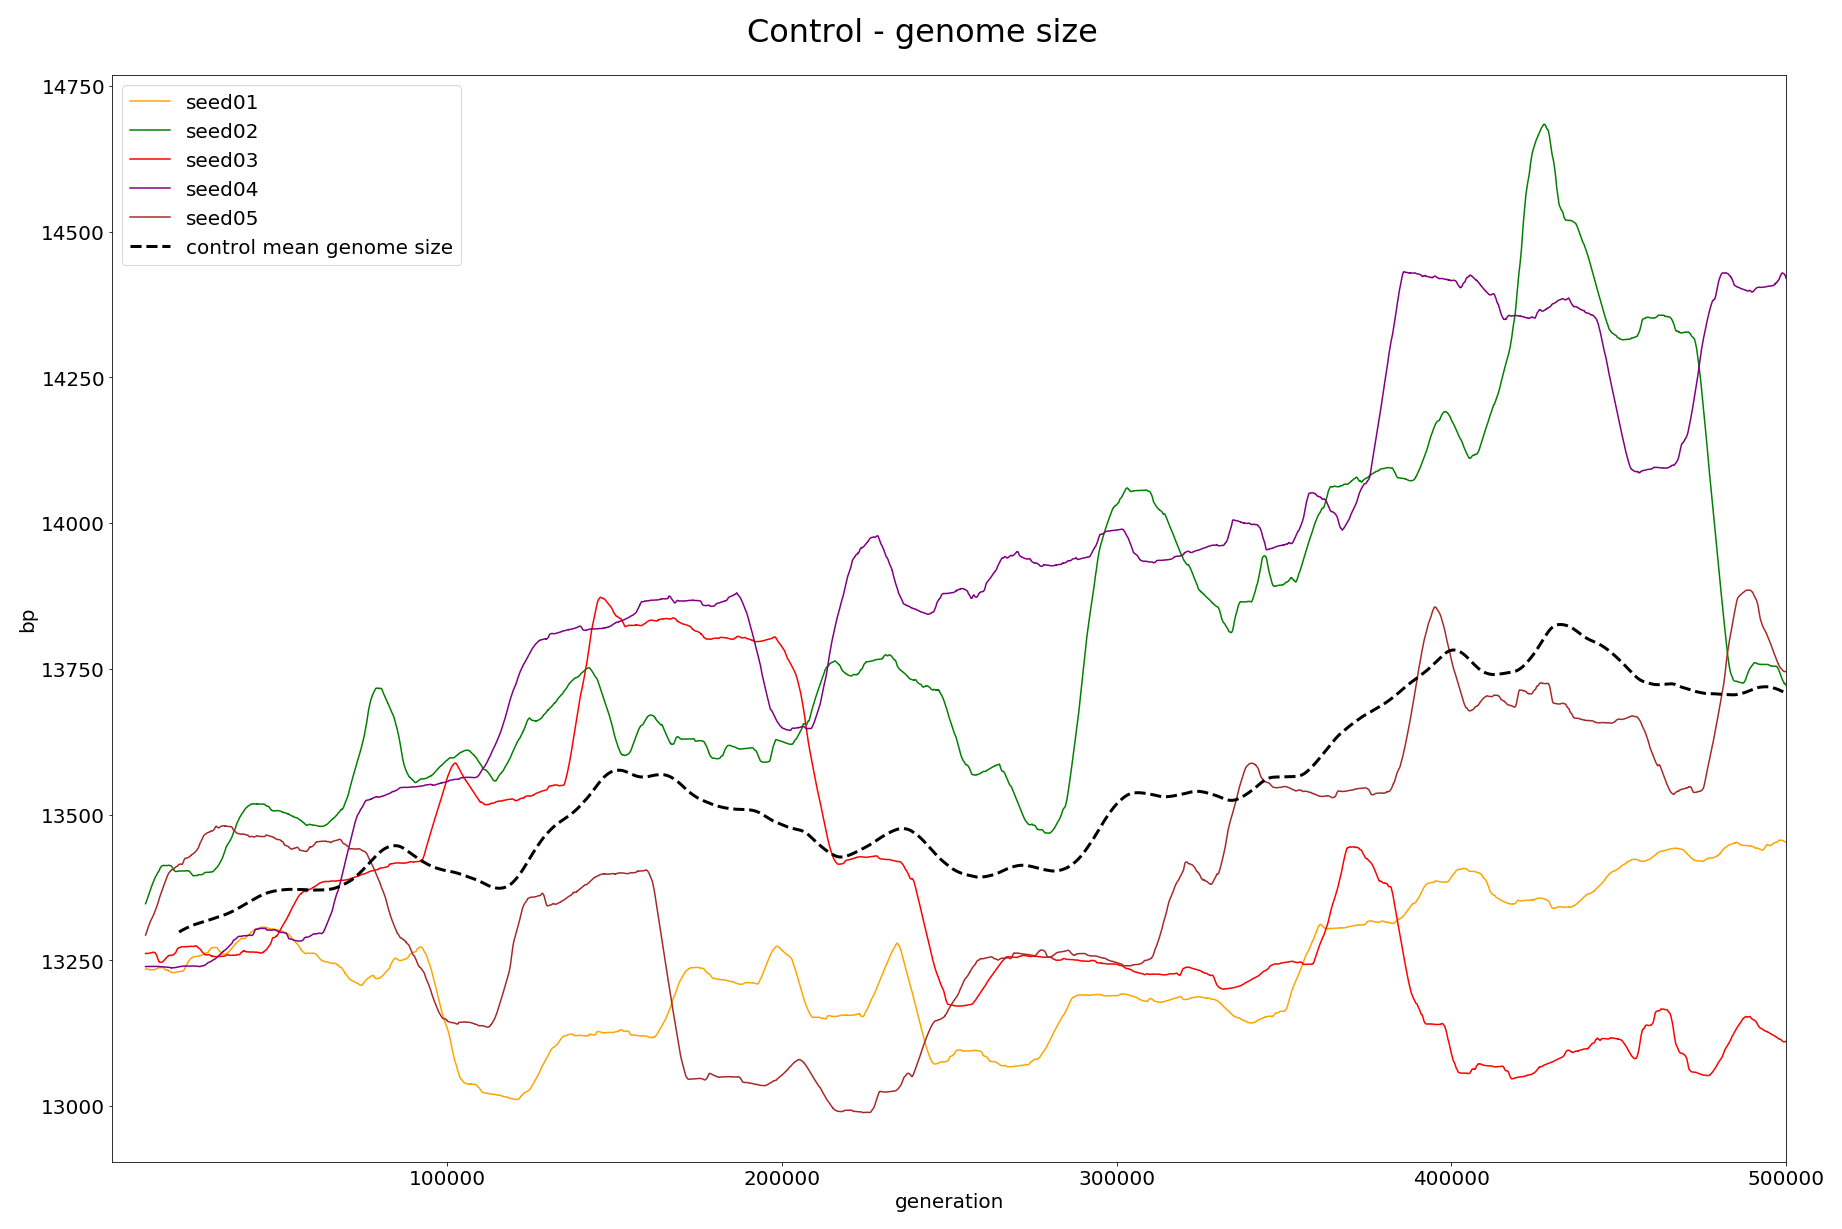
\includegraphics[width=\linewidth]{control_genome_size_b1-e500000}
	\caption[Control genome size, all seeds]{Genome size of the control condition, generations 1-500,000. The individual seeds are shown in various colors and the mean across all seeds is shown in the dashed black line.}
	\label{fig:control_genome_size}
\end{figure}

Examining the figure, over the course of 500,000 generations the mean genome size in the control condition tended towards \textit{gaining} base pairs, averaging just under approximately 500 new base pairs across all seeds. As can be seen in Figure~\ref{fig:control_perc_non-coding}, the averaging out to a modest gain in overall genome size was partially the result of the accumulation of non-coding bases.

% CONTROL PERCENT NON-CODING
\begin{figure}[h]
	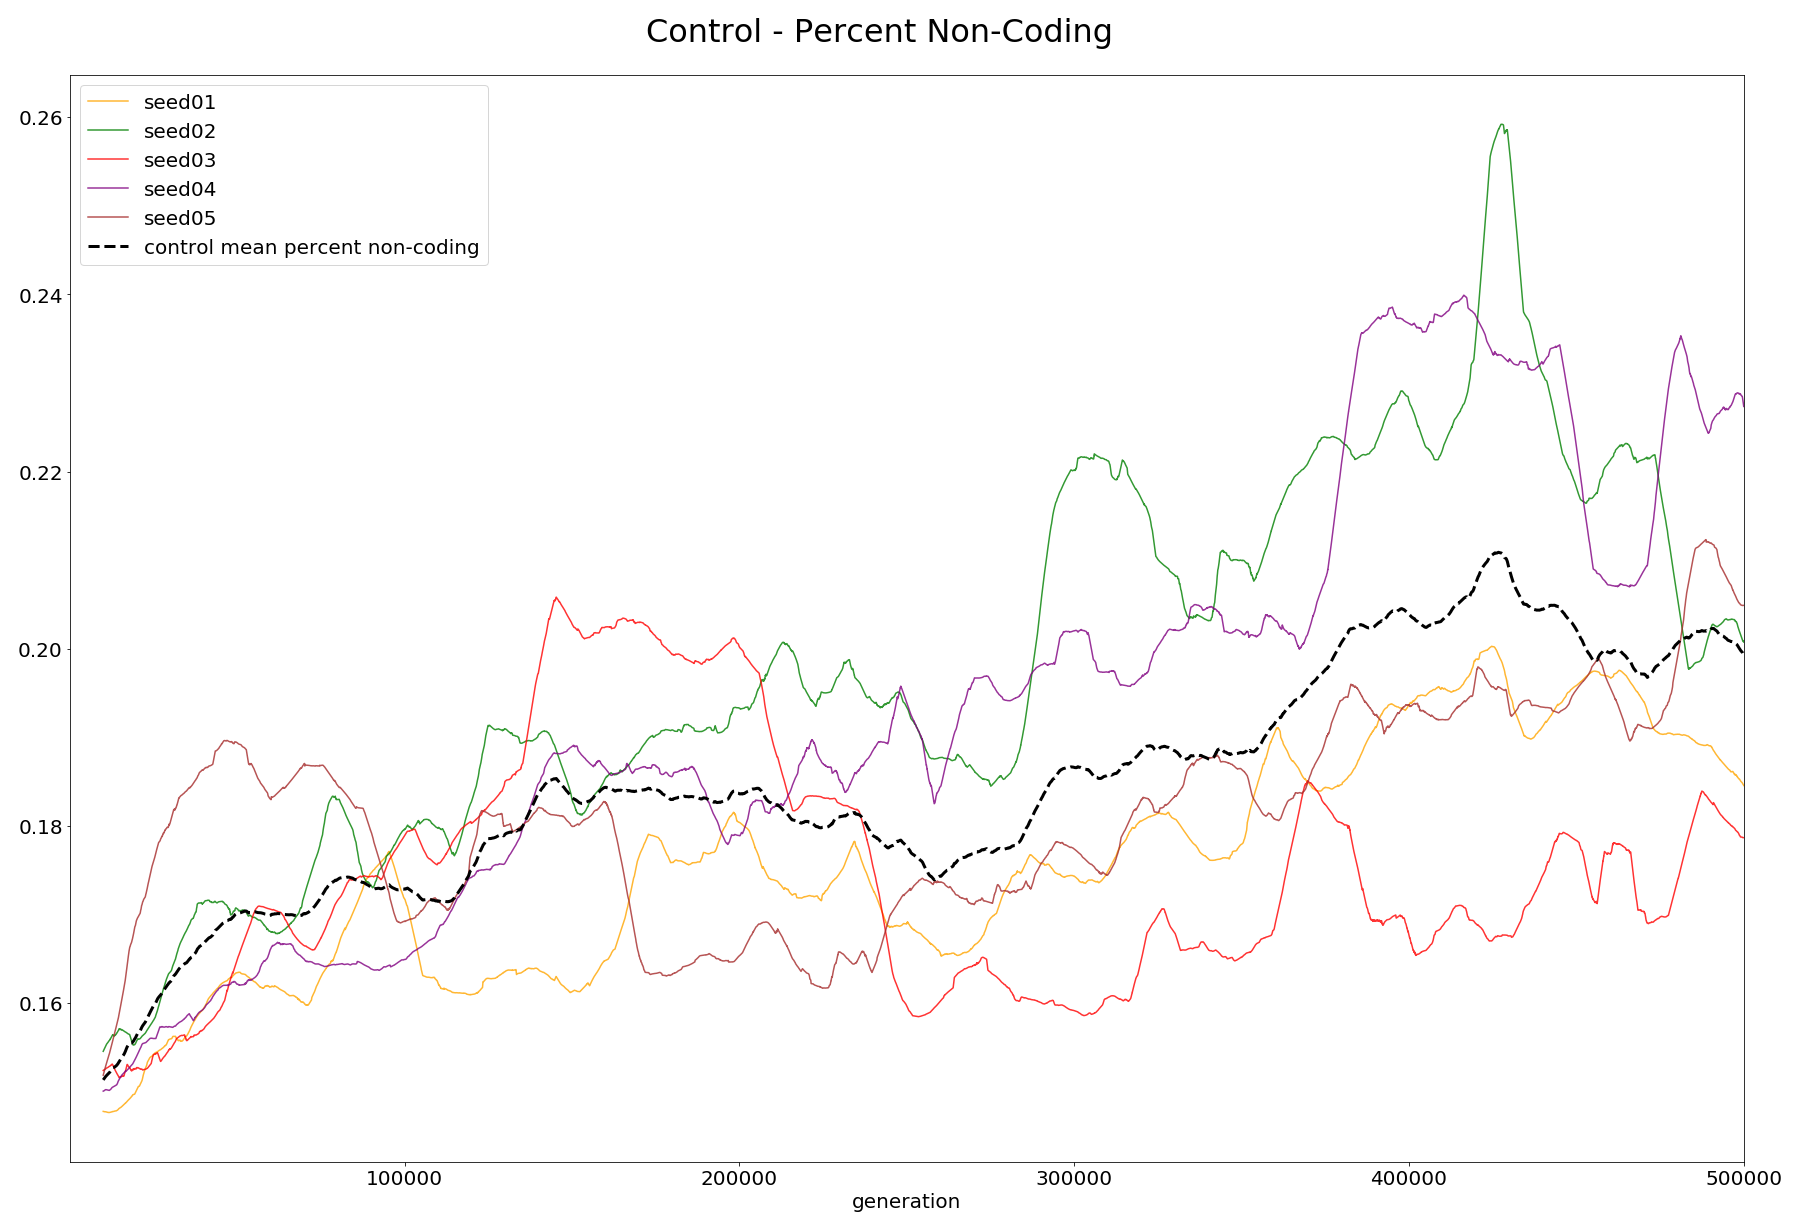
\includegraphics[width=\linewidth]{control_percent_non-coding_b1-e500000}
	\caption[Control condition percent non-coding]{Percent non-coding for the control condition, generation 1-500,000.}
	\label{fig:control_perc_non-coding}
\end{figure}
Despite the slight increase in non-coding bases, however, overall population fitness continued to improve even though the wild types had already evolved for 500,000 generations in the same environment, as seen in Figure~\ref{fig:control_fitness}.

% CONTROL FITNESS
\begin{figure}[h]
	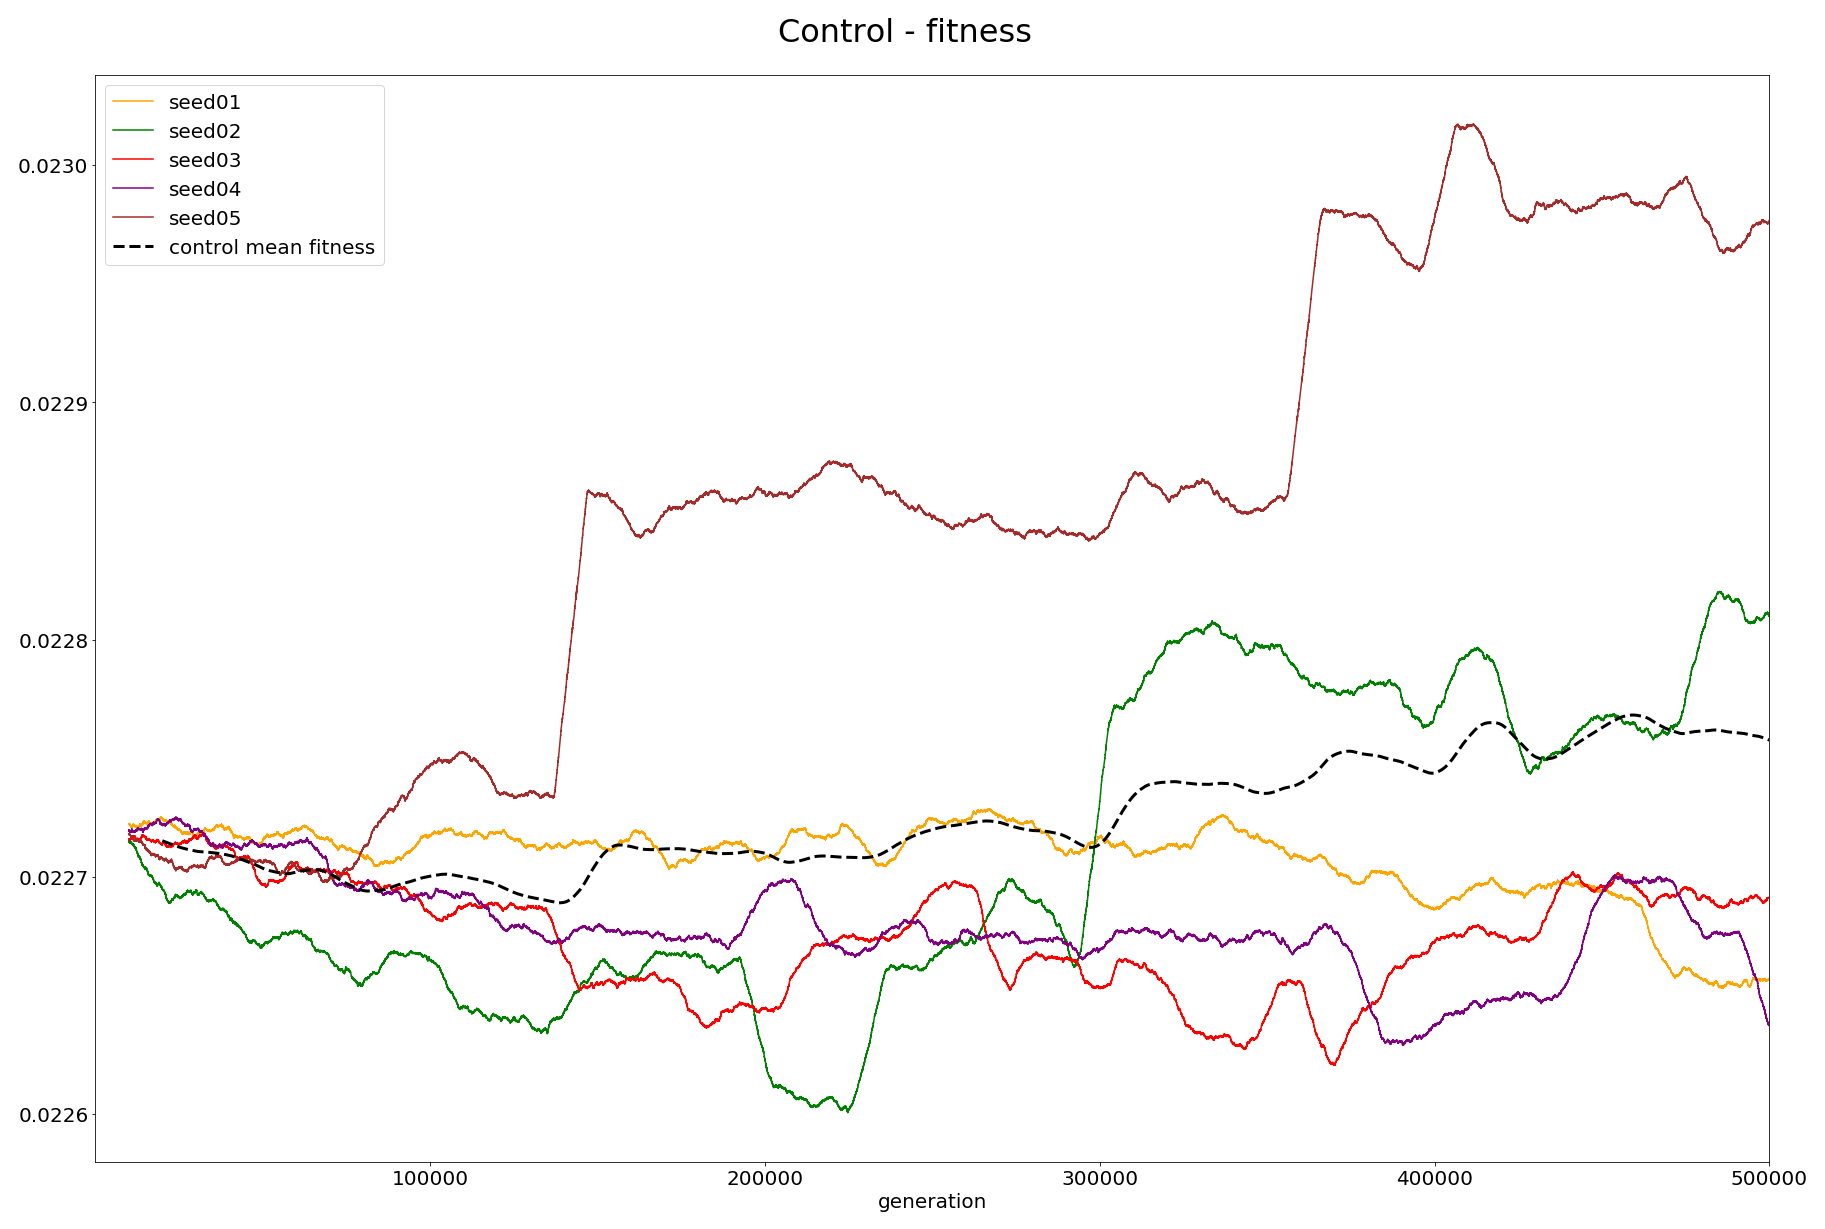
\includegraphics[width=\linewidth]{control_fitness_b1-e500000}
	\caption[Control condition fitness]{Control condition fitness, seeds and mean, generations 1-500,000. The five seeds are in various colors and the mean of these seeds is shown in black, dashed.}
	\label{fig:control_fitness}
\end{figure}

Table~\ref{table:control_mean_fitness_change} below illustrates, however, that although the largest individual fitness improvement in a seed (seed05) was closer to 1.322\%, the improvement in the all-seed mean from the first 50,000 generations to the last 50,000 generations was only 0.2333\%, a very modest increase. 

\begin{table}[H]
	\centering
	\begin{tabular}{|c|c|c|}
		\hline
		\multicolumn{3}{|c|}{\Large \textbf{Control Mean Fitness, All Seeds}} \\
		\hline
		\textbf{fitness @0-50k} & \textbf{fitness @450k-500k} & \textbf{Percent Change} \\
		\hline \hline
		0.022709775696292796 & 0.02276276339318254 & 0.2333\%  \\
		\hline
		
	\end{tabular}
	\caption[Control Population Mean Fitness, Gens 0-50k, 450k-500k]{Table showing the mean population fitness change from generations 0-50k and 450-500k for all seeds.}
	\label{table:control_mean_fitness_change}
\end{table}

Figure~\ref{fig:control_avg_size_of_functional_genes_b1-e500000} shows the change in the average size of functional genes observed in the control condition for all seeds for all 500,000 generations.  

\begin{figure}[h]
	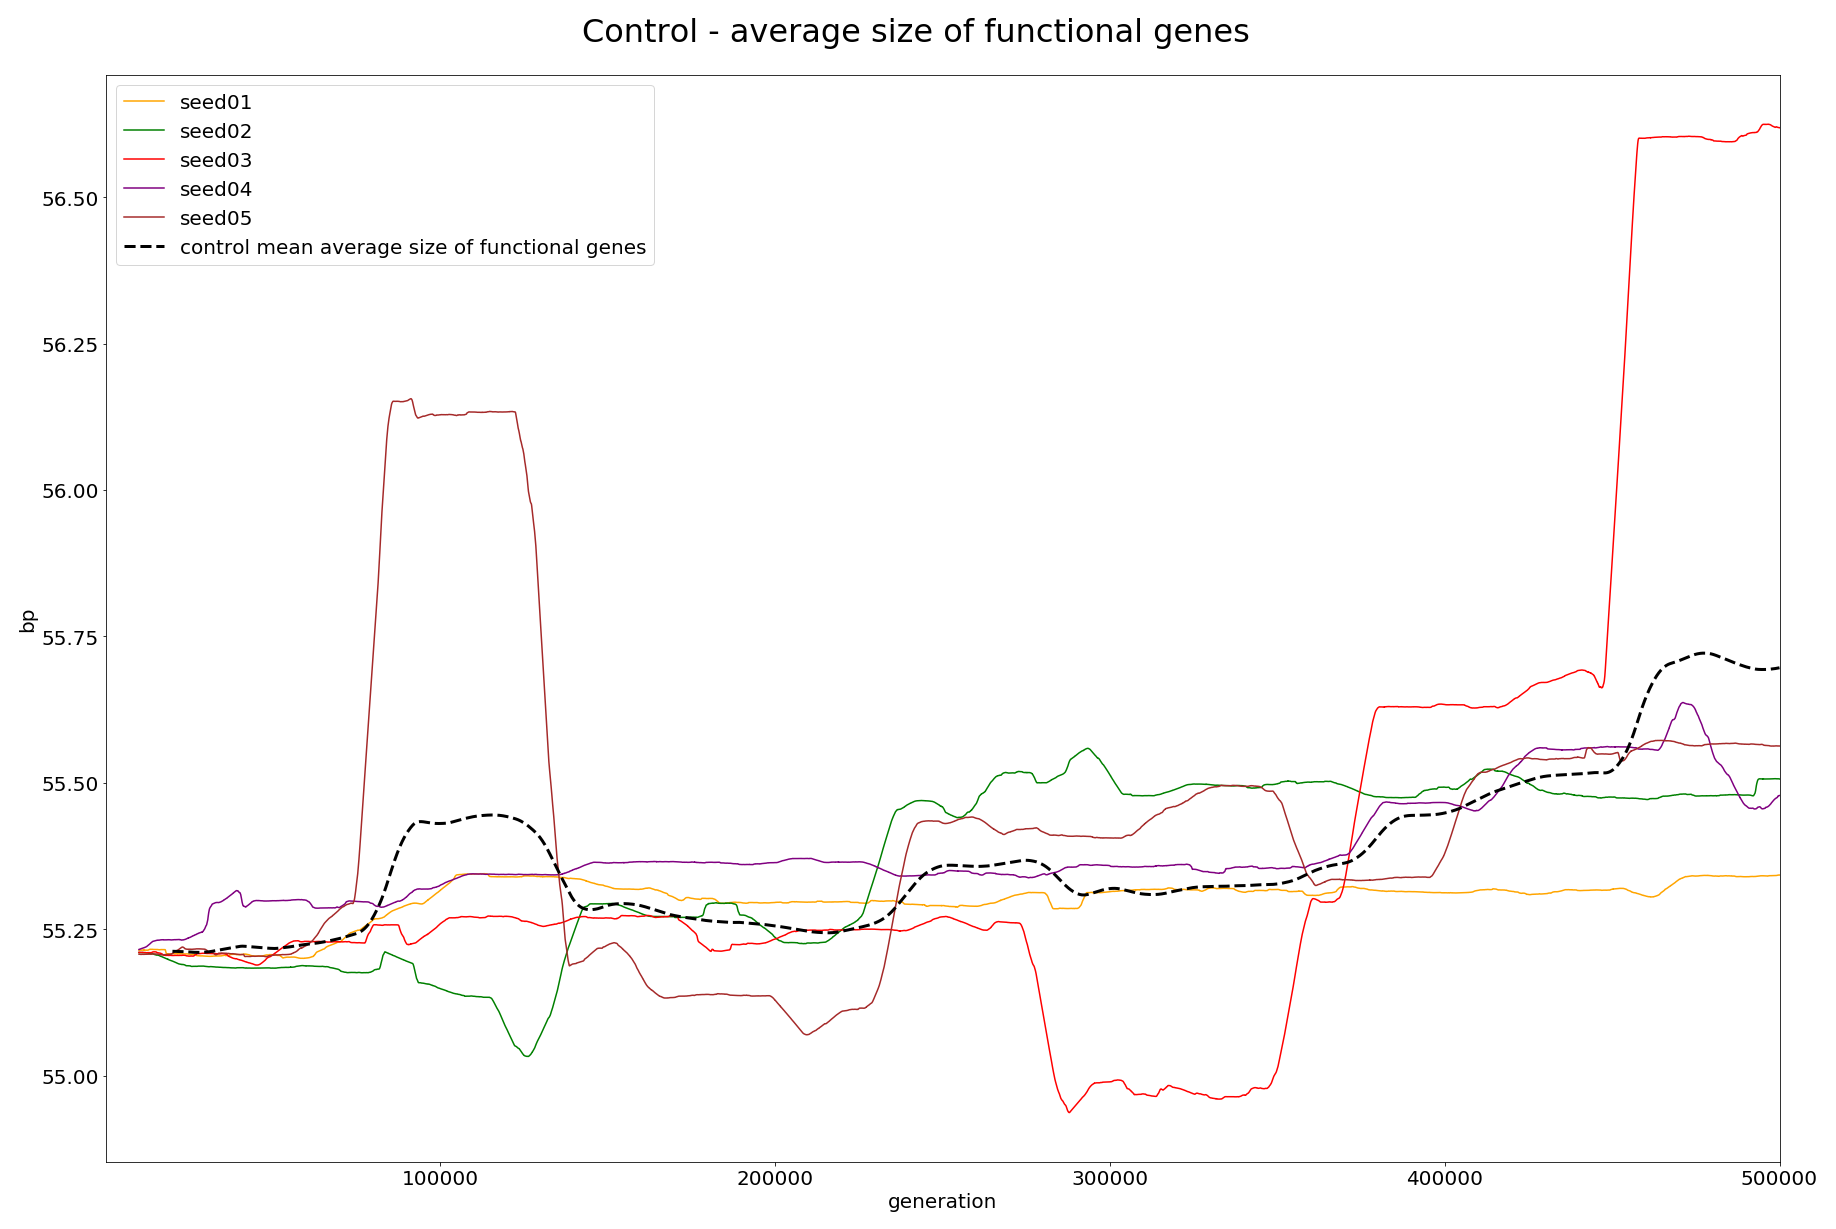
\includegraphics[width=\linewidth]{control_avg_size_of_functional_genes_b1-e500000}
	\caption[Control avg. size of functional genes]{Figure showing the population mean size of the functional genes in the control condition, generations 1-500,000.}
	\label{fig:control_avg_size_of_functional_genes_b1-e500000}
\end{figure}

Figure~\ref{fig:control_gene_density} shows gene density (the number of genes per total number of base pairs). Though this is usually given per million base pairs (Mb), here it is simply the straight number of genes divided by the genome size, and is given as a convenient measure for comparison which takes into account both the number of genes and the genome size. 

\begin{figure}[h]
	\centering
	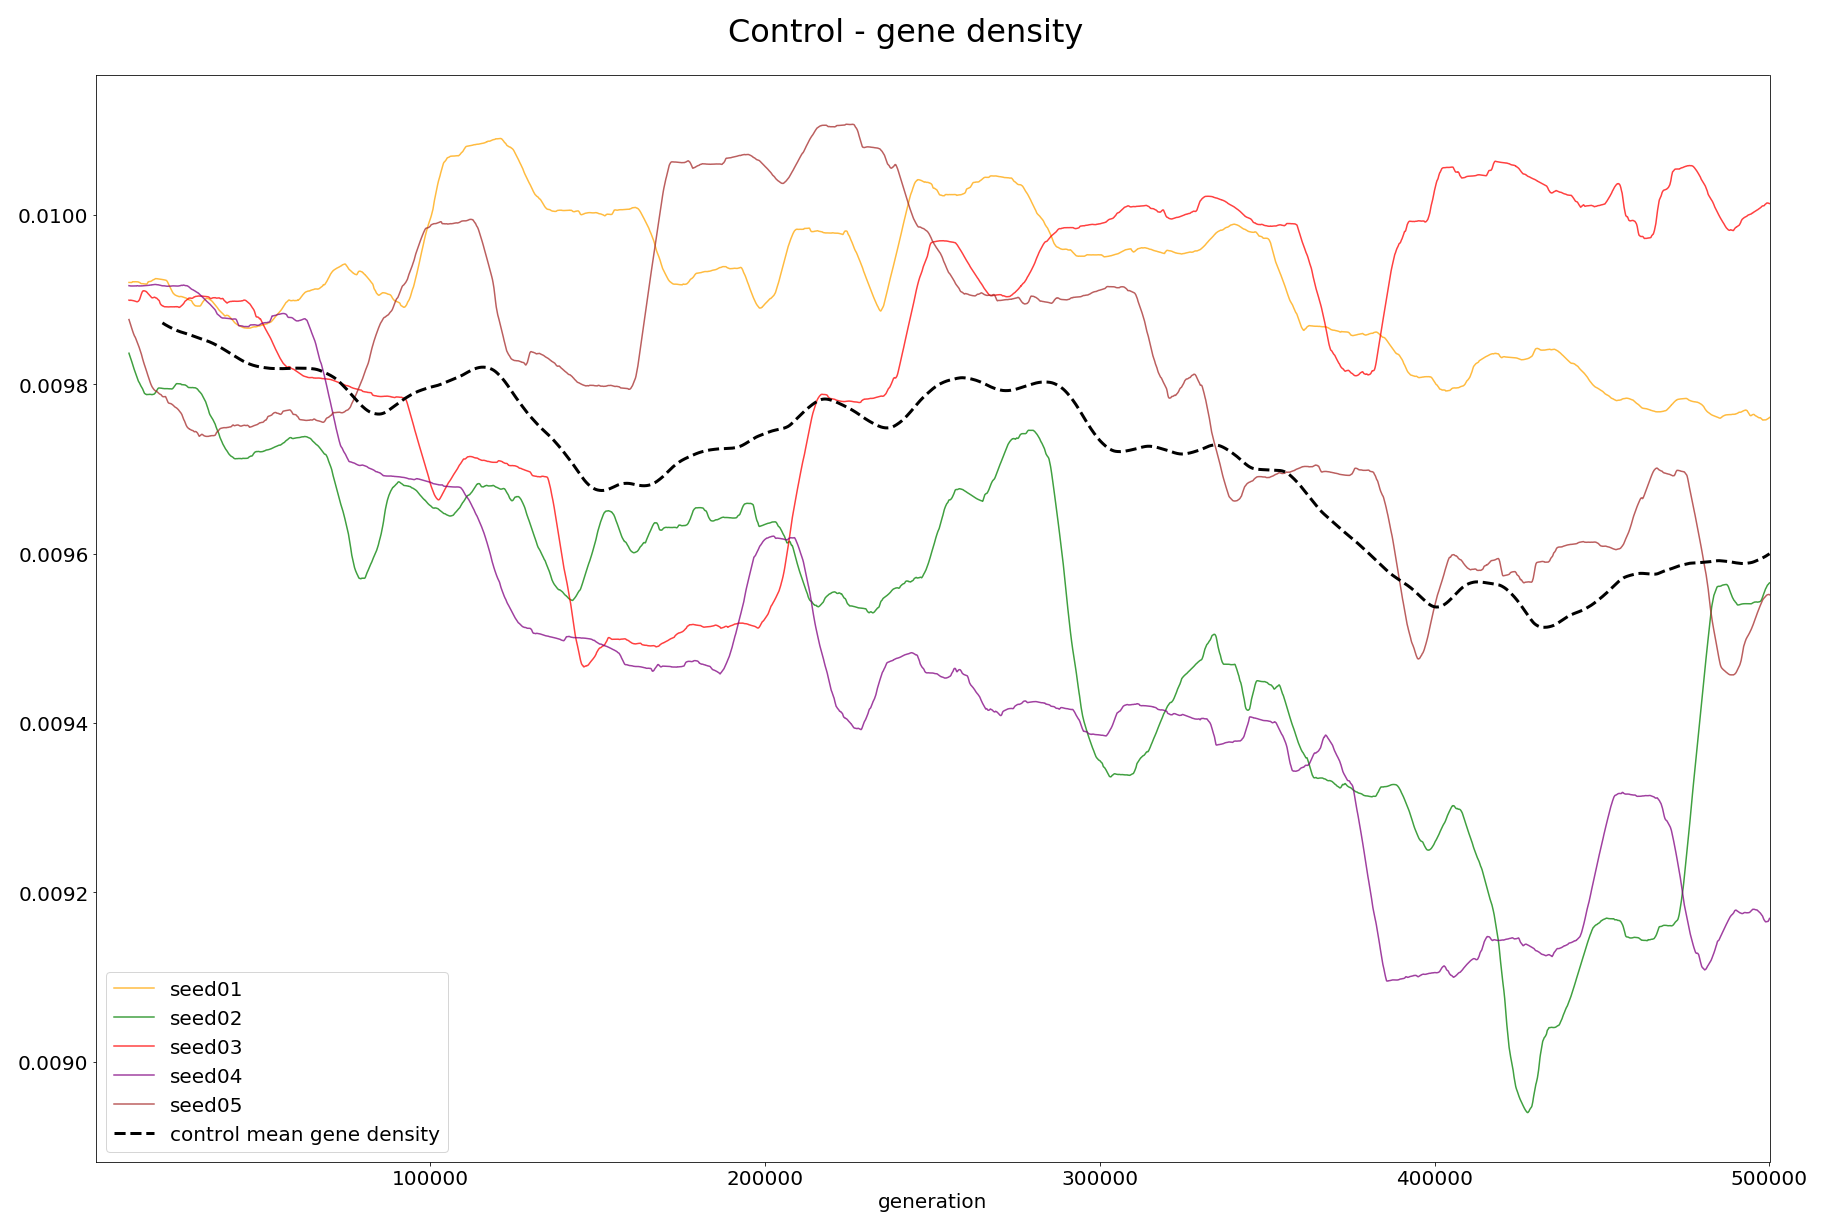
\includegraphics[width=\linewidth]{control_density_b1-e500000}
	\caption[Control gene density]{Control condition gene density, generations 1 to 500,000, all seeds}
	\label{fig:control_gene_density}
\end{figure}

Figures~\ref{fig:control_robustness} and Figure~\ref{fig:control_evolvability} show the control condition's robustness and evolvability, respectively. As a reminder, in Aevol, mutational robustness is calculated by finding the fraction of neutral offspring of an individual. In these figures, both robustness and evolvability are calculated based on the best individual at generation 500,000. Please note the scale of Figure~\ref{fig:control_evolvability}, which is $1*e^{-8}$.

\begin{figure}[h]
	\centering
	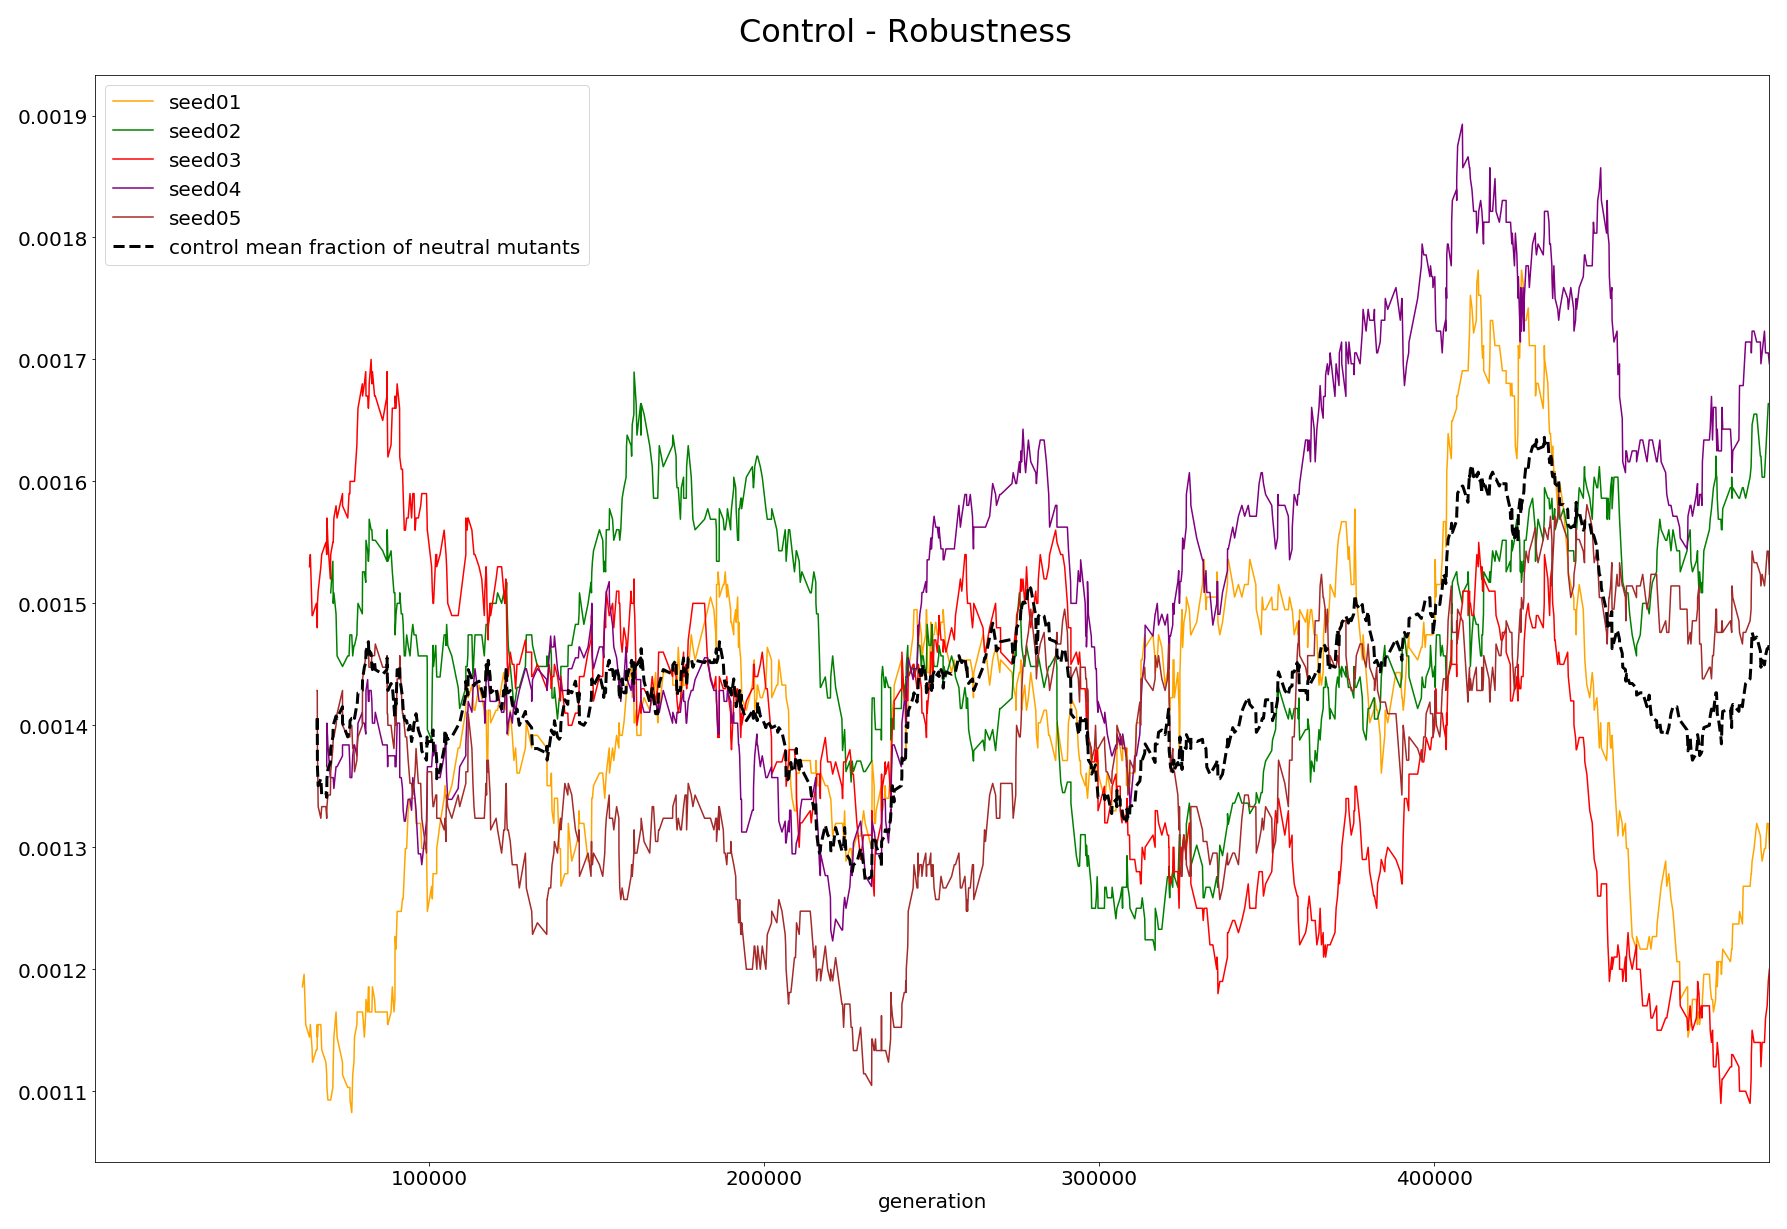
\includegraphics[width=\linewidth]{control_frac_neutral_mutants_b1-e500000}
	\caption[Control robustness]{Control robustness for generations 1-500,000, all seeds.}
	\label{fig:control_robustness}
\end{figure}

\begin{figure}[h]
	\centering
	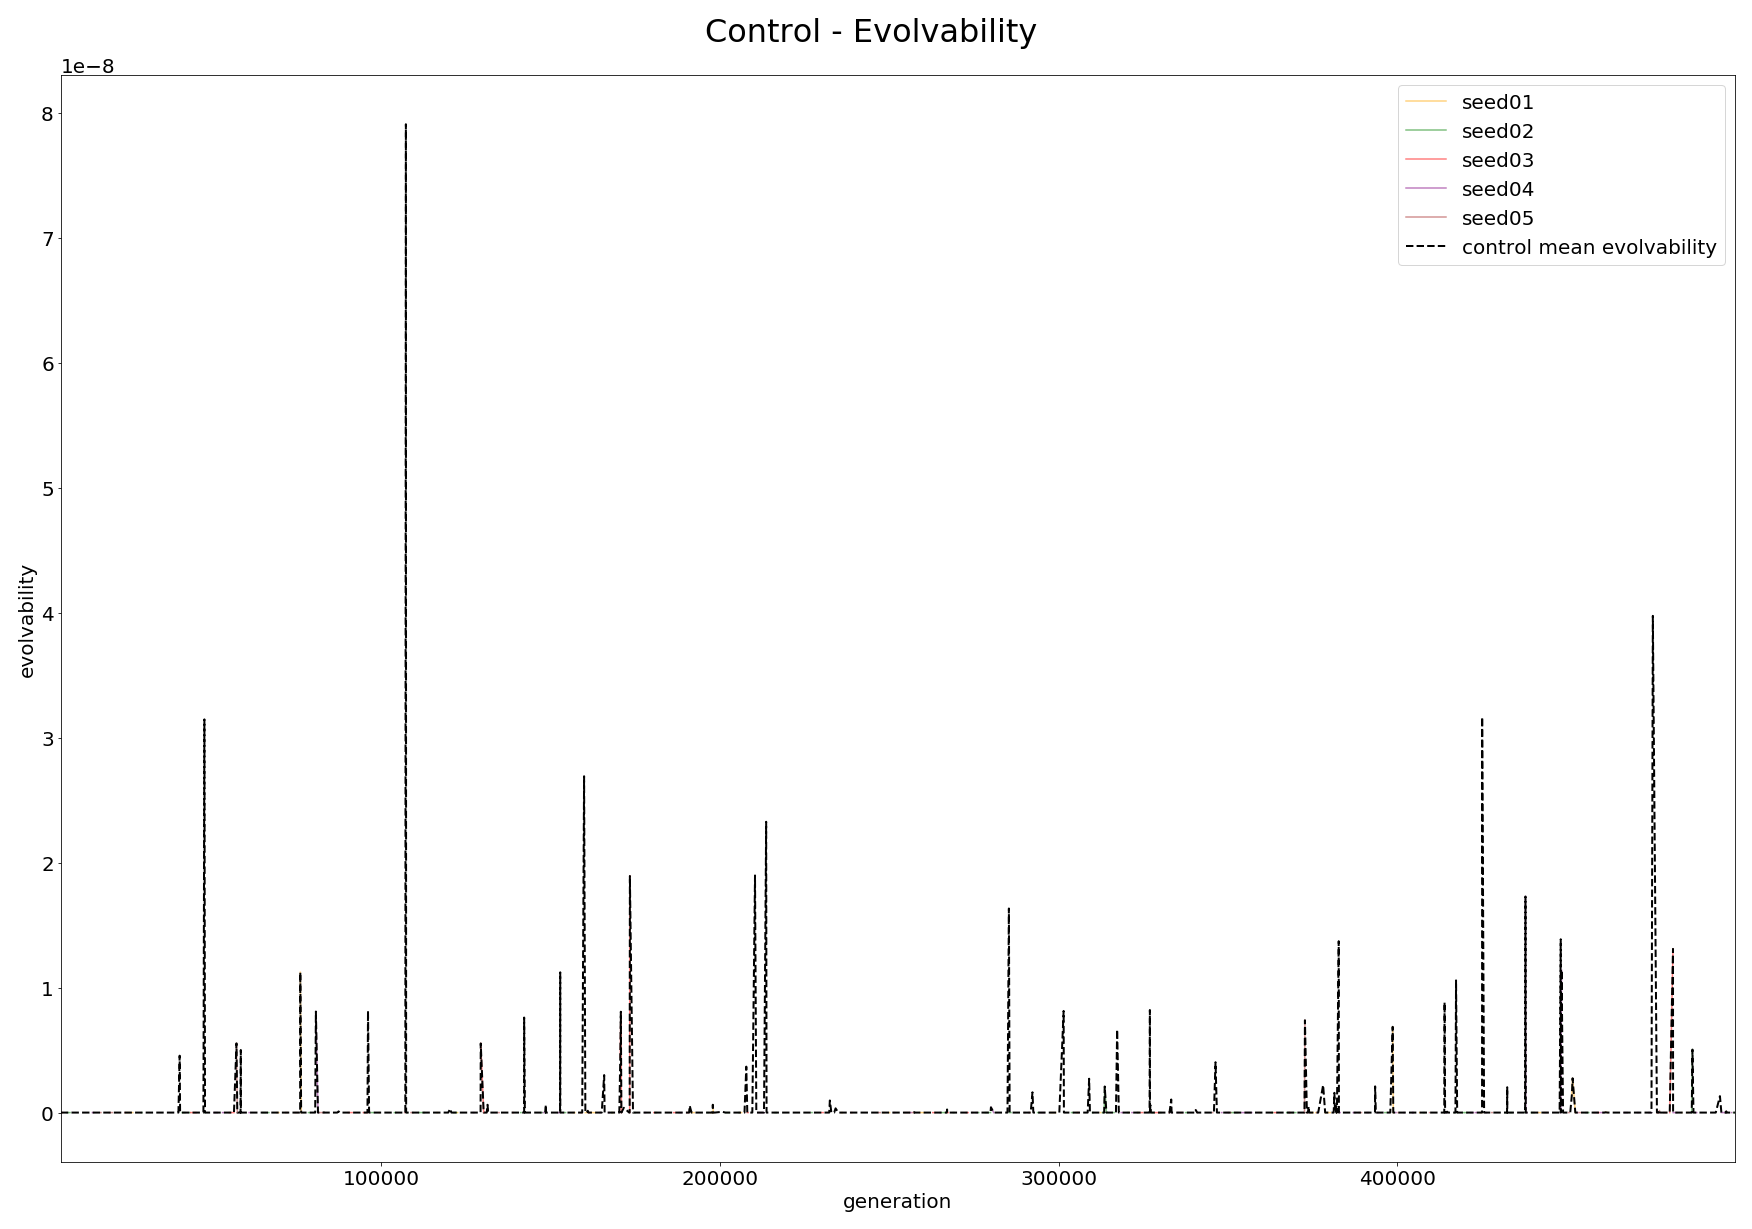
\includegraphics[width=\linewidth]{control_evolvability_b1-e500000}
	\caption[Control evolvability]{Control evolvability, all seeds.}
	\label{fig:control_evolvability}
\end{figure}
Because the wild types began these experiments having evolved for 10 million generations in a static environment, their variability was low and the genome was relatively compact (thanks to the natural streamlining effects of bacterial genomes), and thus their mutational robustness was also low.
% MUTATION UP
\subsection{Mutation Up}
The genome size for the $\mu_+$ condition is shown in Figure~\ref{fig:mut_up_genome_size}. The $\mu_+$ population mean genome size fluctuated between being above and below the control condition, and Table~\ref{table:genome_size_mean_and_std_dev} (pg. \pageref{table:genome_size_mean_and_std_dev}) makes it clear that, when considered over the whole run of 500,000 generations, the increased mutation rate lead to a slightly \textit{larger} mean genome size (0.157661\%). 
\begin{figure}[H]
	\centering
	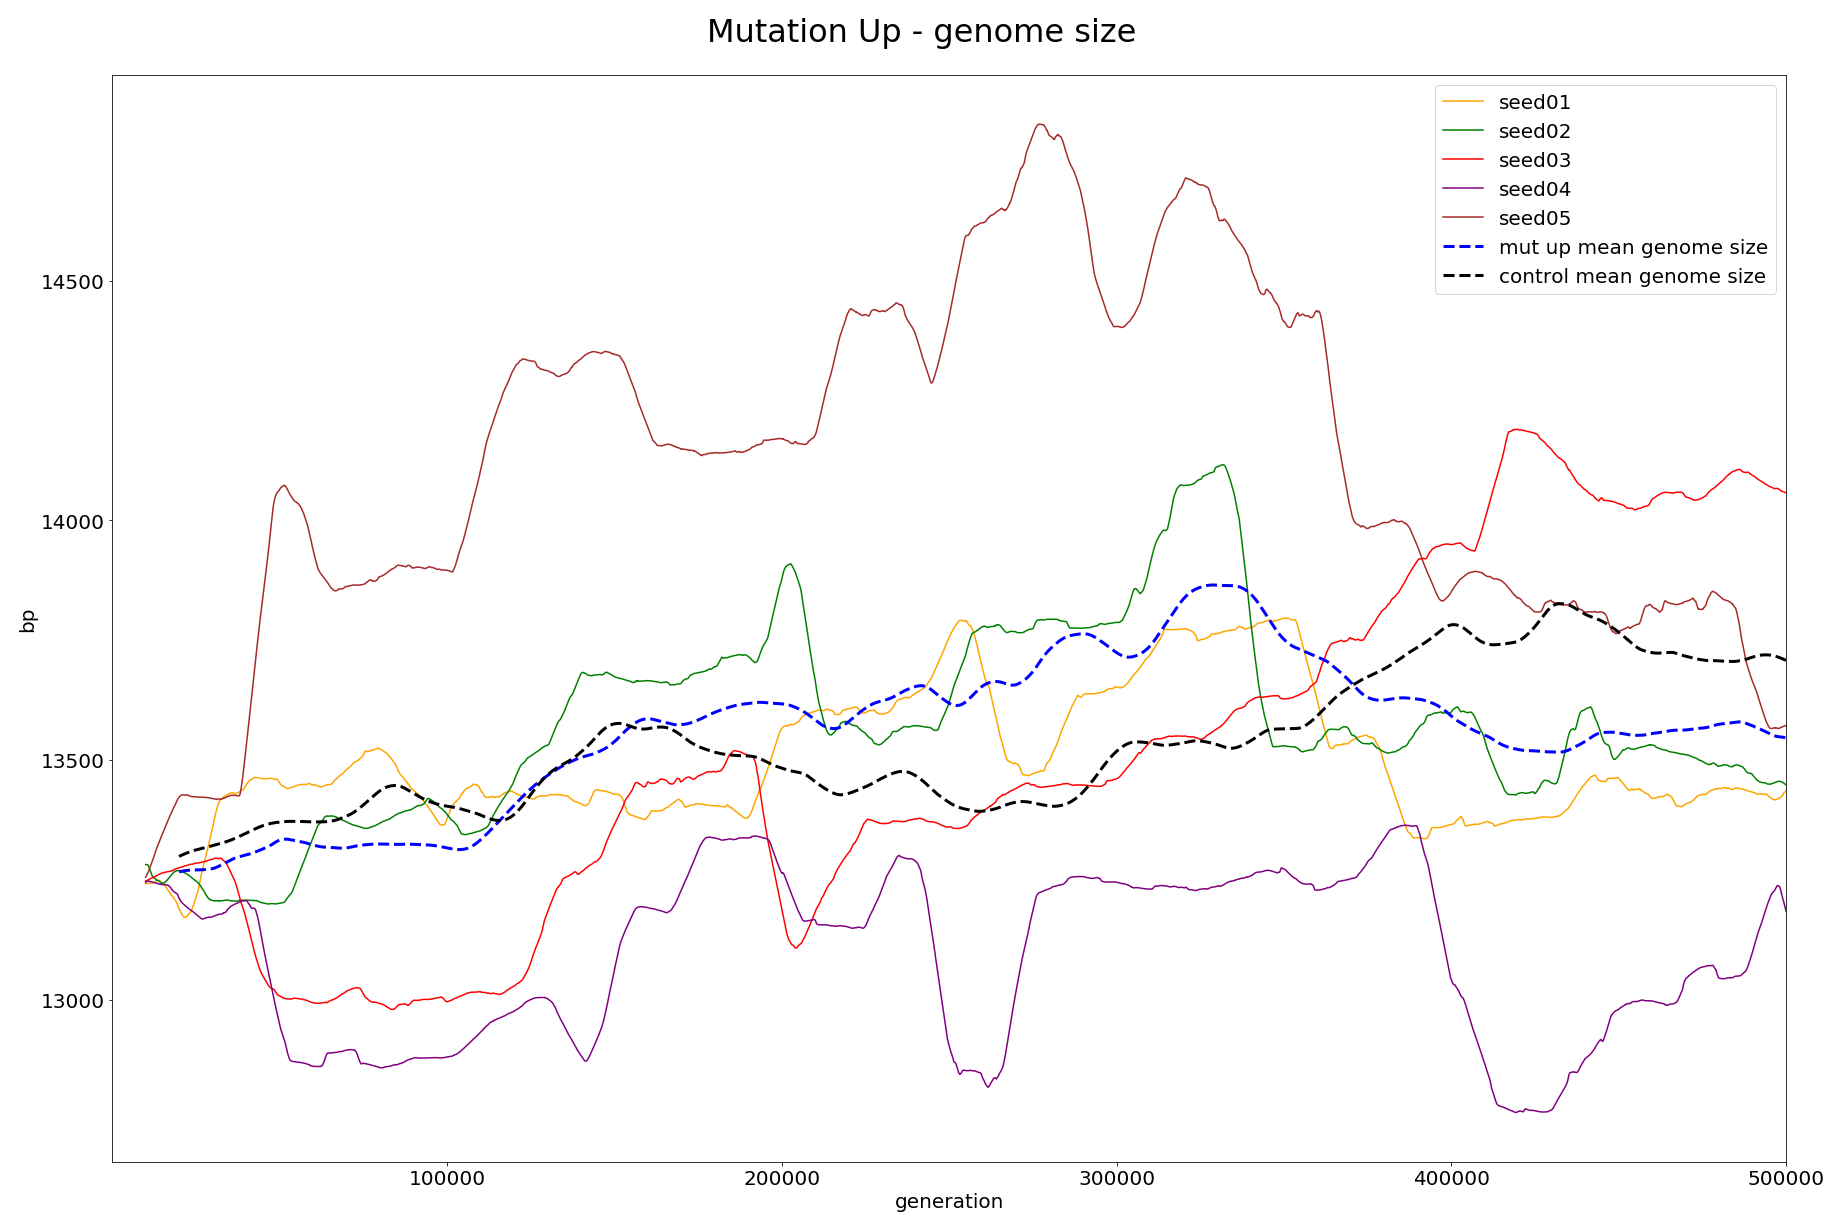
\includegraphics[width=\linewidth]{mut_up_genome_size_b1-e500000}
	\caption[Mutation down genome size]{$\mu_+$ population genome size, generations 1-500,000.}
	\label{fig:mut_up_genome_size}
\end{figure}

At first glance, this increase in genome size over the whole run seems to counter the prediction based on Liard et al.~\cite{Liard.2018} as discussed in Section~\ref{related_work:reductive_evolution}. Based on their research, in the $\mu_+$ condition, an increased mutation rate is expected to boost mutational robustness by disrupting existing genes and introducing many non-coding bases, which in turn allows purifying selection to overcome the proposed complexity ratchet, finally reducing the genome. If one examines the general trends rather than just the final result, it becomes clear that this does seem to be what happened in these experiments, as well, as the final genome size was below the control condition and seemingly still on its way down. 

Figure~\ref{fig:mut_up_robustness} confirms that, as time went on, the robustness greatly increased over the control condition (blue dashed line vs. black dashed line) and Figure~\ref{fig:mut_up_gene_density} indicates that purifying selection was at work, increasing the gene density. Similarly, Figure~\ref{fig:mut_up_percent_non-coding} shows the initial increase in the number of non-coding bases as genes were disrupted. 

\begin{figure}[h]
	\centering
	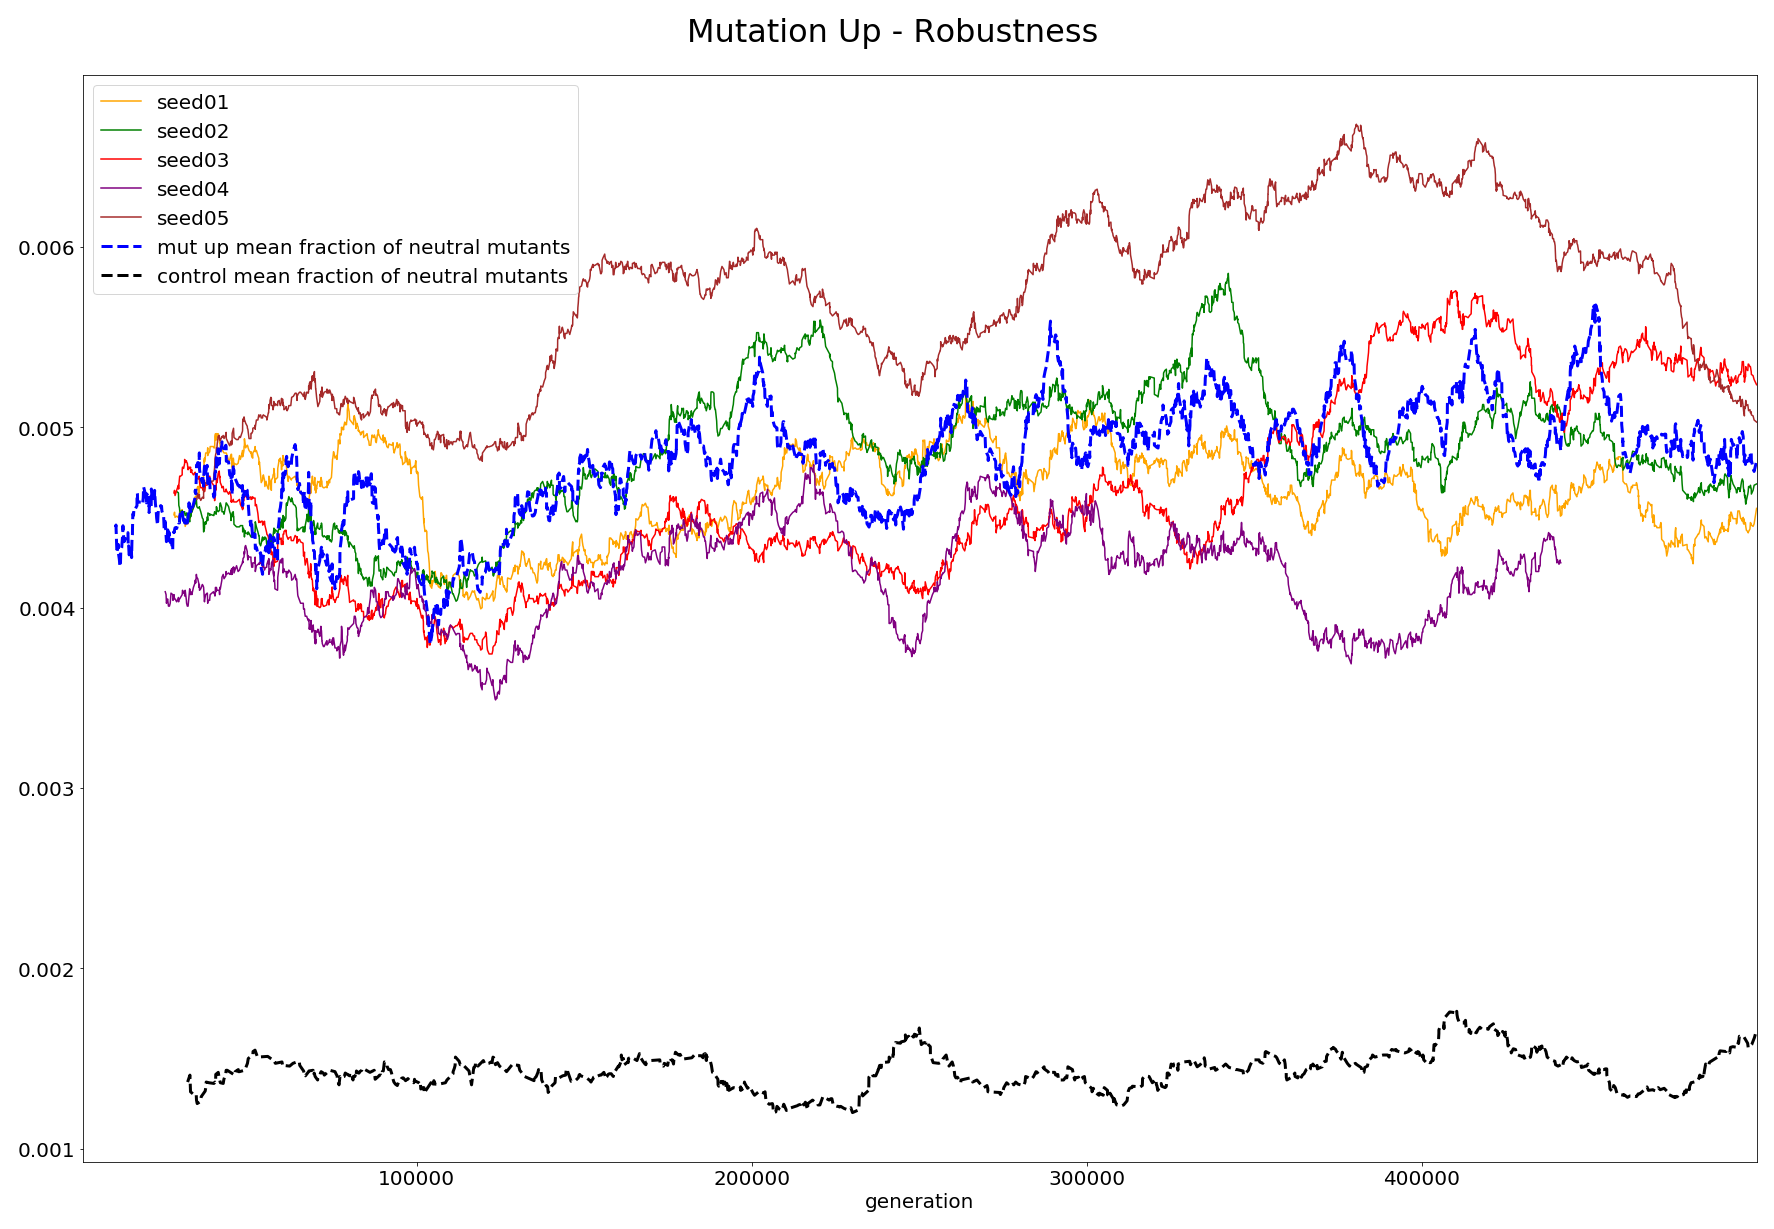
\includegraphics[width=\linewidth]{mut_up_frac_neutral_mutants_b1-e500000}
	\caption[Mutation up robustness]{Mutation up robustness, generations 1-500,000.}
	\label{fig:mut_up_robustness}
\end{figure}

\begin{figure}[h]
	\centering
	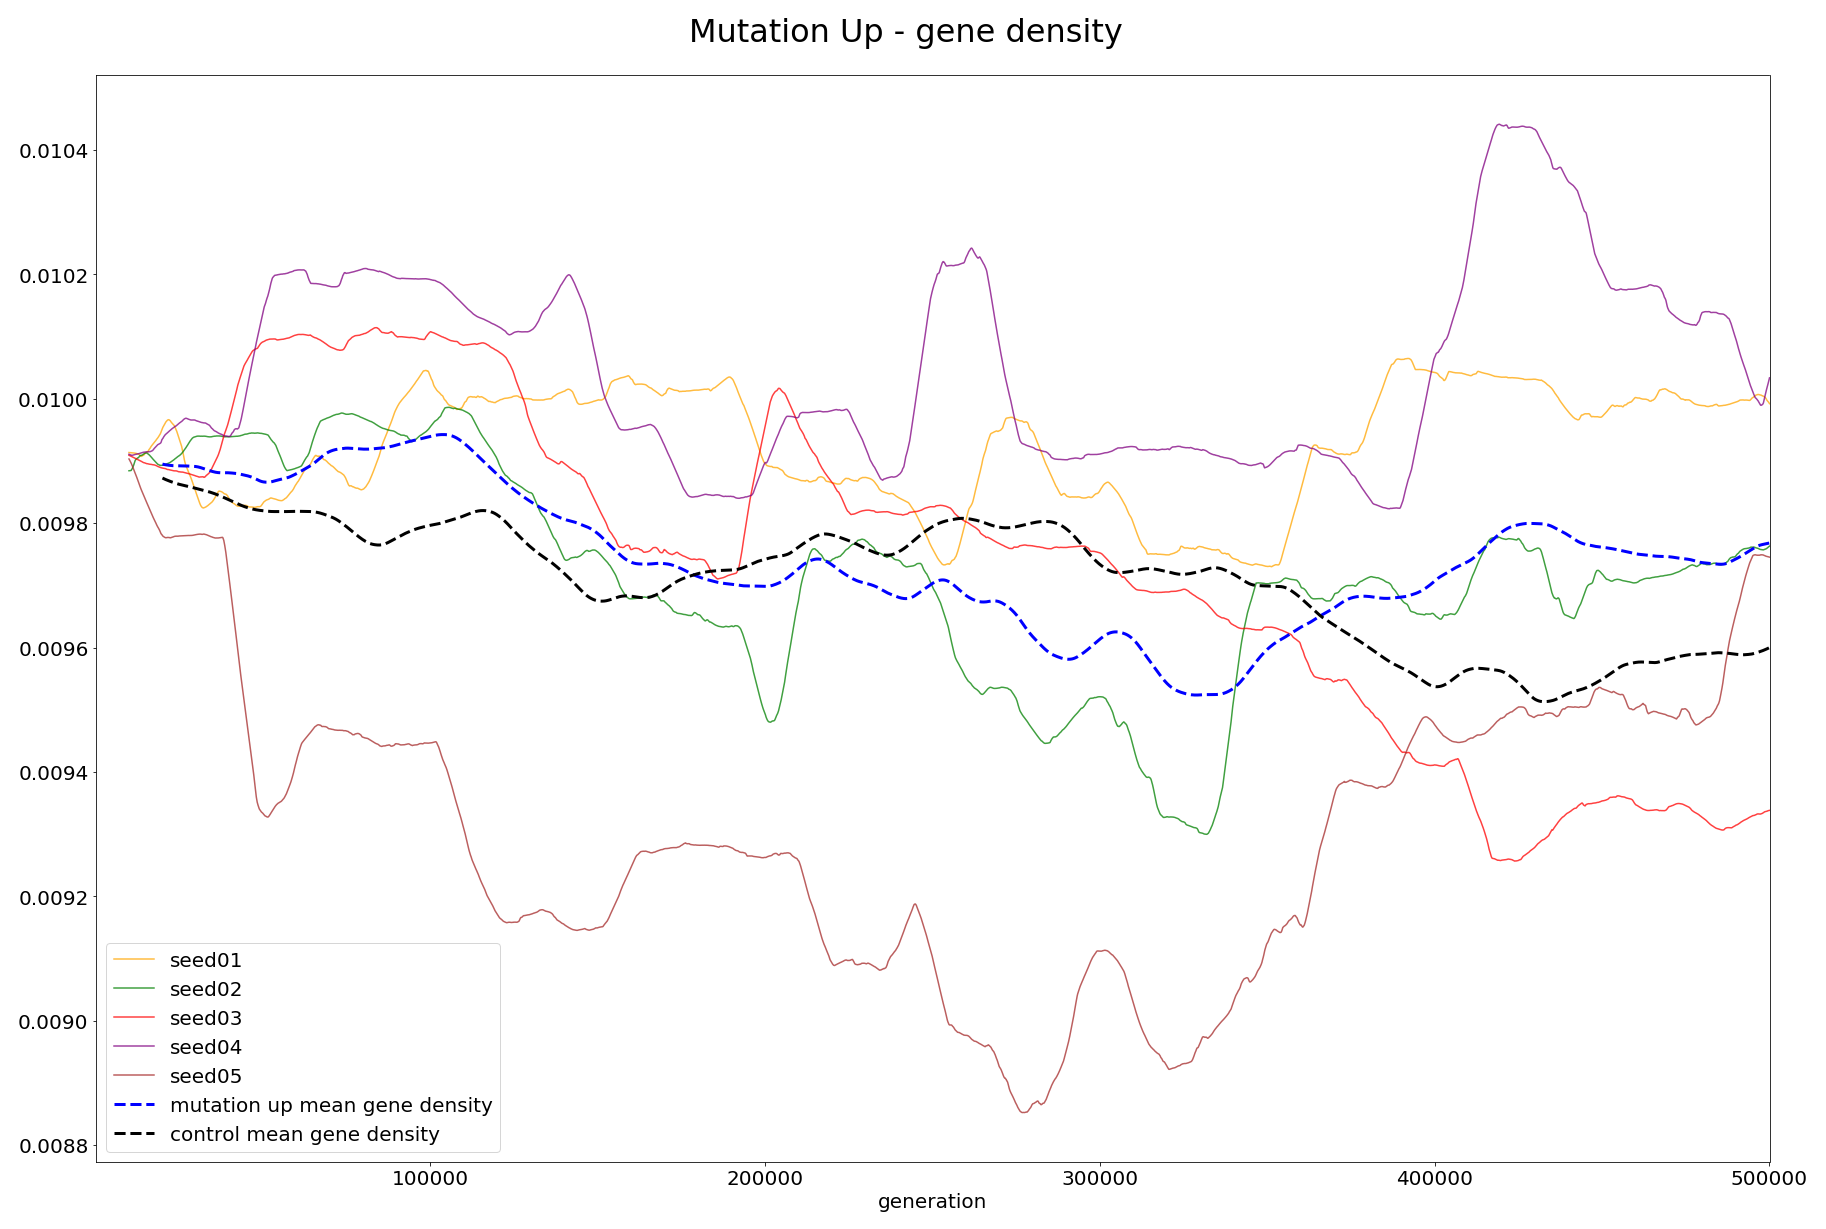
\includegraphics[width=\linewidth]{mut_up_gene_density_b1-e500000}
	\caption[Mutation up gene density]{Mutation up gene density for generations 1-500,000, all seeds.}
	\label{fig:mut_up_gene_density}
\end{figure}

\begin{figure}[h]
	\centering
	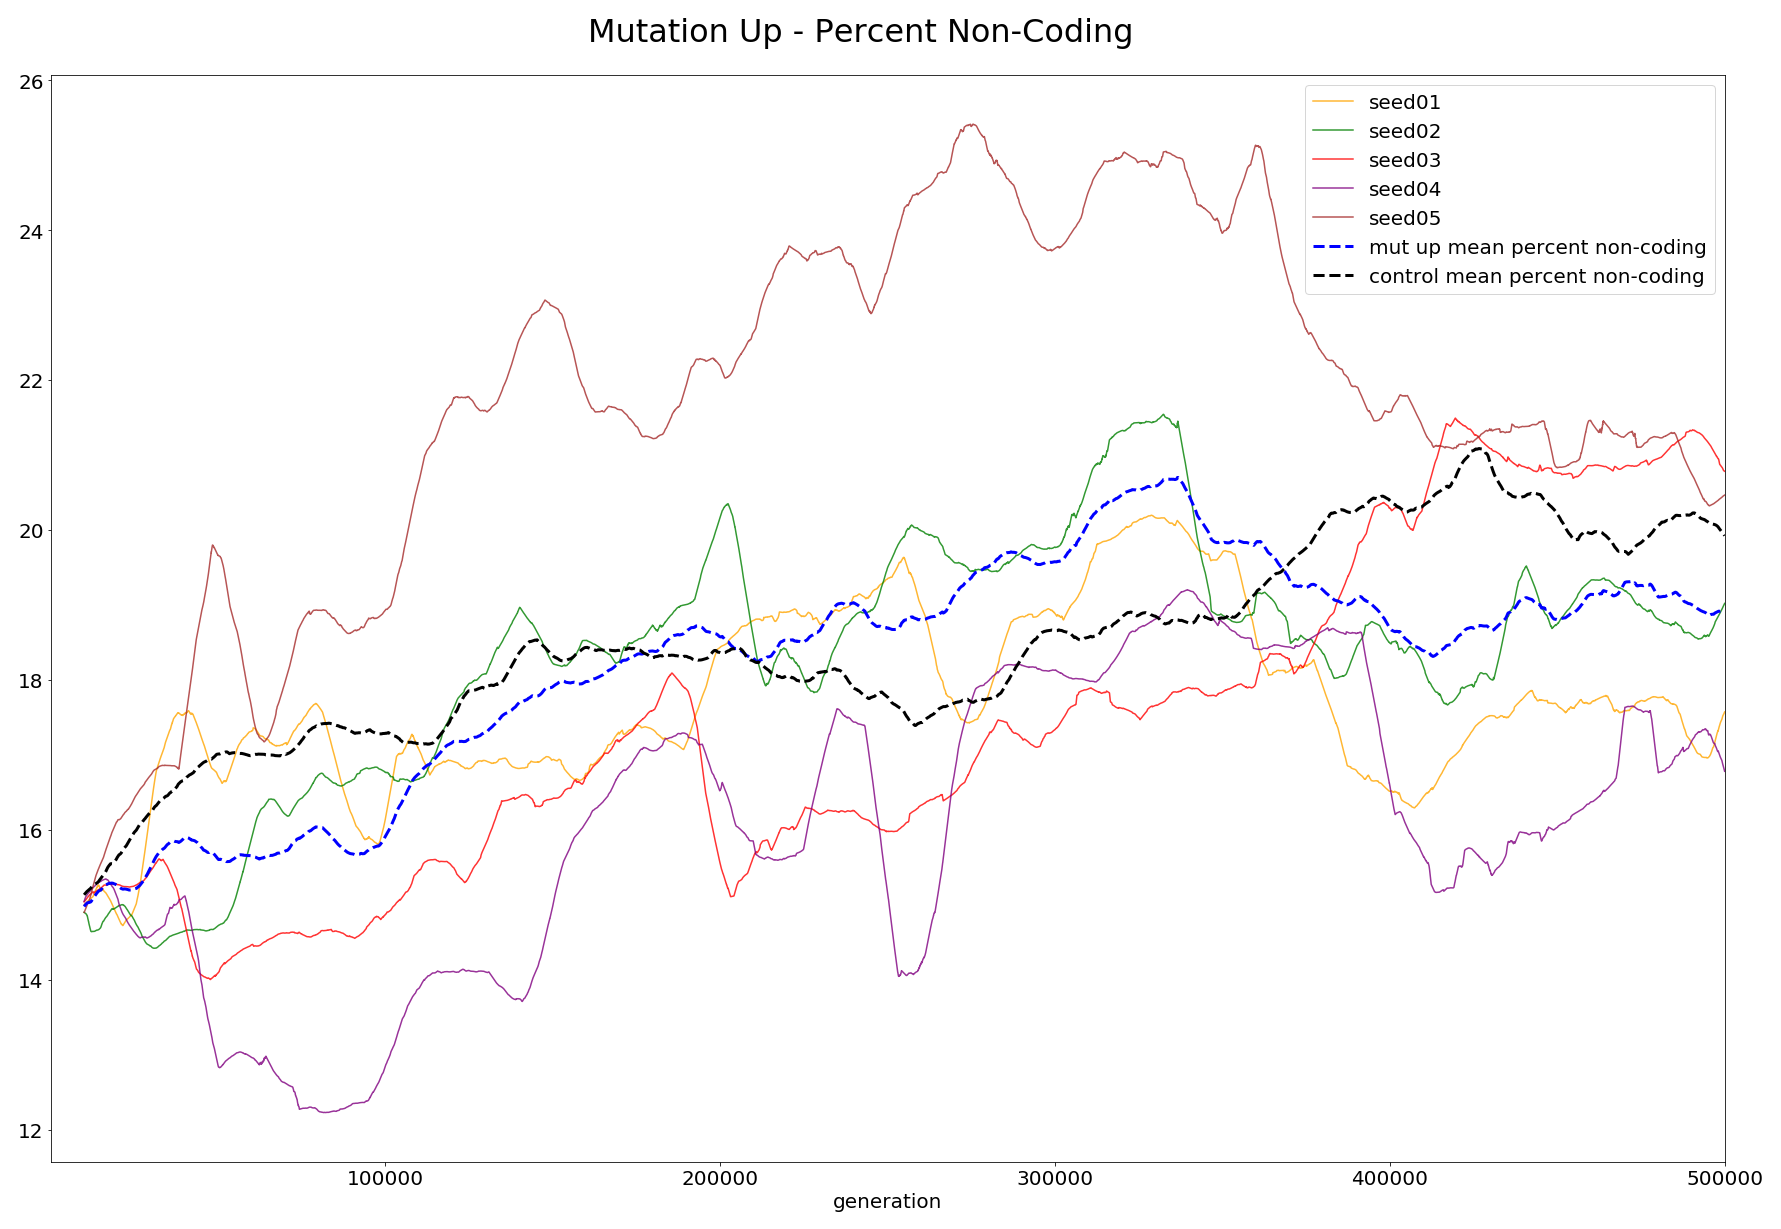
\includegraphics[width=\linewidth]{mut_up_percent_non-coding_b1-e500000}
	\caption[Mutation up - percent non-coding]{$\mu_+$ percent non-coding}
	\label{fig:mut_up_percent_non-coding}
\end{figure}

% MUTATION DOWN
\subsection{Mutation Down}
The results of decreasing the mutation rate to $2.5e-8$ from the usual $1e-7$ also had the unexpected result (according to the predictions from Section~\ref{sec:expected_results}) that the genome size decreased over the control condition, though it still did not end up being lower than at generation 1. Figure~\ref{fig:mut_down:genome_size} shows the data for the genome size of the $\mu_-$ condition.
\begin{figure}[H]
	\centering
	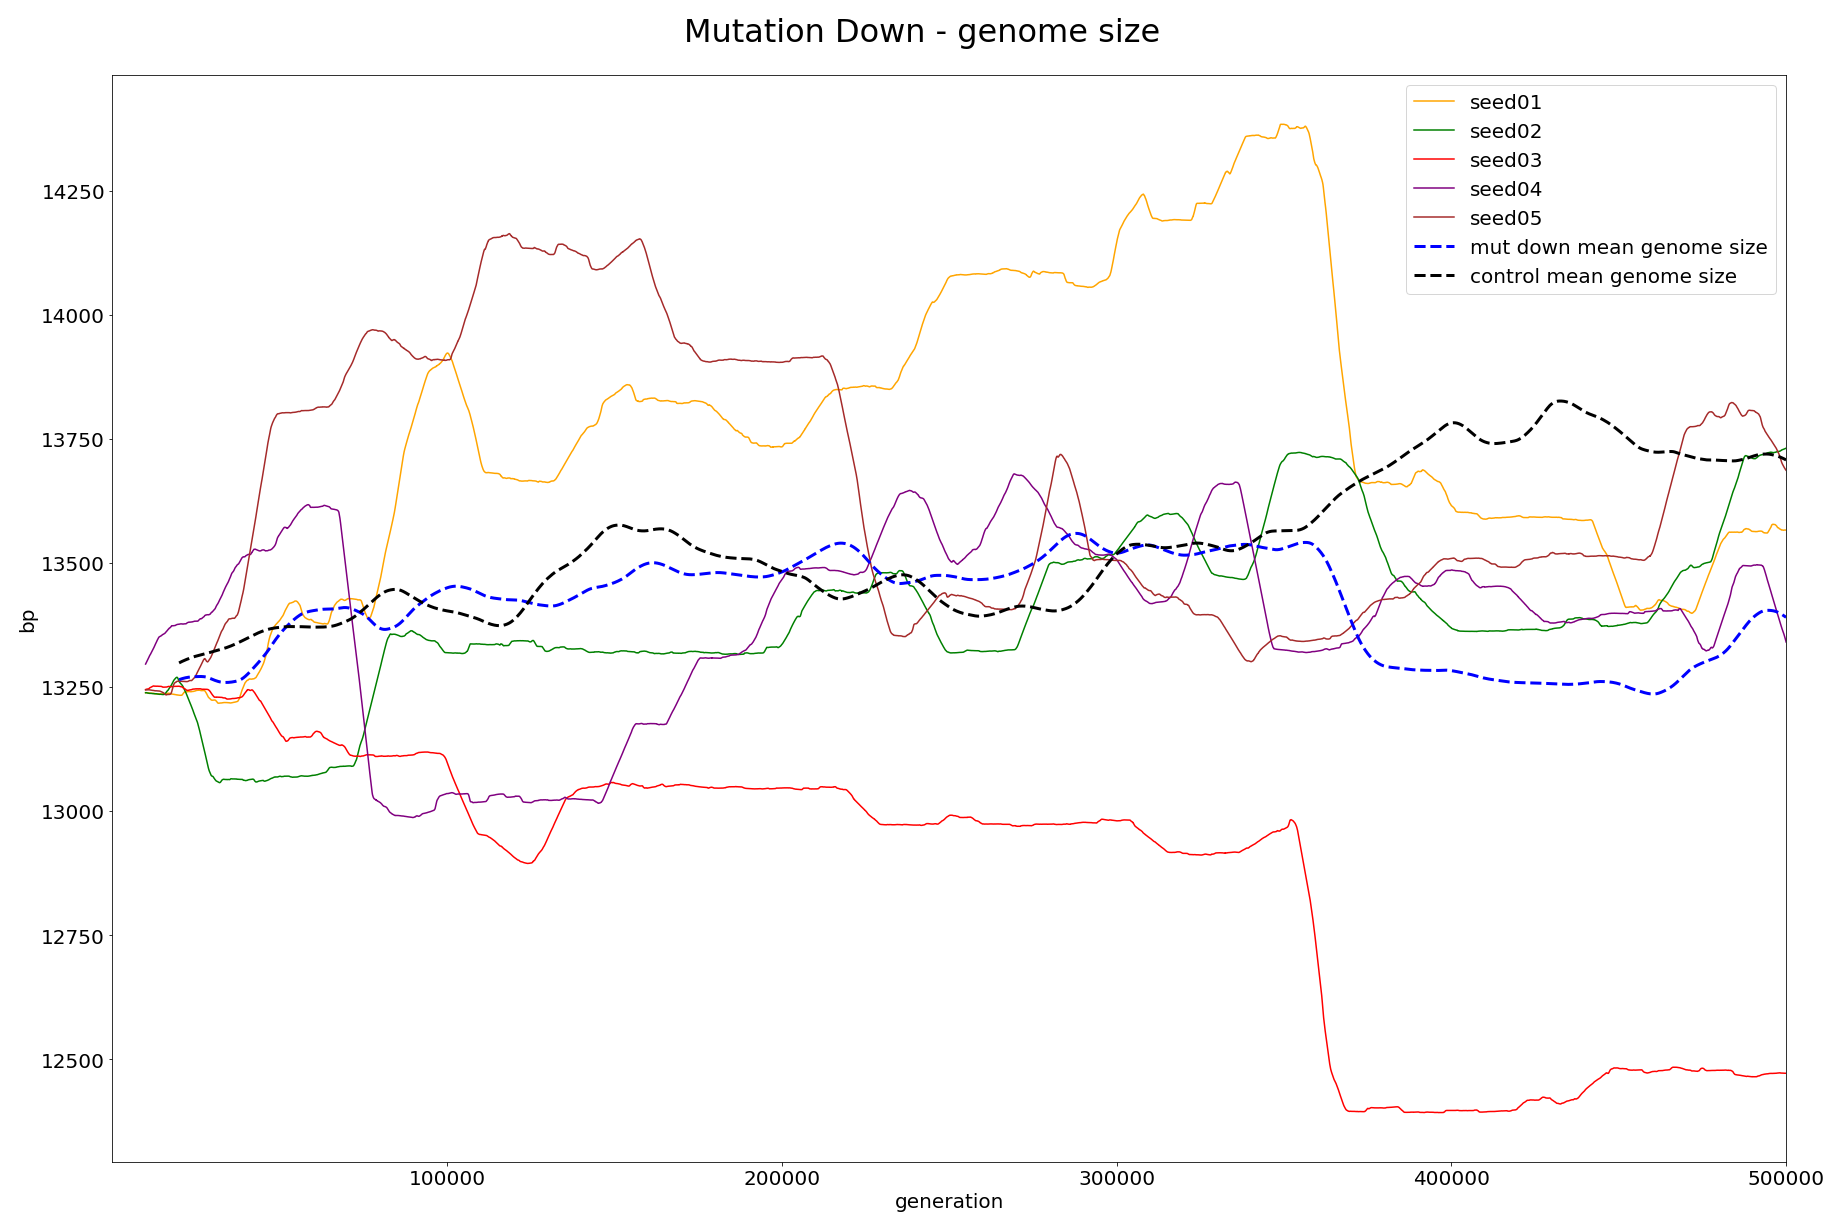
\includegraphics[width=\linewidth]{mut_down_genome_size_b1-e500000}
	\caption[Mutation down genome size]{$\mu_-$ genome size, generations 1-500,000.}
	\label{fig:mut_down:genome_size}
\end{figure}

The well-accepted ``Drake's rule'' states that genome size is inversely proportional to mutation rate~\cite{drake1991constant}. Given the reduced mutation rate of the $\mu_-$ condition, it is expected then that the genome size should increase over the control condition, but this was not the case in these experiments. 

Examining the fitness data in Figure~\ref{fig:mut_down_fitness} it is clear that overall fitness was also not negatively impacted, as one should expect given the lower likelihood of introducing deleterious mutations. 

\begin{figure}[h]
	\centering
	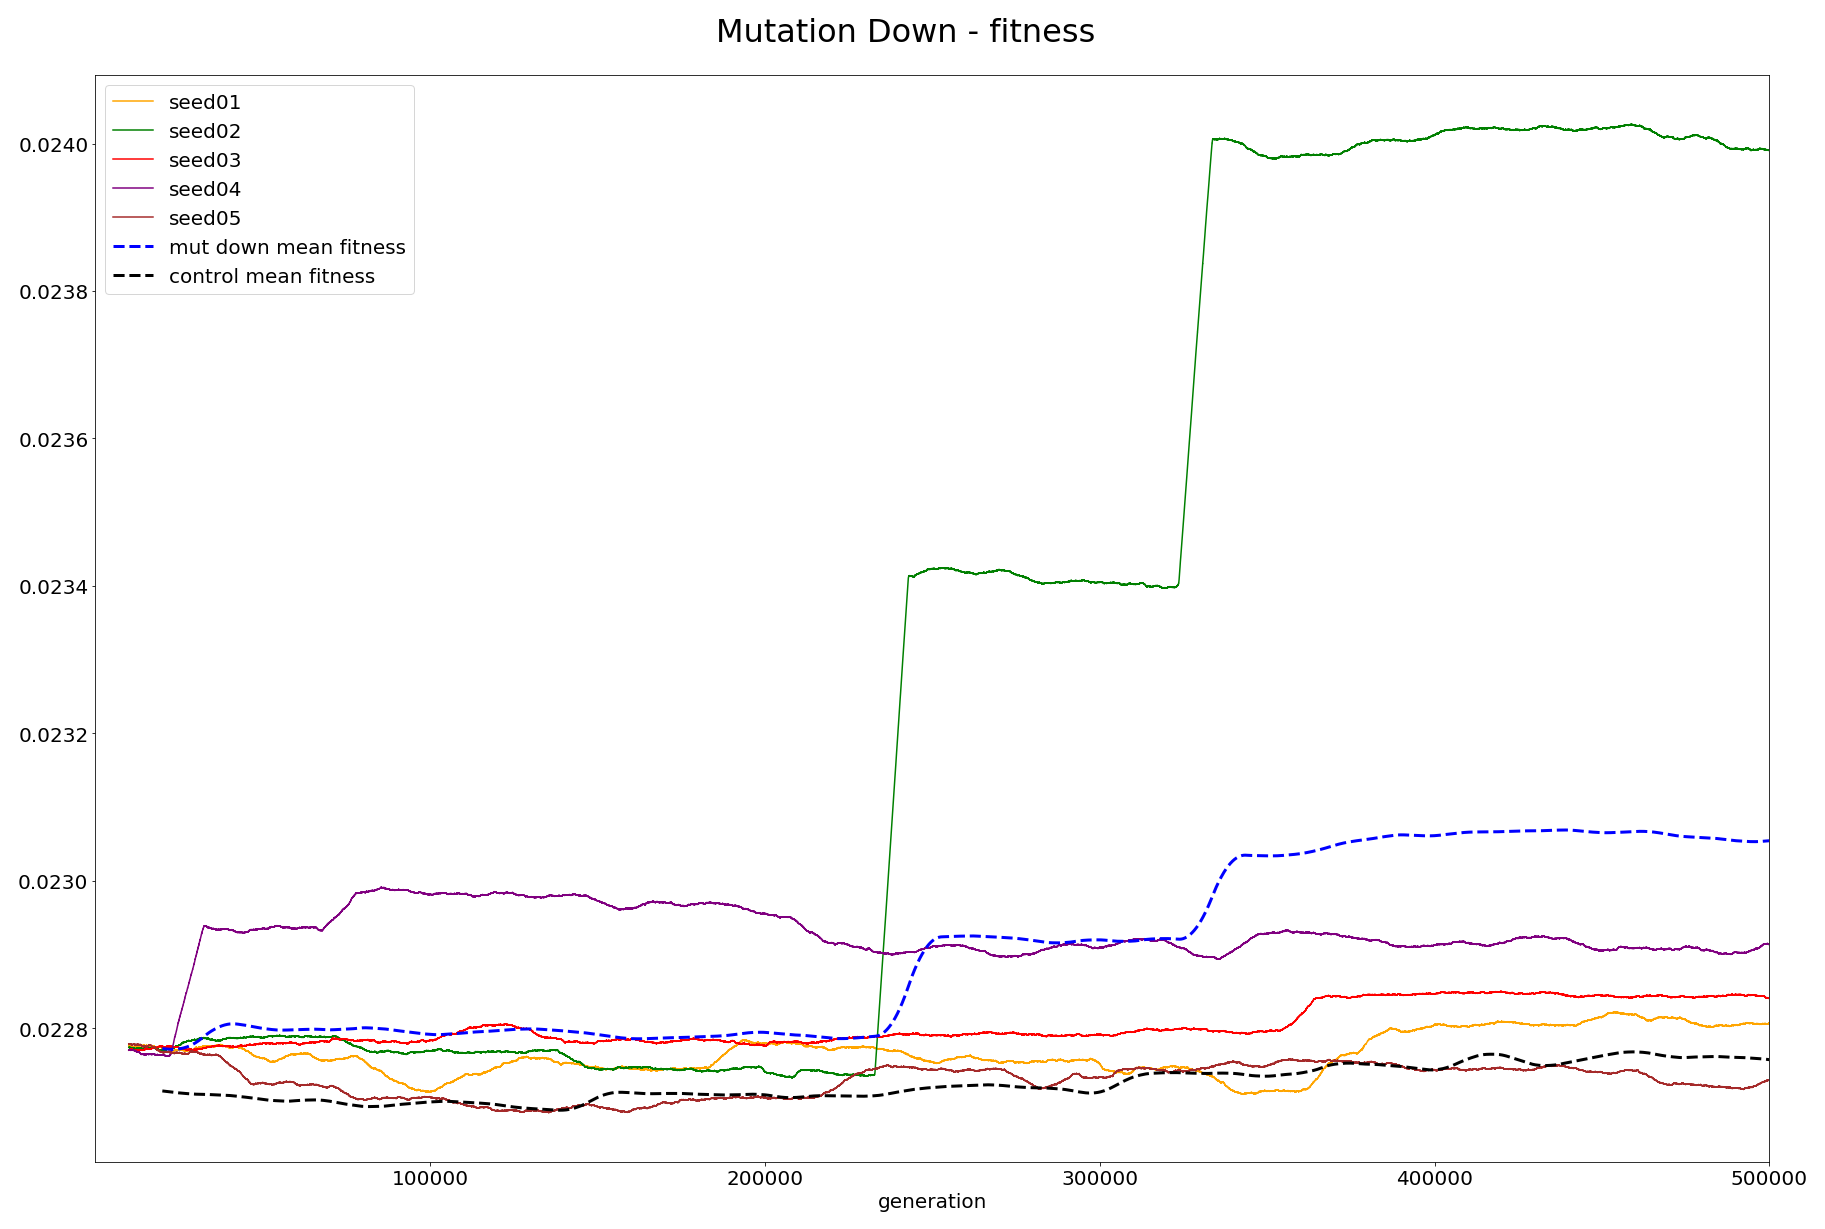
\includegraphics[width=\linewidth]{mut_down_fitness_b1-e500000}
	\caption[Mutation down fitness]{Mutation down population mean fitness, generations 1-500,000, all seeds.}
	\label{fig:mut_down_fitness}
\end{figure} 

Figure~\ref{fig:mut_down_gene_density} shows that gene density significantly increased in the $\mu_-$ condition somewhere around generation 360,000, and this also corresponds to a big bump in fitness, as shown in Figure~\ref{fig:mut_down_fitness} above. 

\begin{figure}[h]
	\centering
	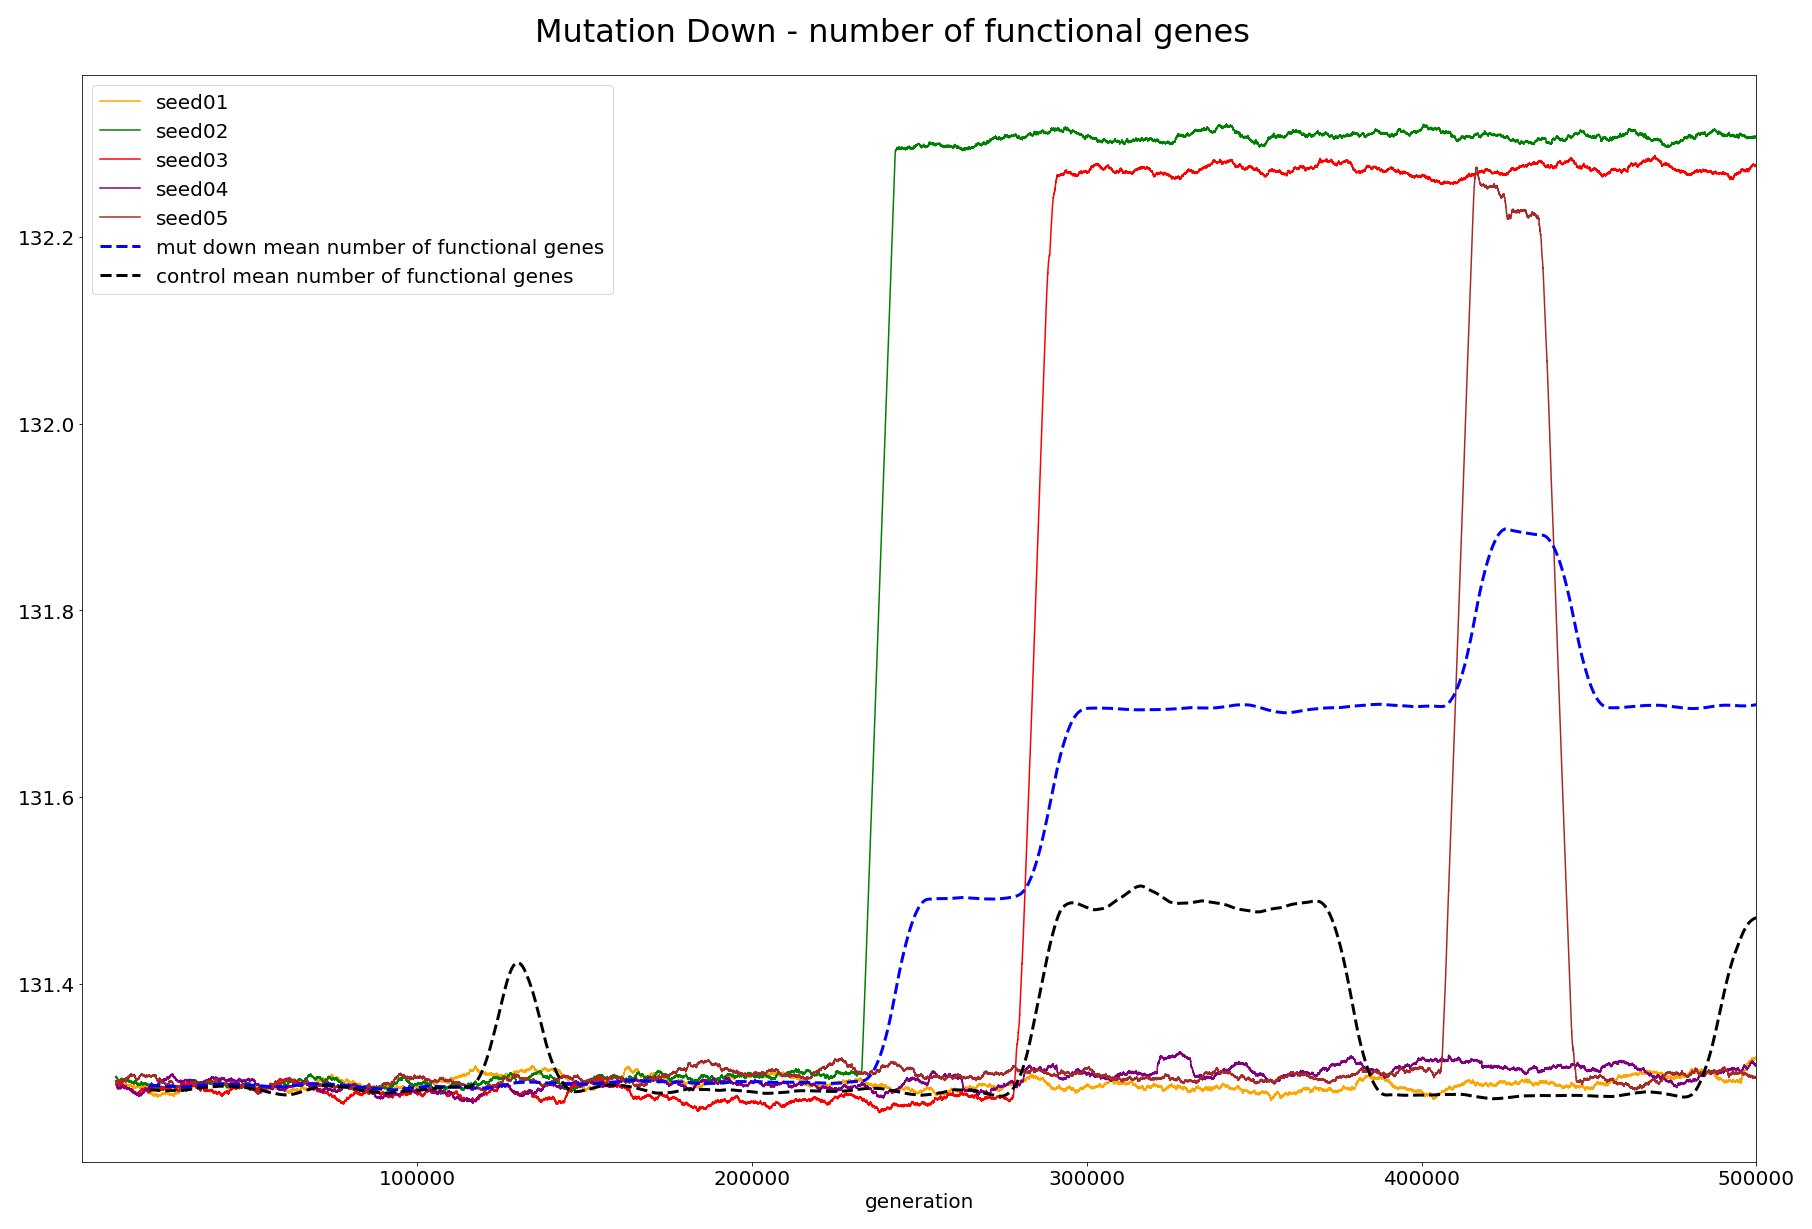
\includegraphics[width=\linewidth]{mut_down_num_functional_genes_b1-e500000}
	\caption[Mutation down number of functional genes]{Mutation down - population mean number of functional genes, generations 1-500,000, all seeds}
	\label{fig:mut_down_num_functional_genes}
\end{figure}

Given the increase in fitness and gene density, and the fact that the number of functional genes increased (see Figure~\ref{fig:mut_down_num_functional_genes} above), it seems clear that, unlike in real populations where the rate of selection may vary dynamically according to several factors \cite{lynch2016genetic}, the steady selection rate of these experiments overcame the natural accumulation of deleterious mutations in favor of a denser genome. The loss of non-coding bases shown in Figure~\ref{fig:mut_down_perc_non-coding} confirm this.

\begin{figure}[h]
	\centering
	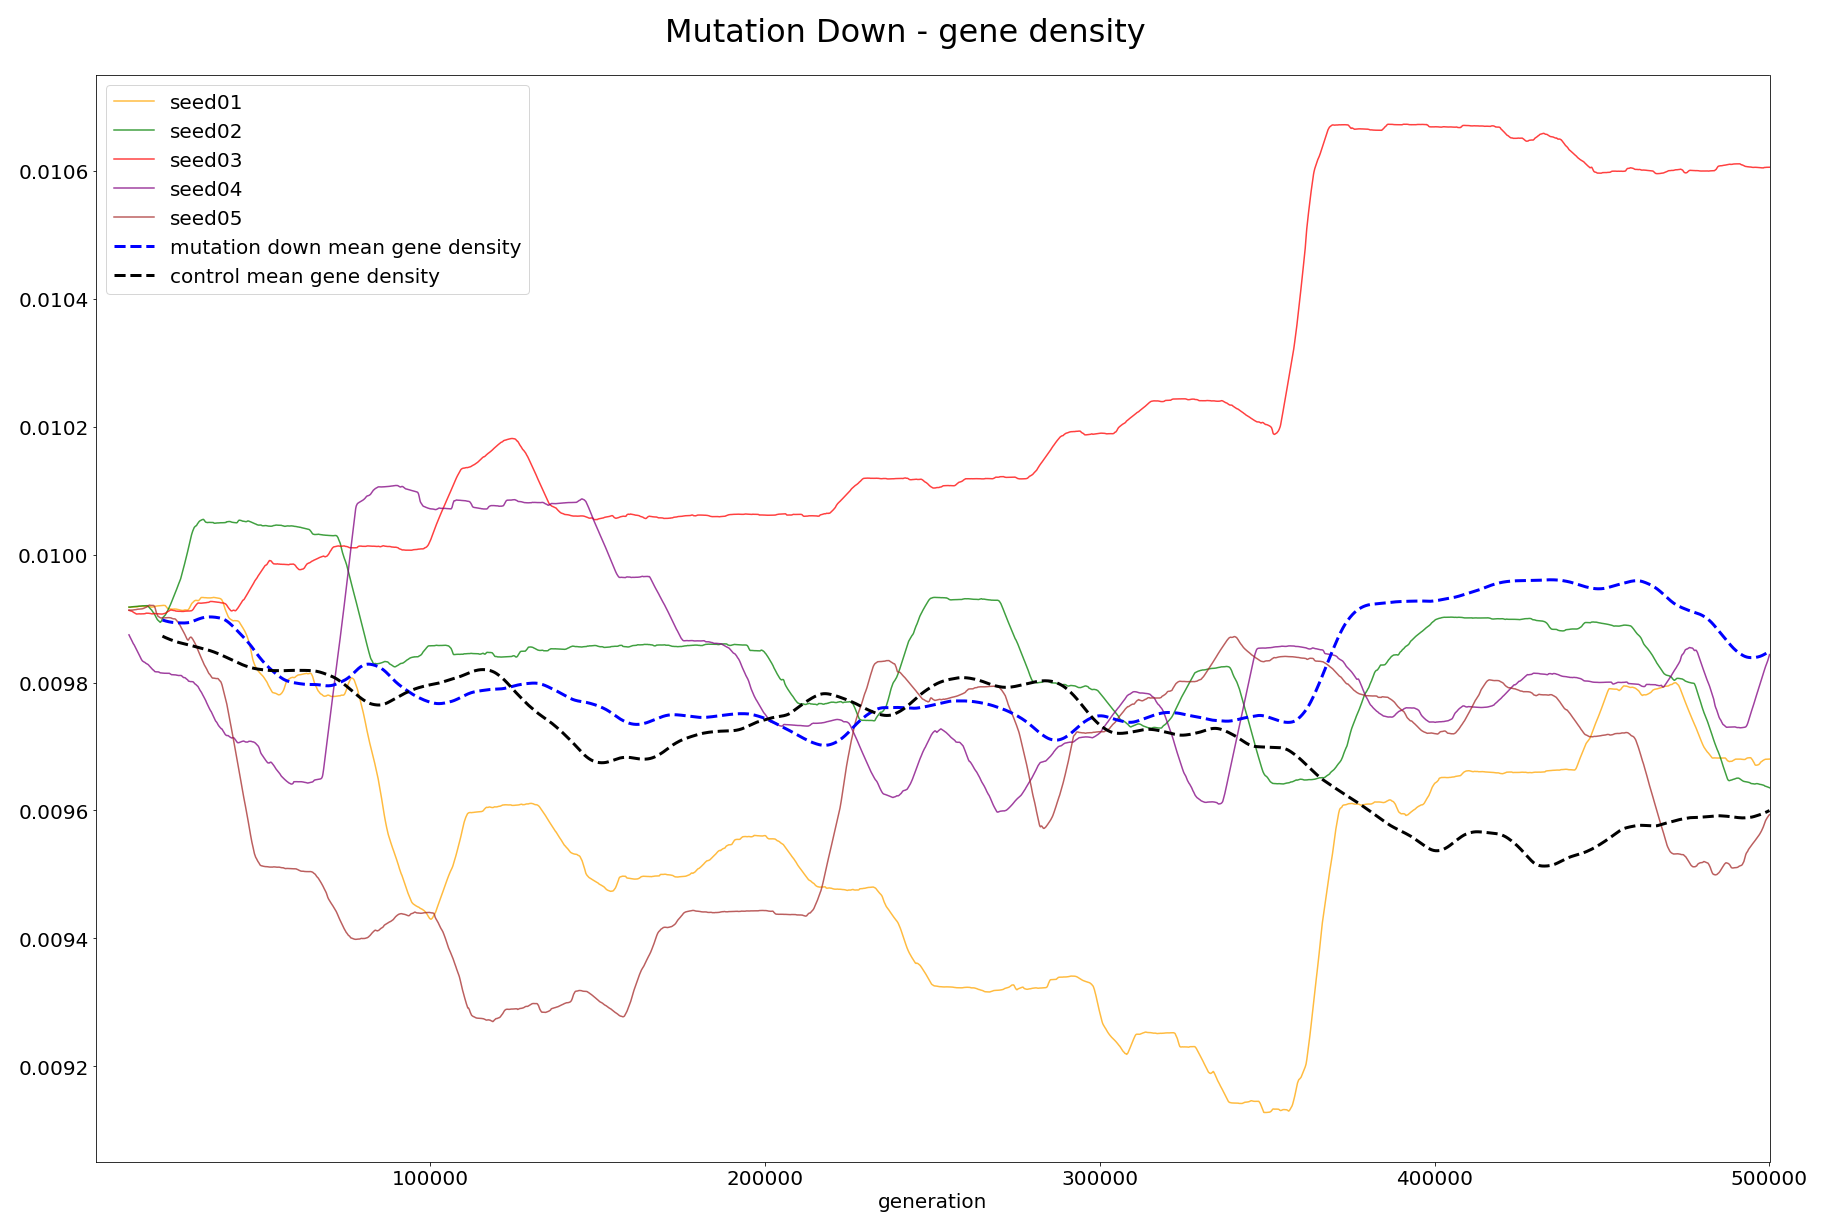
\includegraphics[width=\linewidth]{mut_down_gene_density_b1-e500000}
	\caption[Mutation down gene density]{$\mu_-$ population mean gene density, generations 1-500,000, all seeds.}
	\label{fig:mut_down_gene_density}
\end{figure}


\begin{figure}[h]
	\centering
	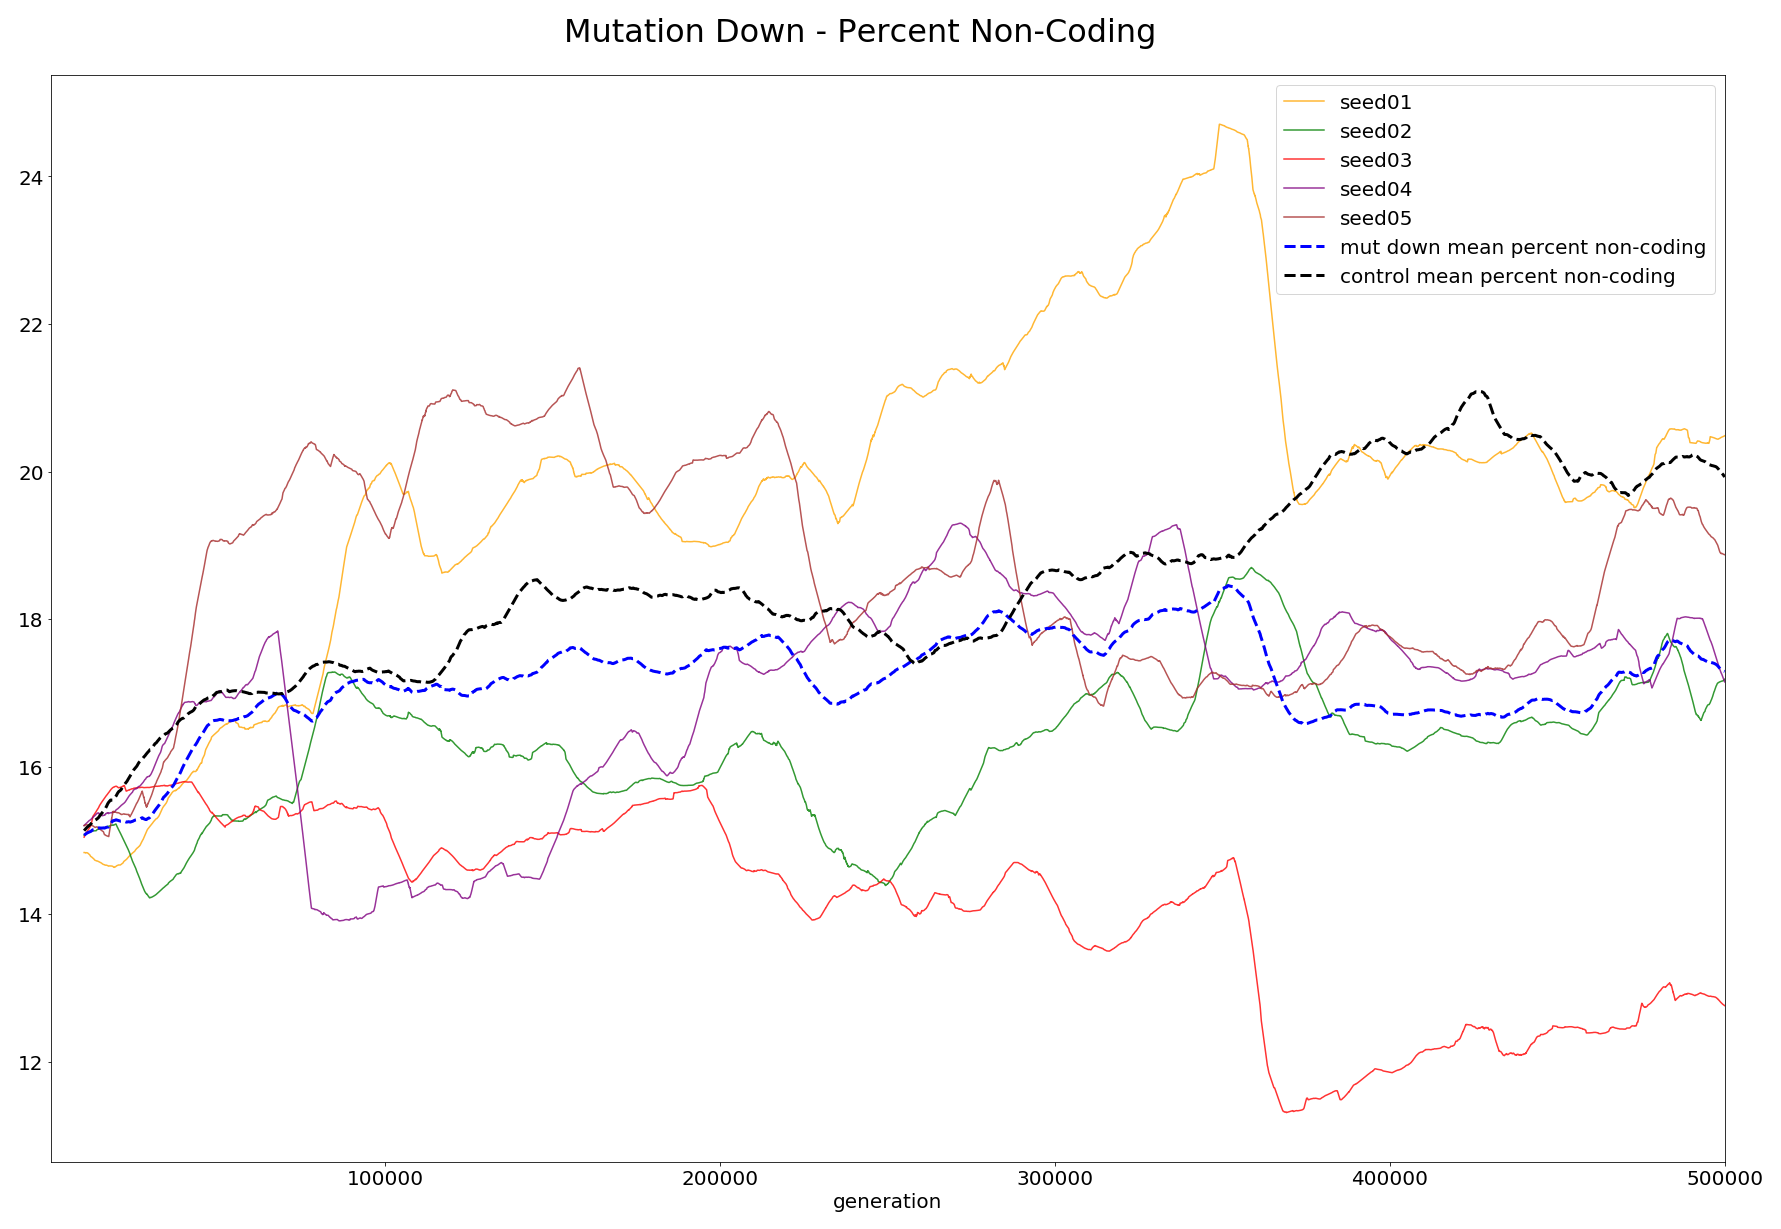
\includegraphics[width=\linewidth]{mut_down_percent_non-coding_b1-e500000}
	\caption[Mutation down percent non-coding]{$\mu_-$ population mean percent non-coding, generations 1-500,000, all seeds.}
	\label{fig:mut_down_perc_non-coding}
\end{figure}


% SELECTION UP
\subsection{Selection Up}
Figure~\ref{fig:selection_up_genome_size} shows that the genome size increased under increased selection, confirming the expected results based on Batut et al.~\cite{Batut.2013}. 
\begin{figure}[H]
	\centering
	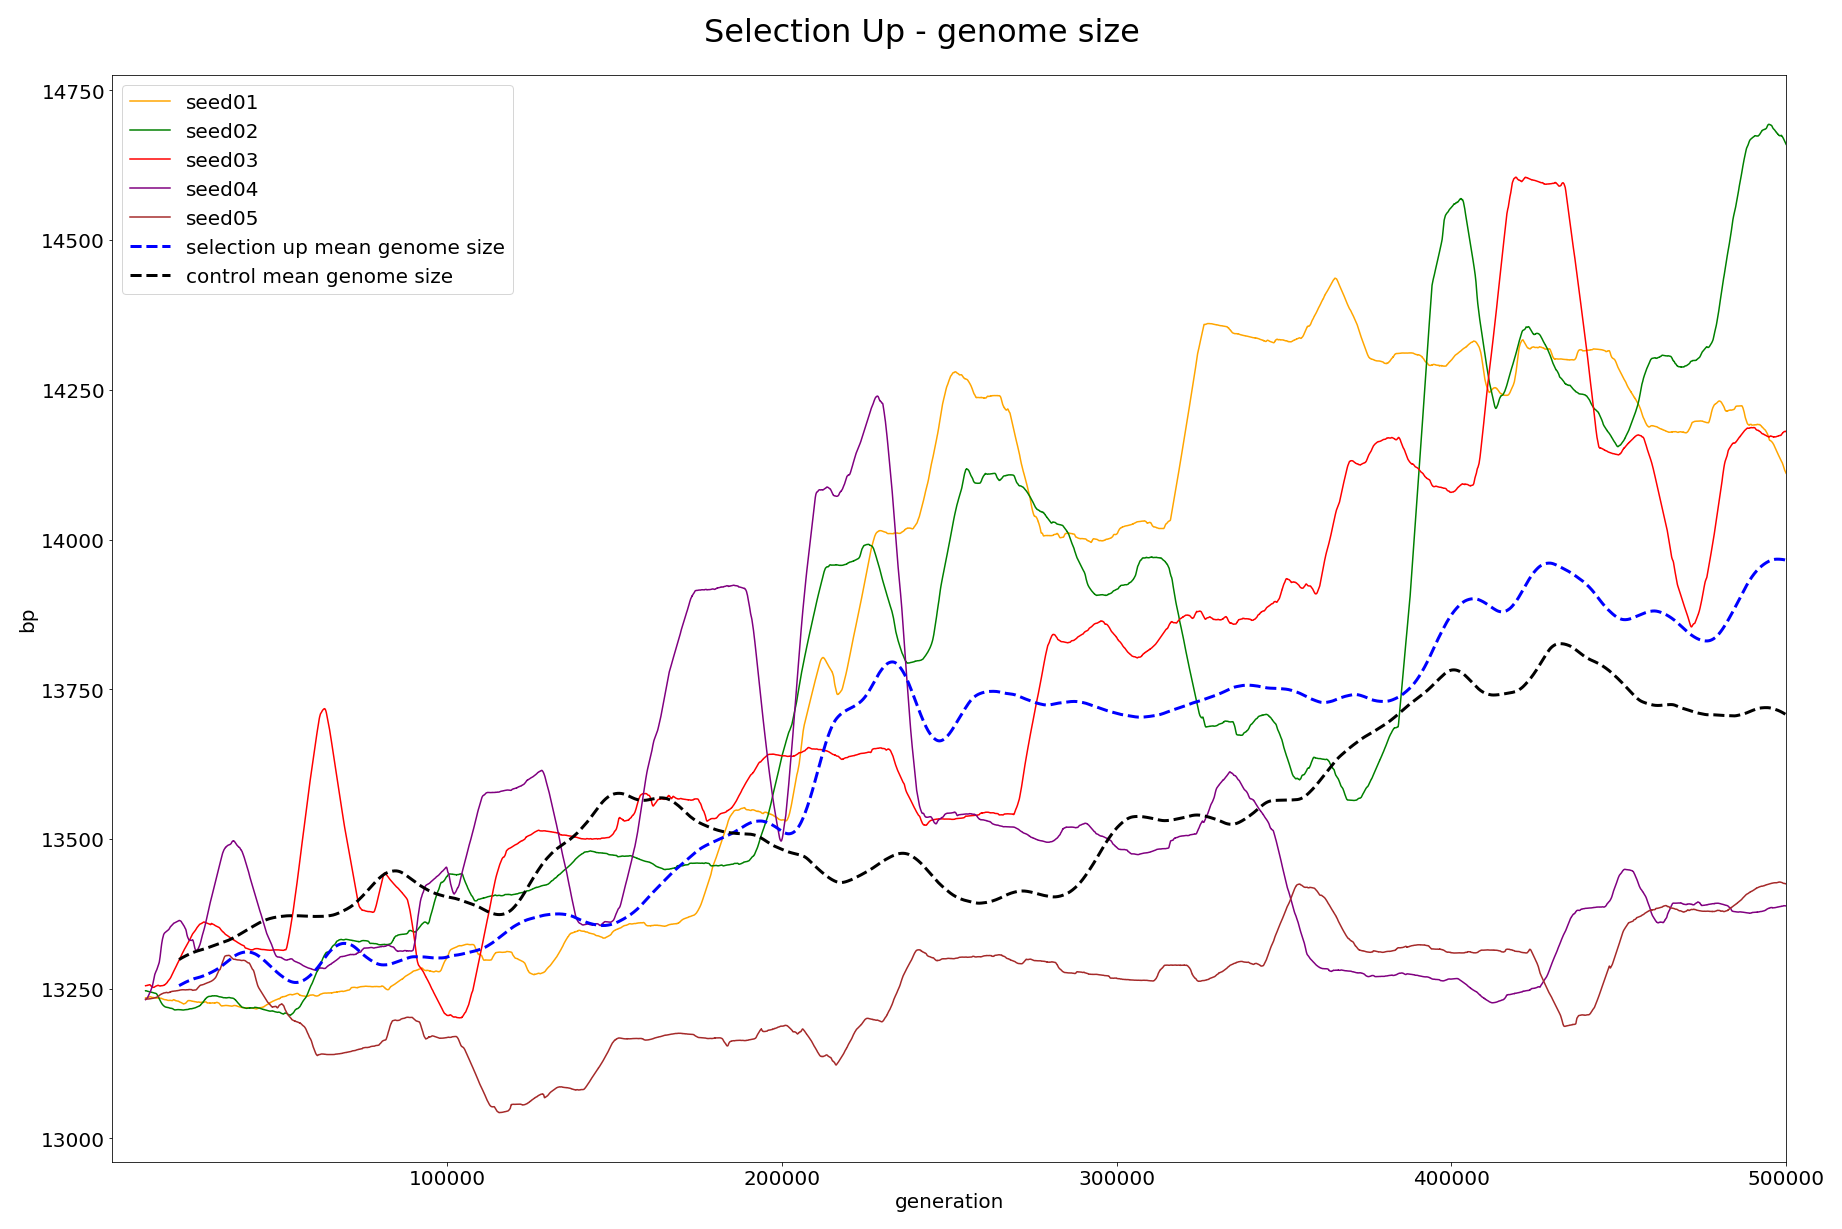
\includegraphics[width=\linewidth]{selection_up_genome_size_b1-e500000}
	\caption[Selection up genome size]{$k_+$ genome size, generations 1-500,000.}
	\label{fig:selection_up_genome_size}
\end{figure}

As with the experiments of Batut et al., the primary gain seems to be in the number of genes, as Figure~\ref{fig:selection_up_num_functional_genes} illustrates. Figure~\ref{fig:selection_up_fitness} shows that fitness overall saw an upward trend, also confirming the results of Batut et al. The large disparity in the fitness scale between the $k_+$ and the control conditions is due to Aevol's \texttt{fitness\_proportionate} selection method. Recall that in the \texttt{fitness\_proportionate} selection method, the probability $p$ of reproduction for an organism with gap $g$ is given by:
\begin{equation*}
p = \frac{e^{-k*g}}{\sum_{i=1}^{N}e^{-k*g_i}}
\end{equation*}
where $g_i$ is the gap for the $i$th organism in the population. Thus, changing the selection parameter $k$, as in the $k_+$ and $k_-$ conditions, changes the scale of the fitness values. Their behavior over time is more important than the scale, but in order to not skew the visualization, the control condition is left off of the fitness plots.

\begin{figure}[h]
	\centering
	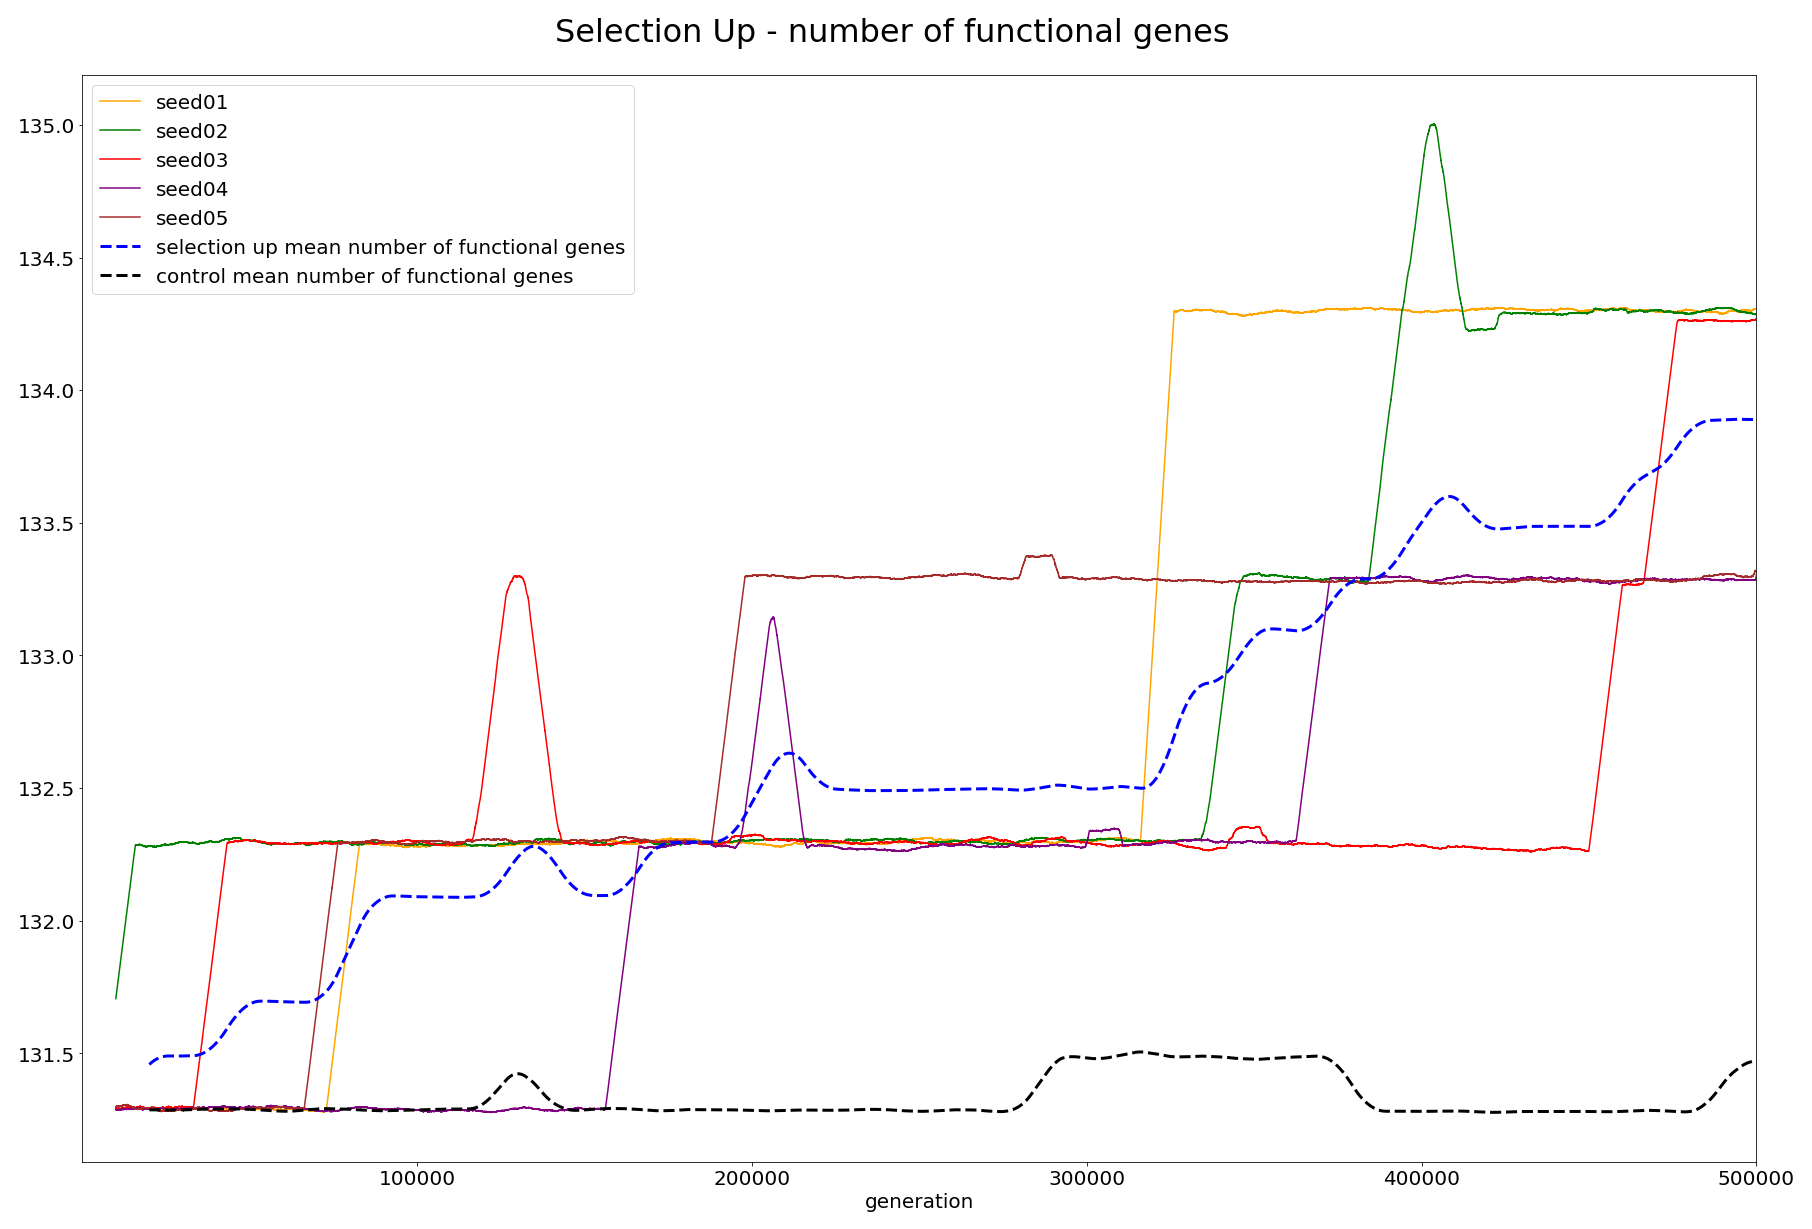
\includegraphics[width=\linewidth]{selection_up_num_functional_genes_b1-e500000}
	\caption[Selection up number of functional genes]{$k_+$ population mean number of functional genes, generations 1-500,000, all seeds.}
	\label{fig:selection_up_num_functional_genes}
\end{figure}

\begin{figure}[h]
	\centering
	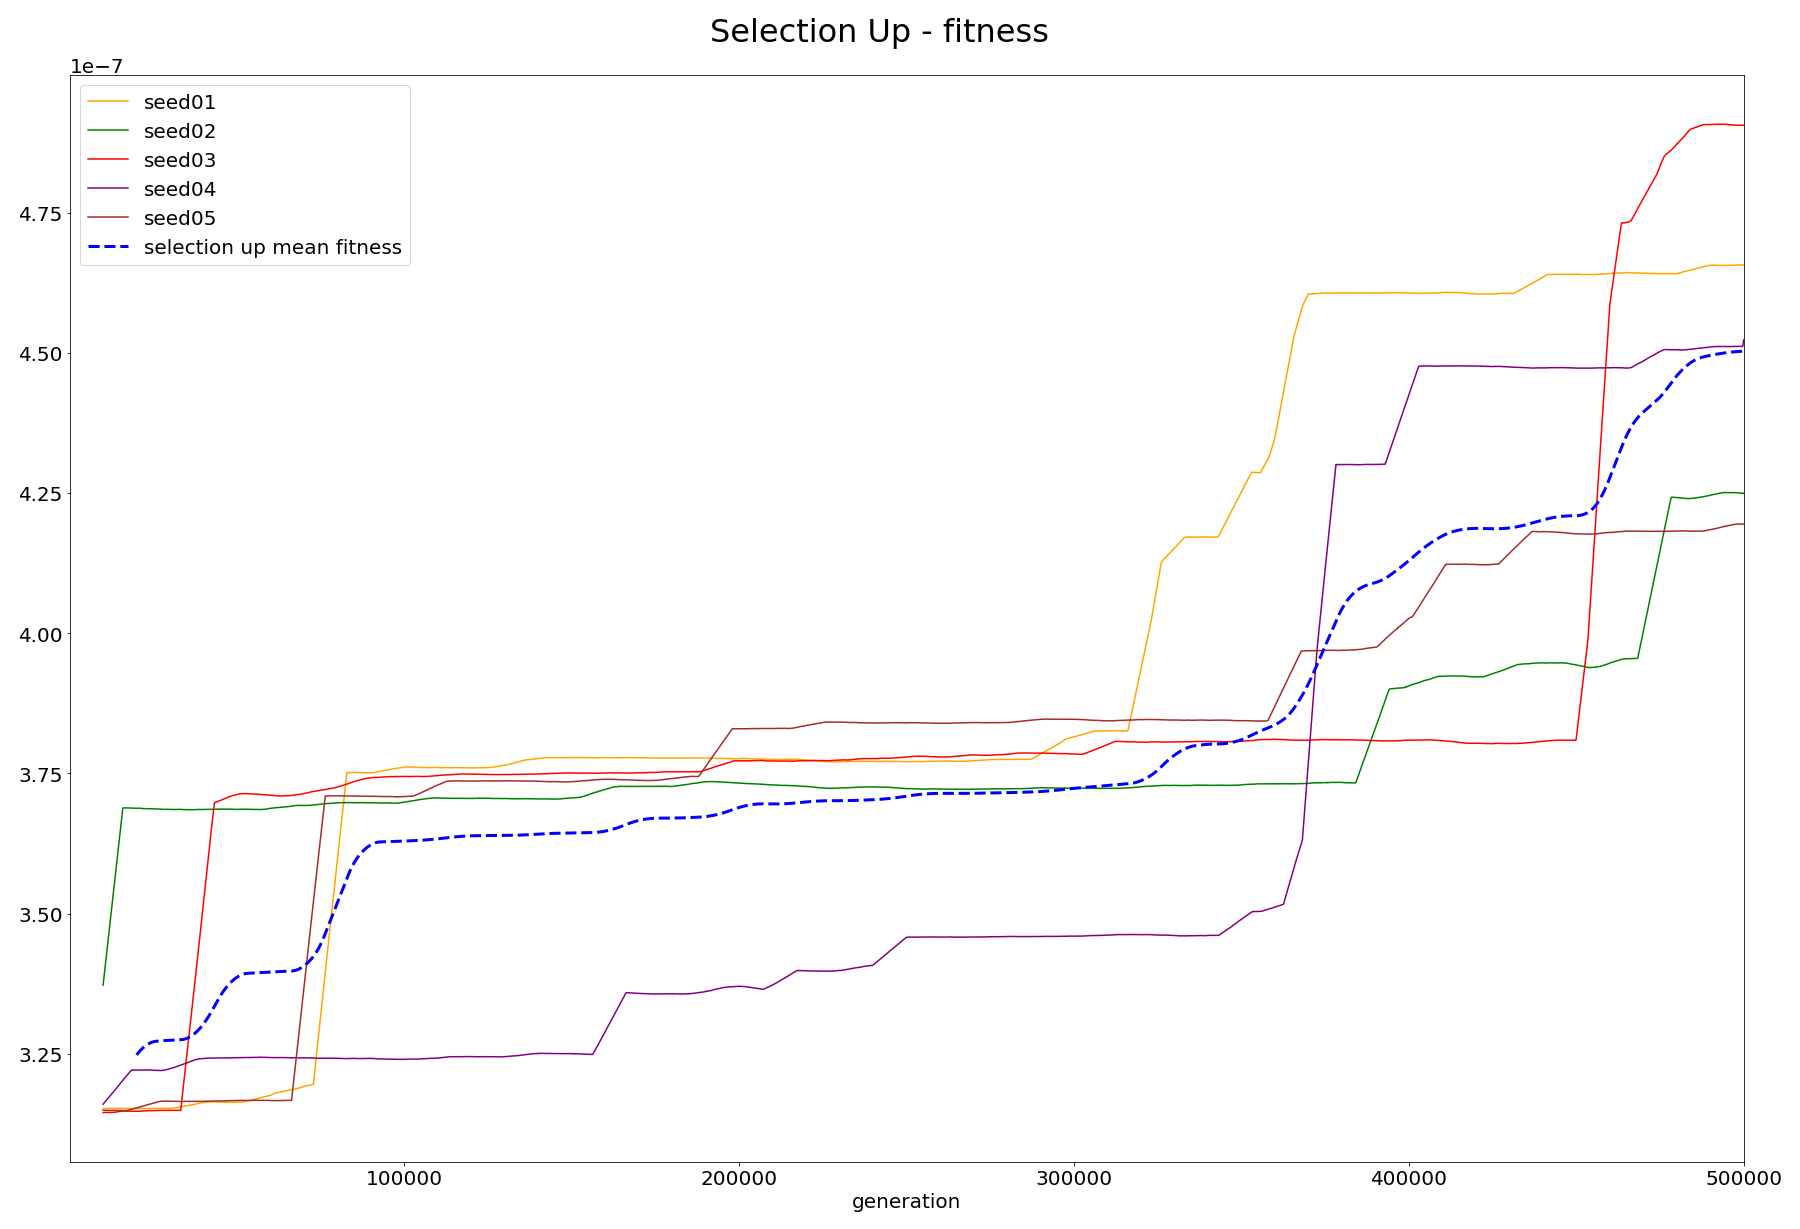
\includegraphics[width=\linewidth]{selection_up_fitness_b1-e500000}
	\caption[Selection up fitness]{$k_+$ population mean fitness, generations 1-500,000, all seeds.}
	\label{fig:selection_up_fitness}
\end{figure}

Lastly, Figure~\ref{fig:selection_up_perc_non-coding} shows that some of the increased genome size is due to addition of non-coding bases, too. 

\begin{figure}[h]
	\centering
	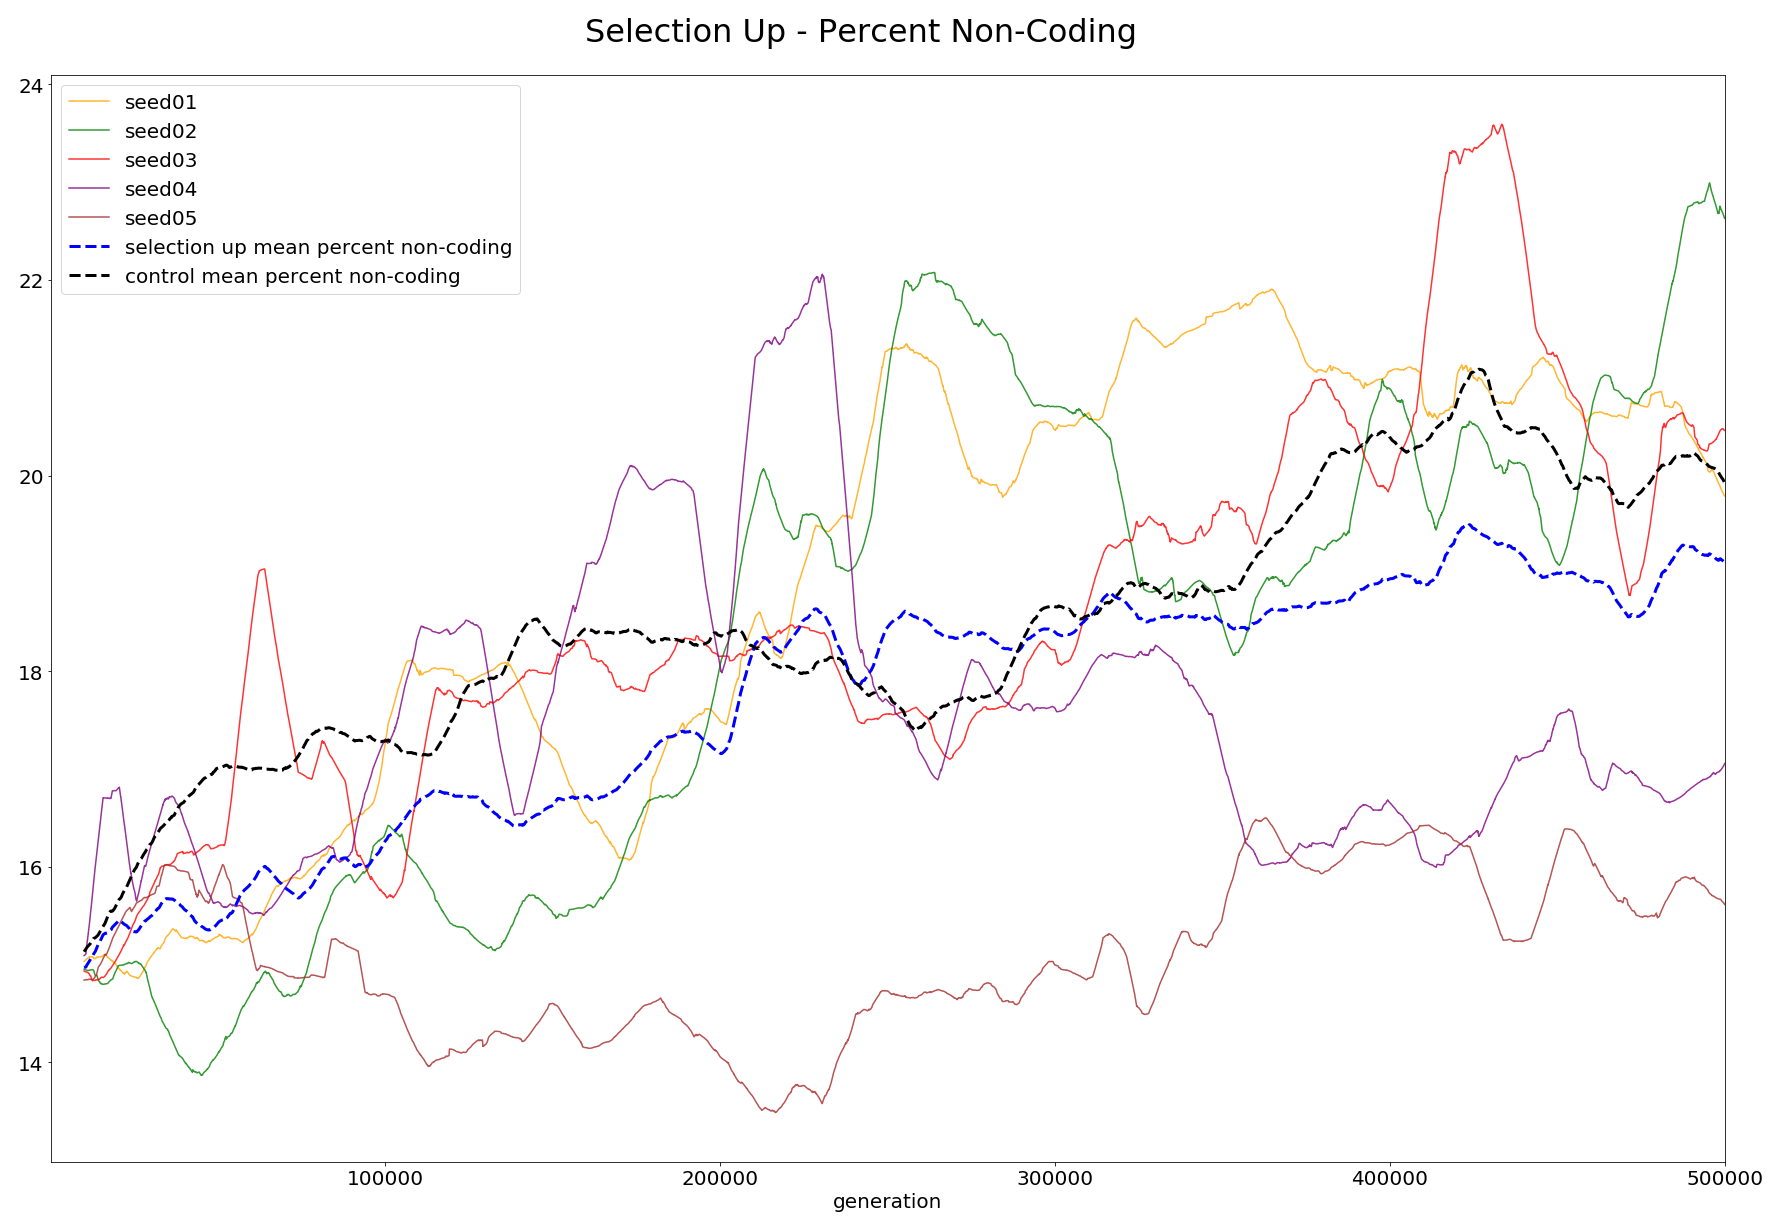
\includegraphics[width=\linewidth]{selection_up_percent_non-coding_b1-e500000}
	\caption[Selection up percent non-coding]{$k_+$ population mean percent non-coding, generations 1-500,000, all seeds.}
	\label{fig:selection_up_perc_non-coding}
\end{figure}
% SELECTION DOWN
\subsection{Selection Down}
Figure~\ref{fig:selection_down_genome_size} shows the genome size results for the $k_-$ condition. 
\begin{figure}[H]
	\centering
	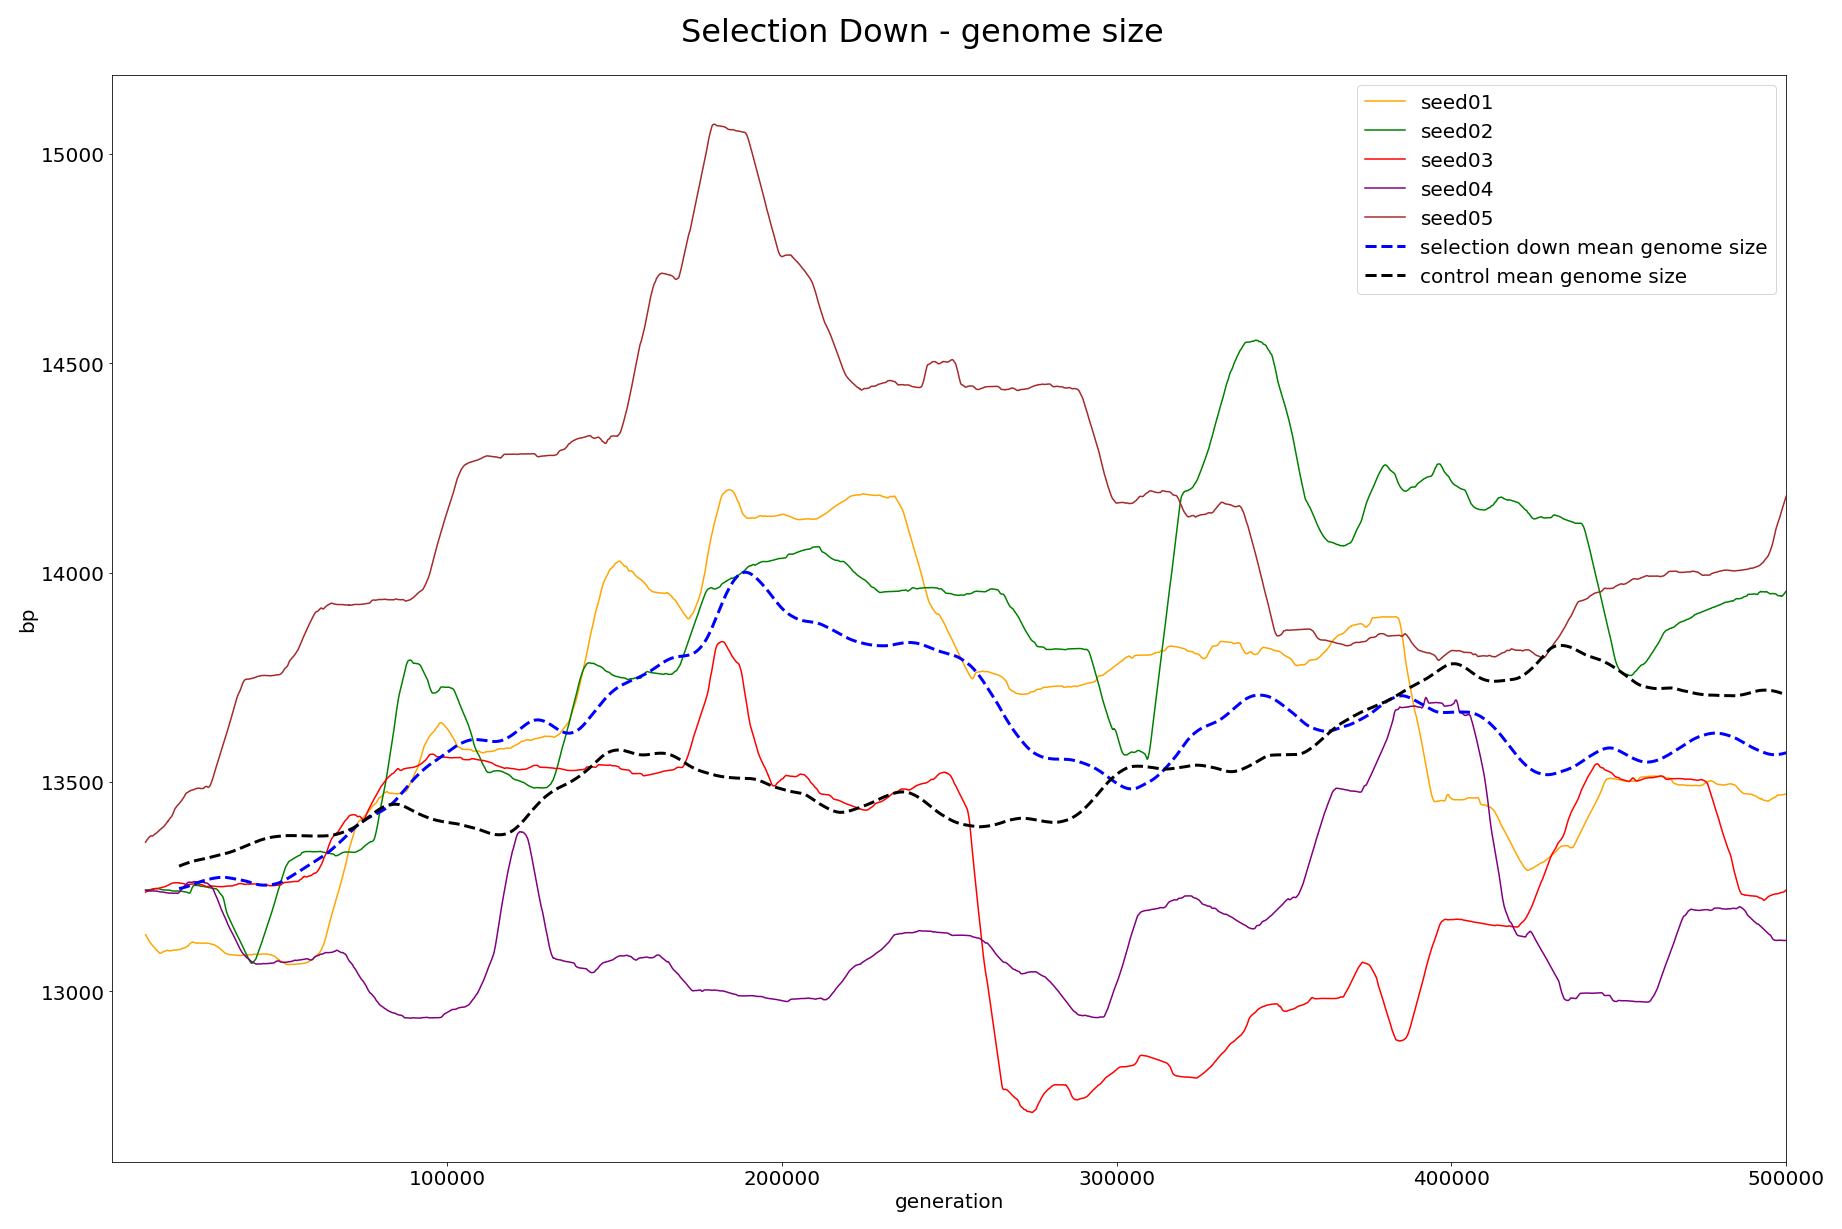
\includegraphics[width=\linewidth]{selection_down_genome_size_b1-e500000}
	\caption[Selection down genome size]{$k_-$ population mean genome size, generations 1-500,000.}
	\label{fig:selection_down_genome_size}
\end{figure}
The slight increase in genome size is probably best explained by the gaining of some non-coding bases, as shown in Figure~\ref{fig:selection_down_perc_non-coding}, as the decreased selection caused an overall loss in the number of functional genes for most seeds for most of the generations (see Figure~\ref{fig:selection_down_num_functional_genes}).  
\begin{figure}[h]
	\centering
	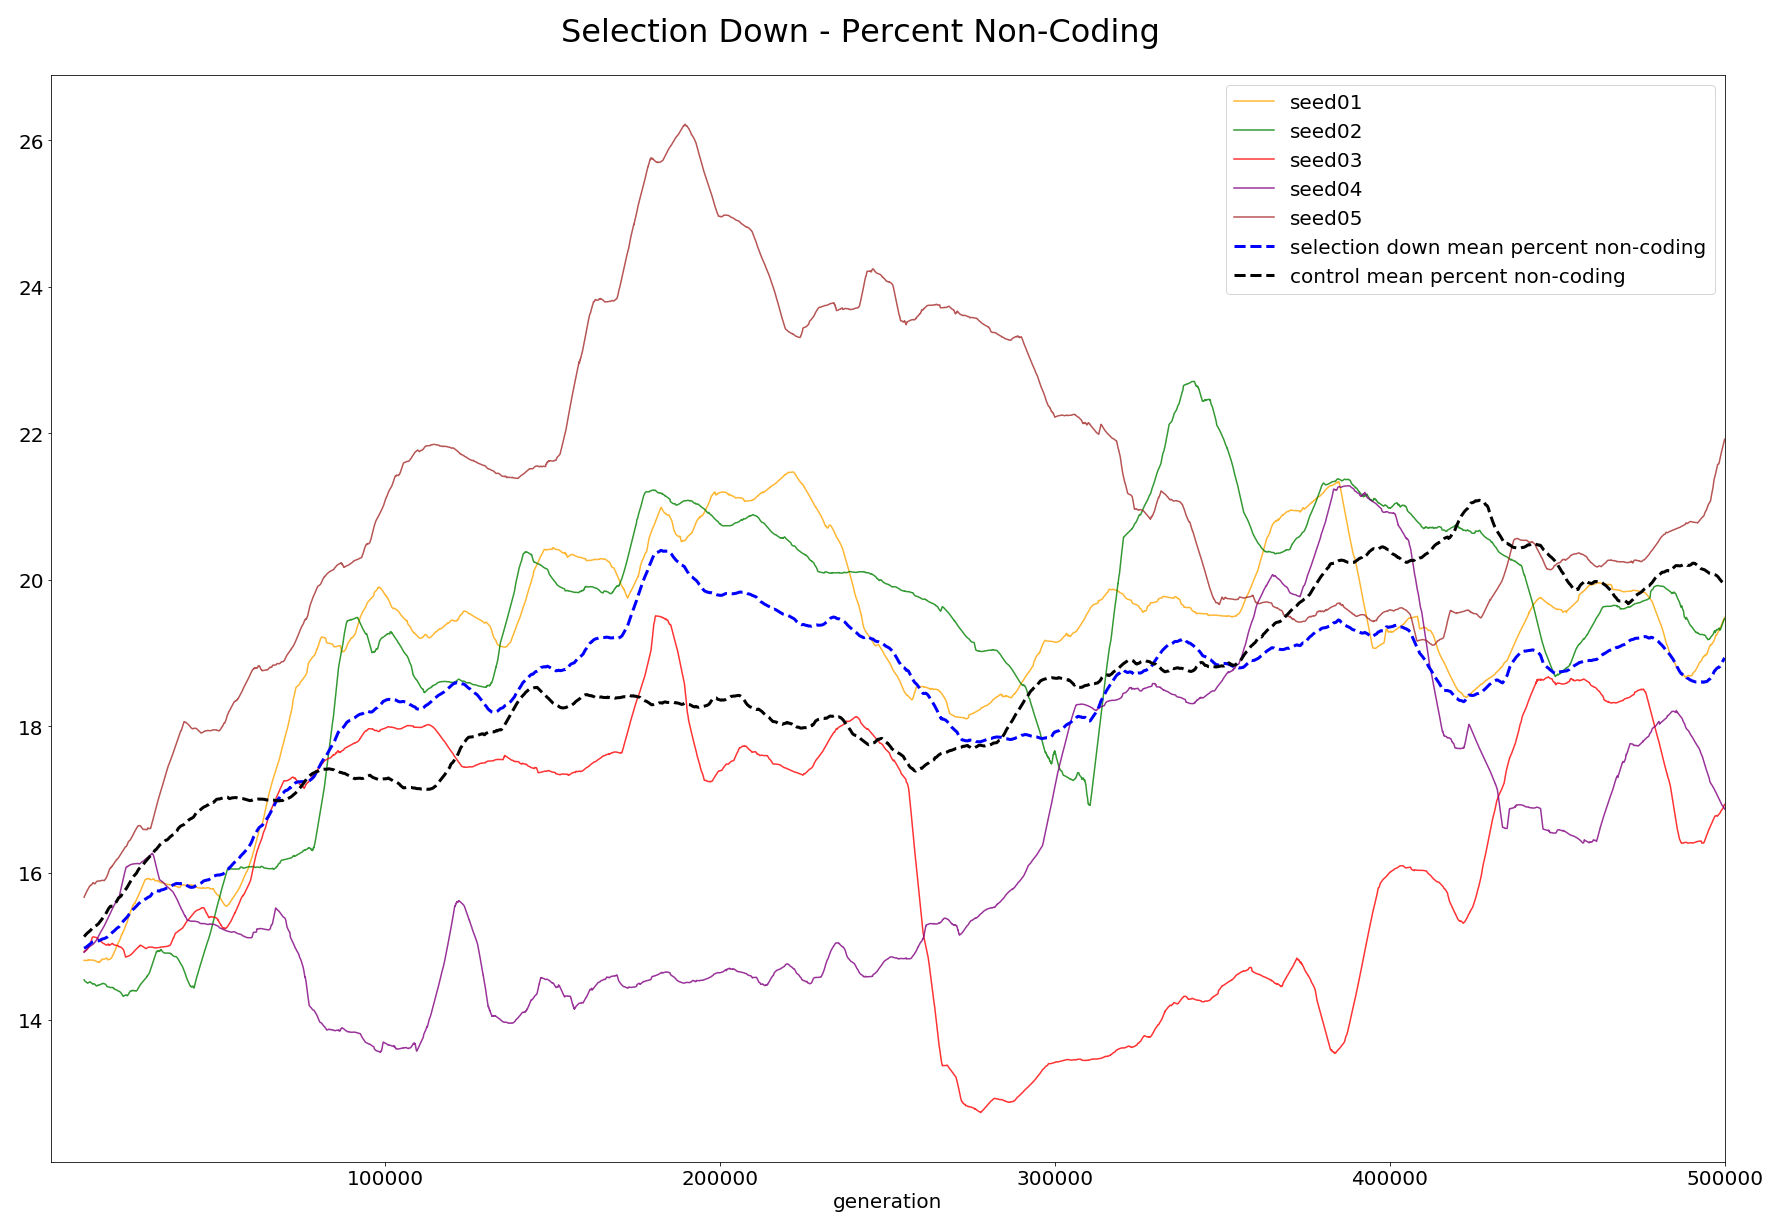
\includegraphics[width=\linewidth]{selection_down_percent_non-coding_b1-e500000}
	\caption[Selection down percent non-coding]{$k_-$ percent non-coding, generations 1-500,000, all seeds.}
	\label{fig:selection_down_perc_non-coding}
\end{figure}

\begin{figure}[h]
	\centering
	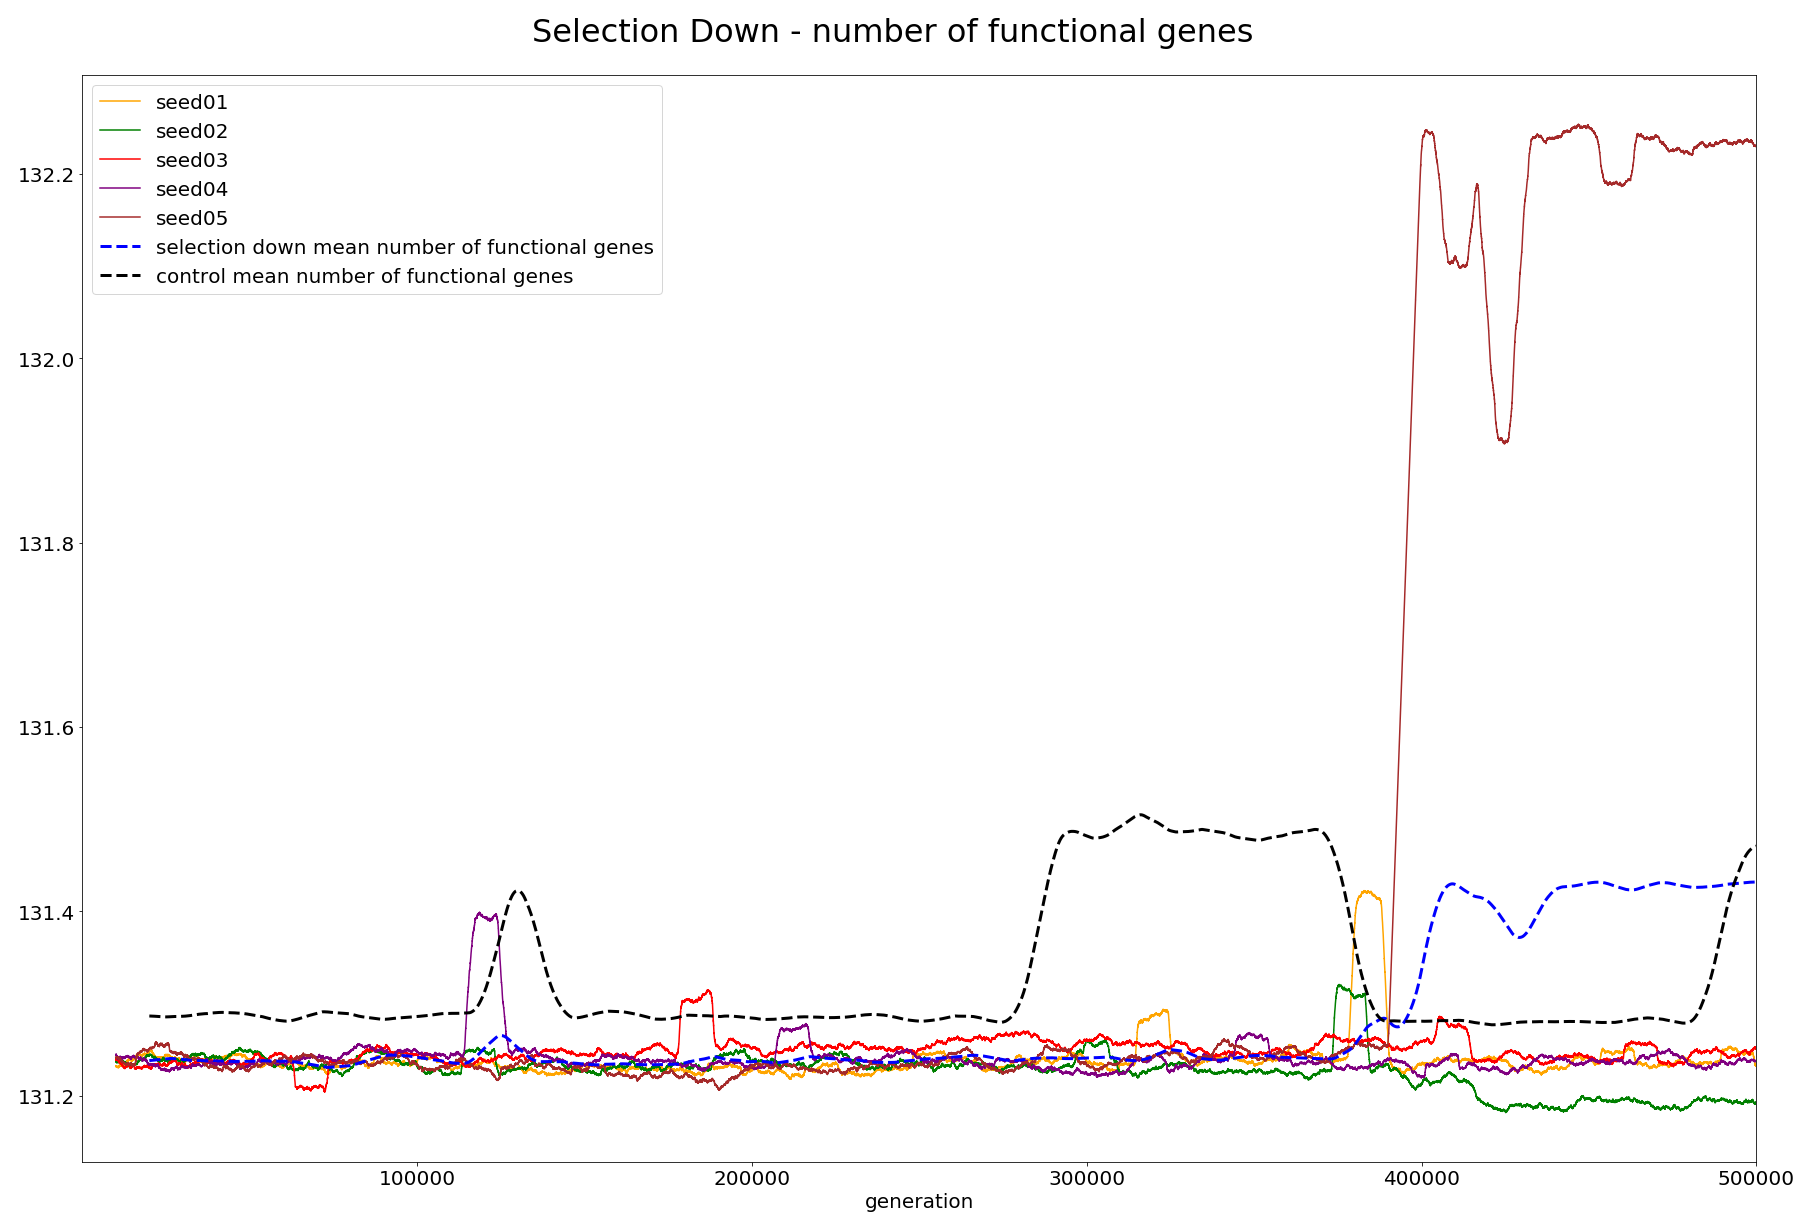
\includegraphics[width=\linewidth]{selection_down_num_functional_genes_b1-e500000}
	\caption[Selection down number of functional genes.]{$k_-$ mean population number of functional genes, generations 1-500,000, all seeds.}
	\label{fig:selection_down_num_functional_genes}
\end{figure}


% POPULATION UP
\subsection{Population Up}
Figure~\ref{fig:pop_up_genome_size} shows the mean population genome size for the $N_+$ condition, and it is clearly the condition which experienced the largest amount of reductive evolution over the course of the 500,000 generations. 
\begin{figure}[h]
	\centering
	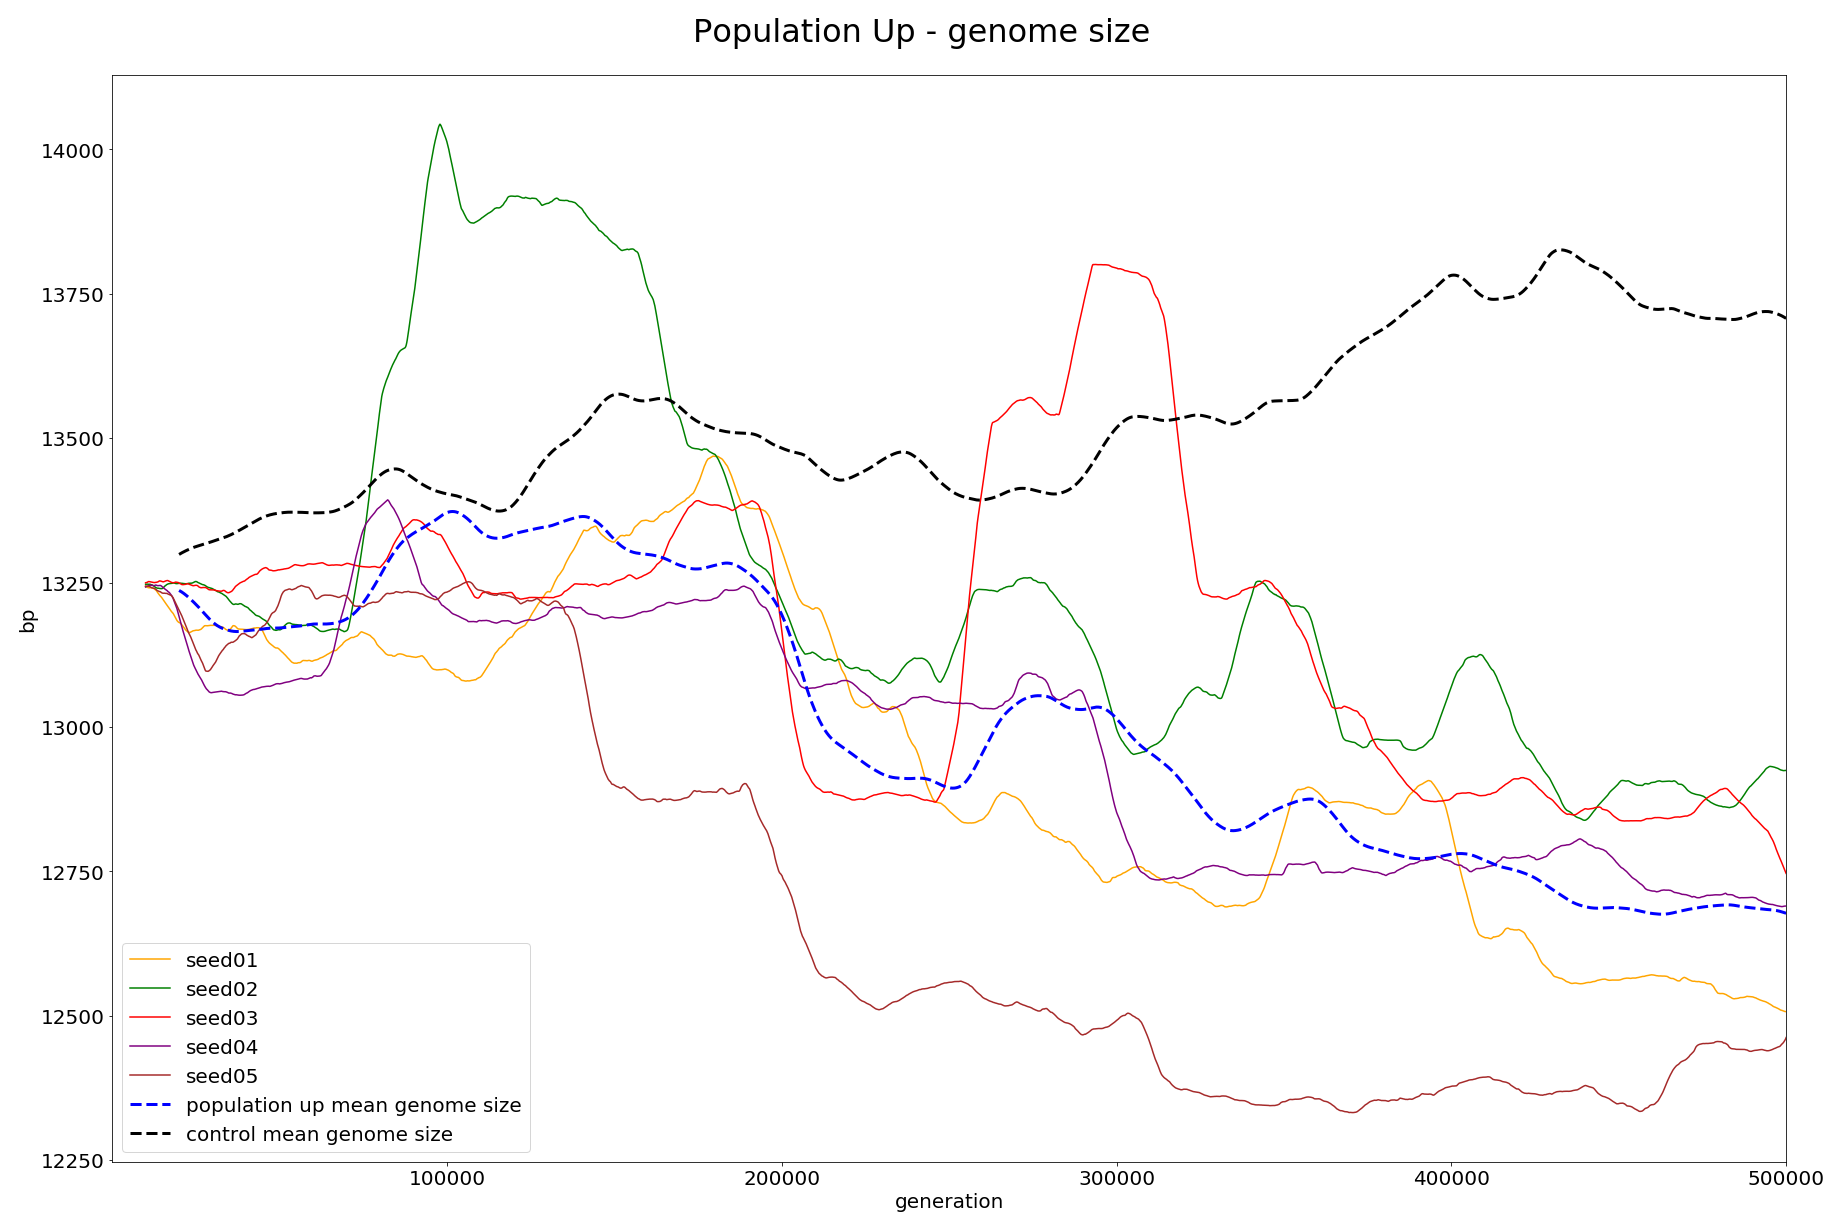
\includegraphics[width=\linewidth]{population_up_genome_size_b1-e500000}
	\caption[Population up genome size]{$N_+$ genome size, generations 1-500,000.}
	\label{fig:pop_up_genome_size}
\end{figure}

Confirming the work of Batut et al.~\cite{Batut.2014}, the increased $N_e$ allowed the efficacy of selection to increase, removing deleterious mutations from the genome, removing non-coding DNA (Figure~\ref{fig:pop_up_perc_non-coding}). 

\begin{figure}[h]
	\centering
	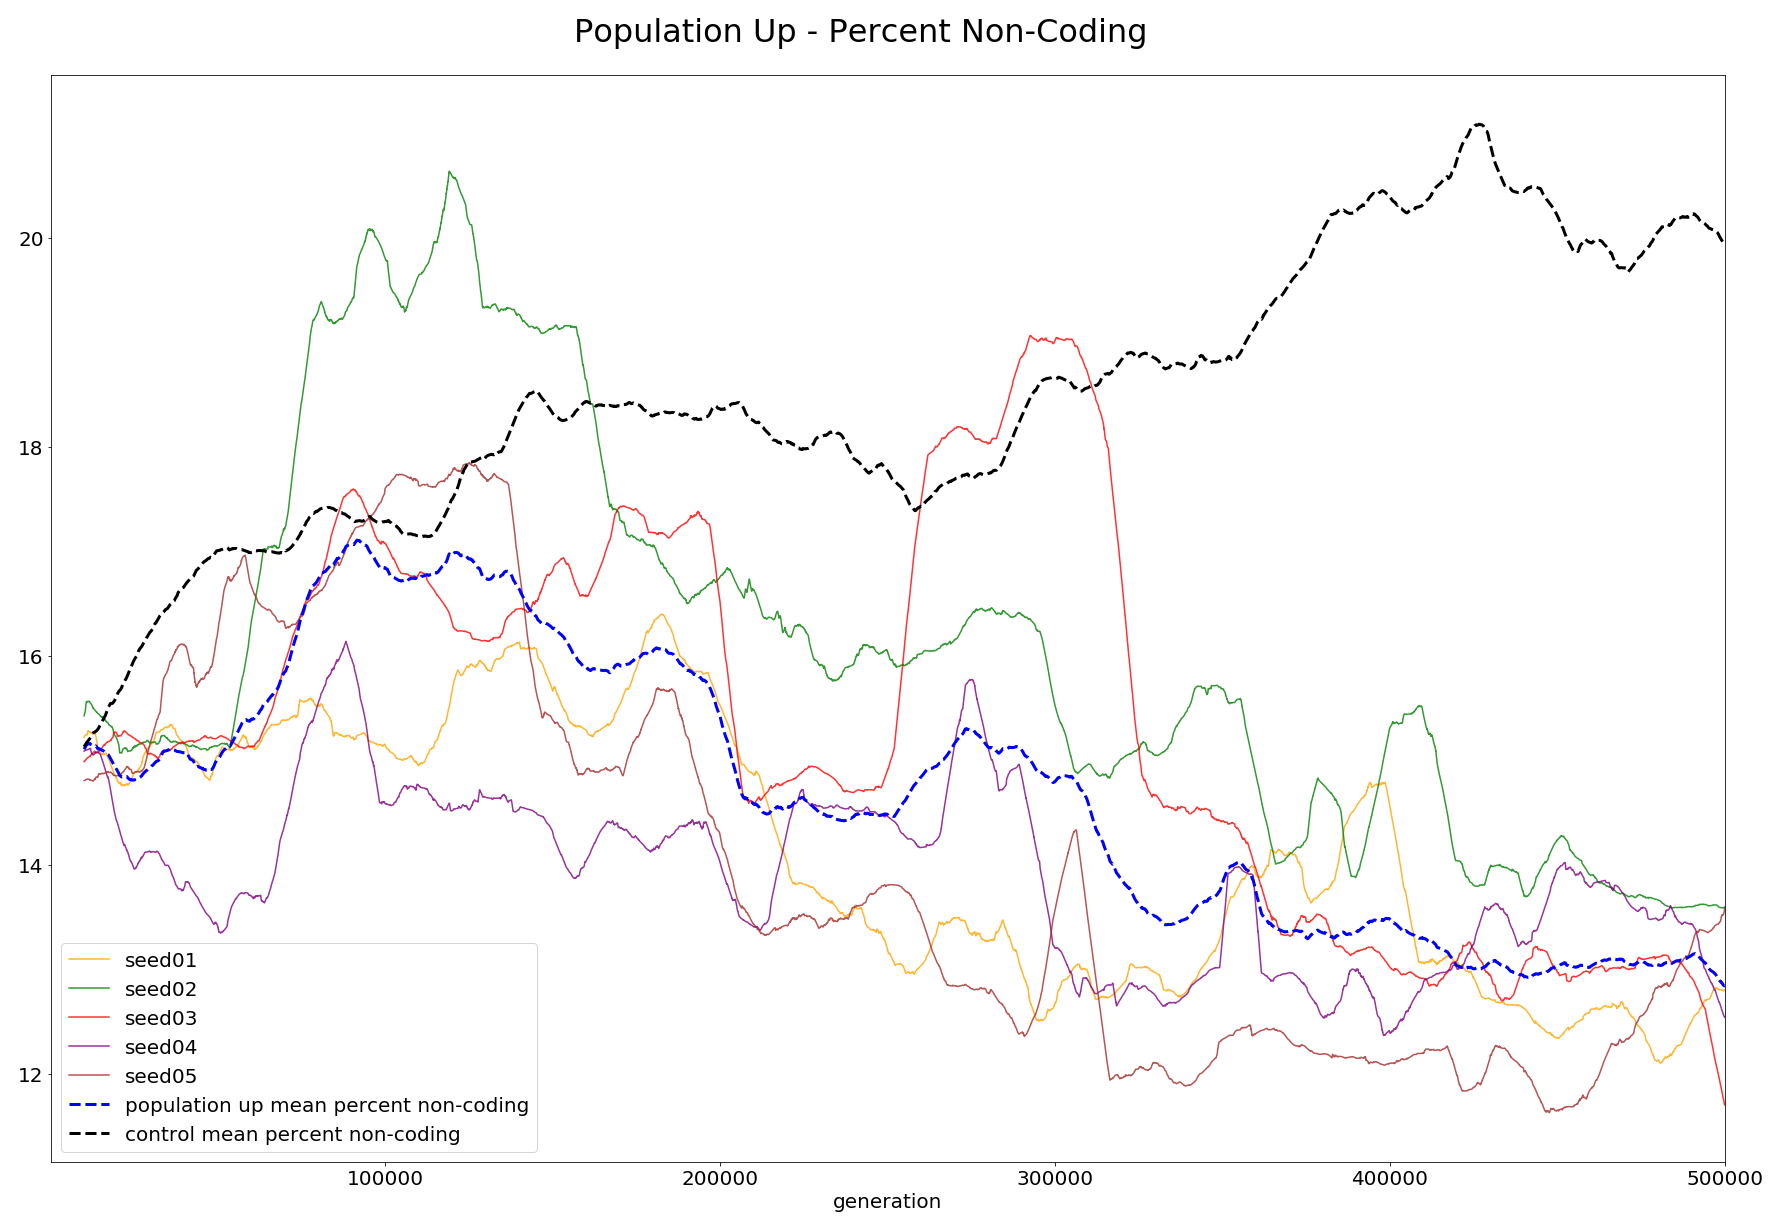
\includegraphics[width=\linewidth]{population_up_percent_non-coding_b1-e500000}
	\caption[Population up percent non-coding]{$N_+$ population mean percent non-coding, generations 1-500,000, all seeds.}
	\label{fig:pop_up_perc_non-coding}
\end{figure}



% POPULATION DOWN
\subsection{Population Down}

\begin{figure}[H]
	\centering
	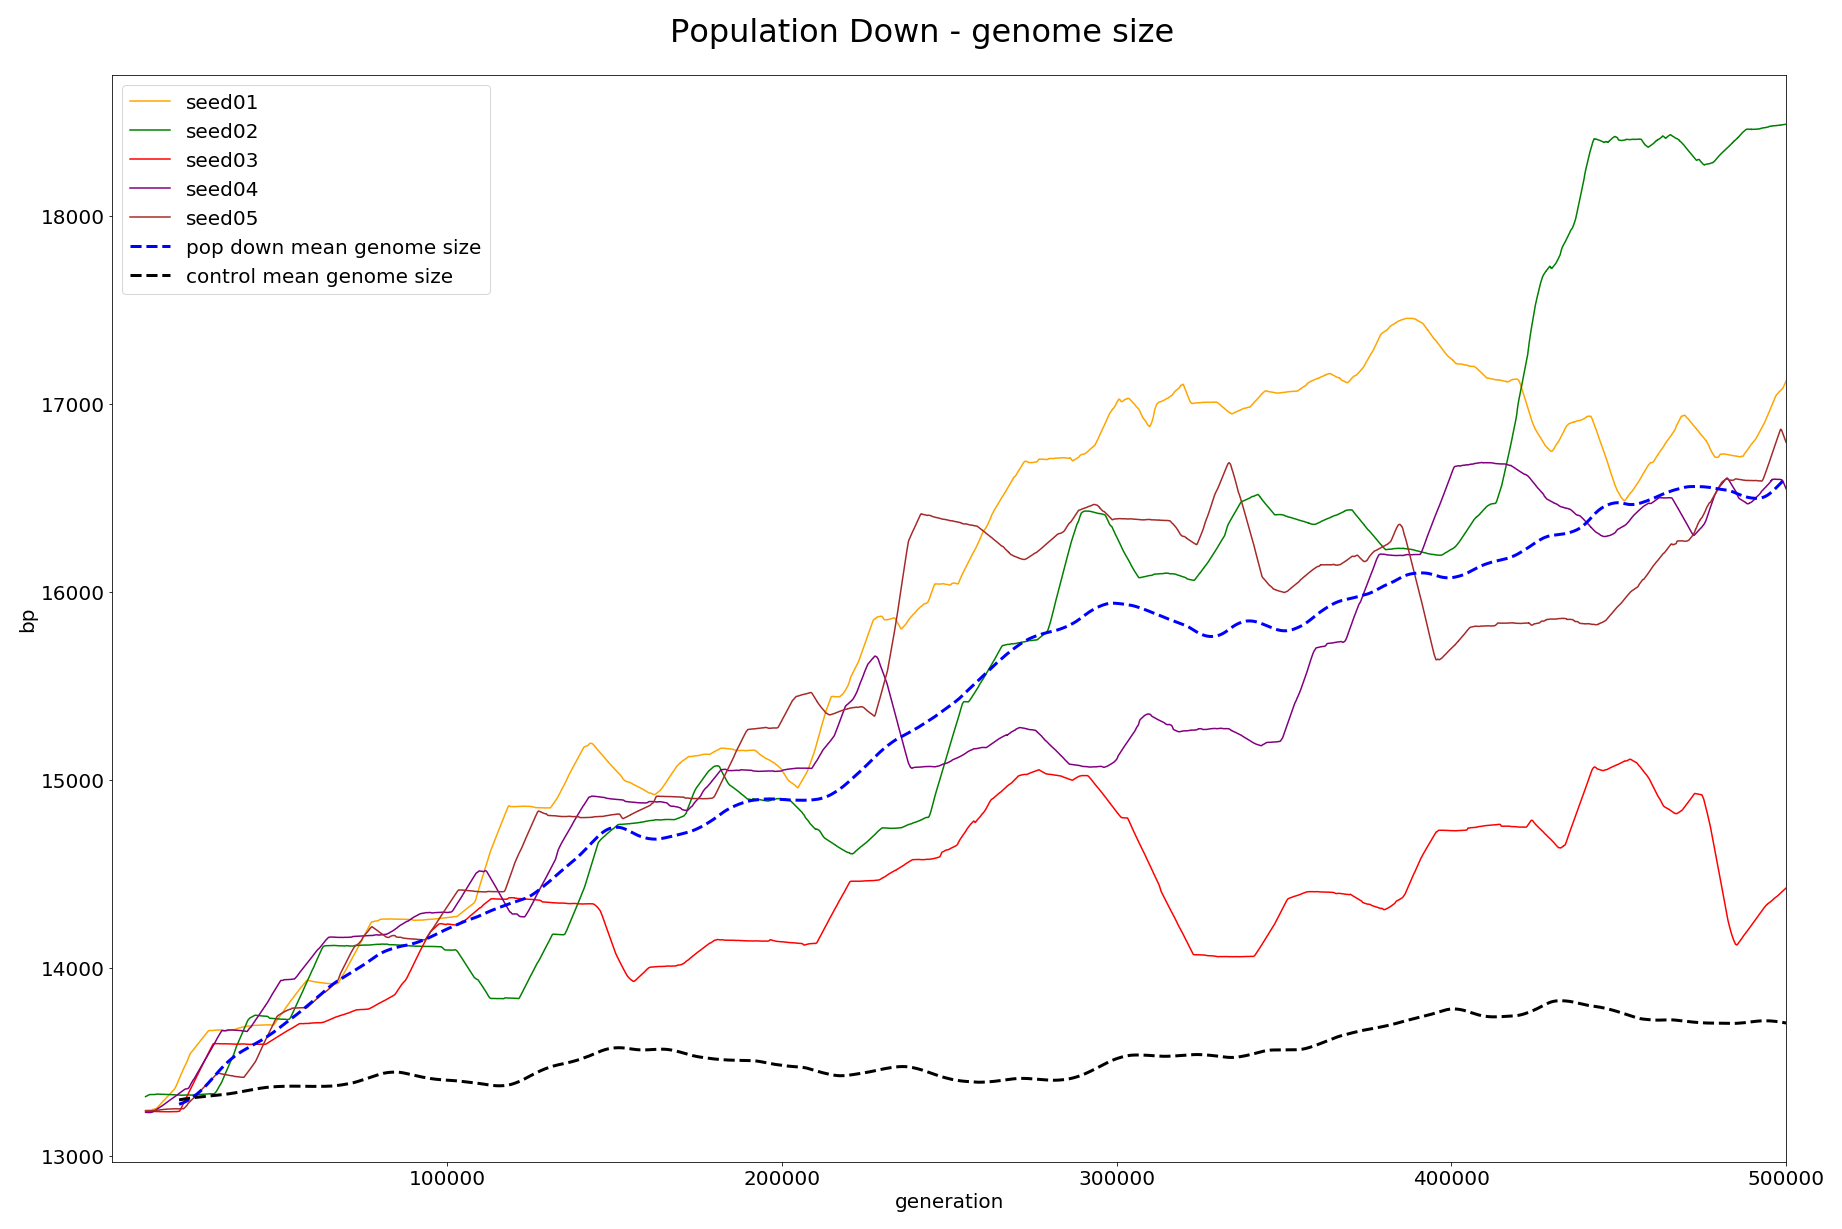
\includegraphics[width=\linewidth]{population_down_genome_size_b1-e500000}
	\caption[Population down genome size]{$N_-$ genome size, generations 1-500,000.}
	\label{fig:pop_down_genome_size}
\end{figure}

The $N_-$ condition ending up with a genome over 20\% larger than the control condition perfectly illustrates the effects of genetic drift described by Batut et al. with regard to small effective population sizes ($N_e$) \cite{Batut.2014}. The efficacy of selection to remove deleterious mutations and accumulations of non-coding bases is predicted to go down in populations with a smaller effective population size, causing rapid expansion of the genome size. This appears to be exactly what happened here, as Figure~\ref{fig:pop_down_perc_non-coding} shows the amount of non-coding bases greatly expanding, reaching 17.7\% over the control condition. 

\begin{figure}[H]
	\centering
	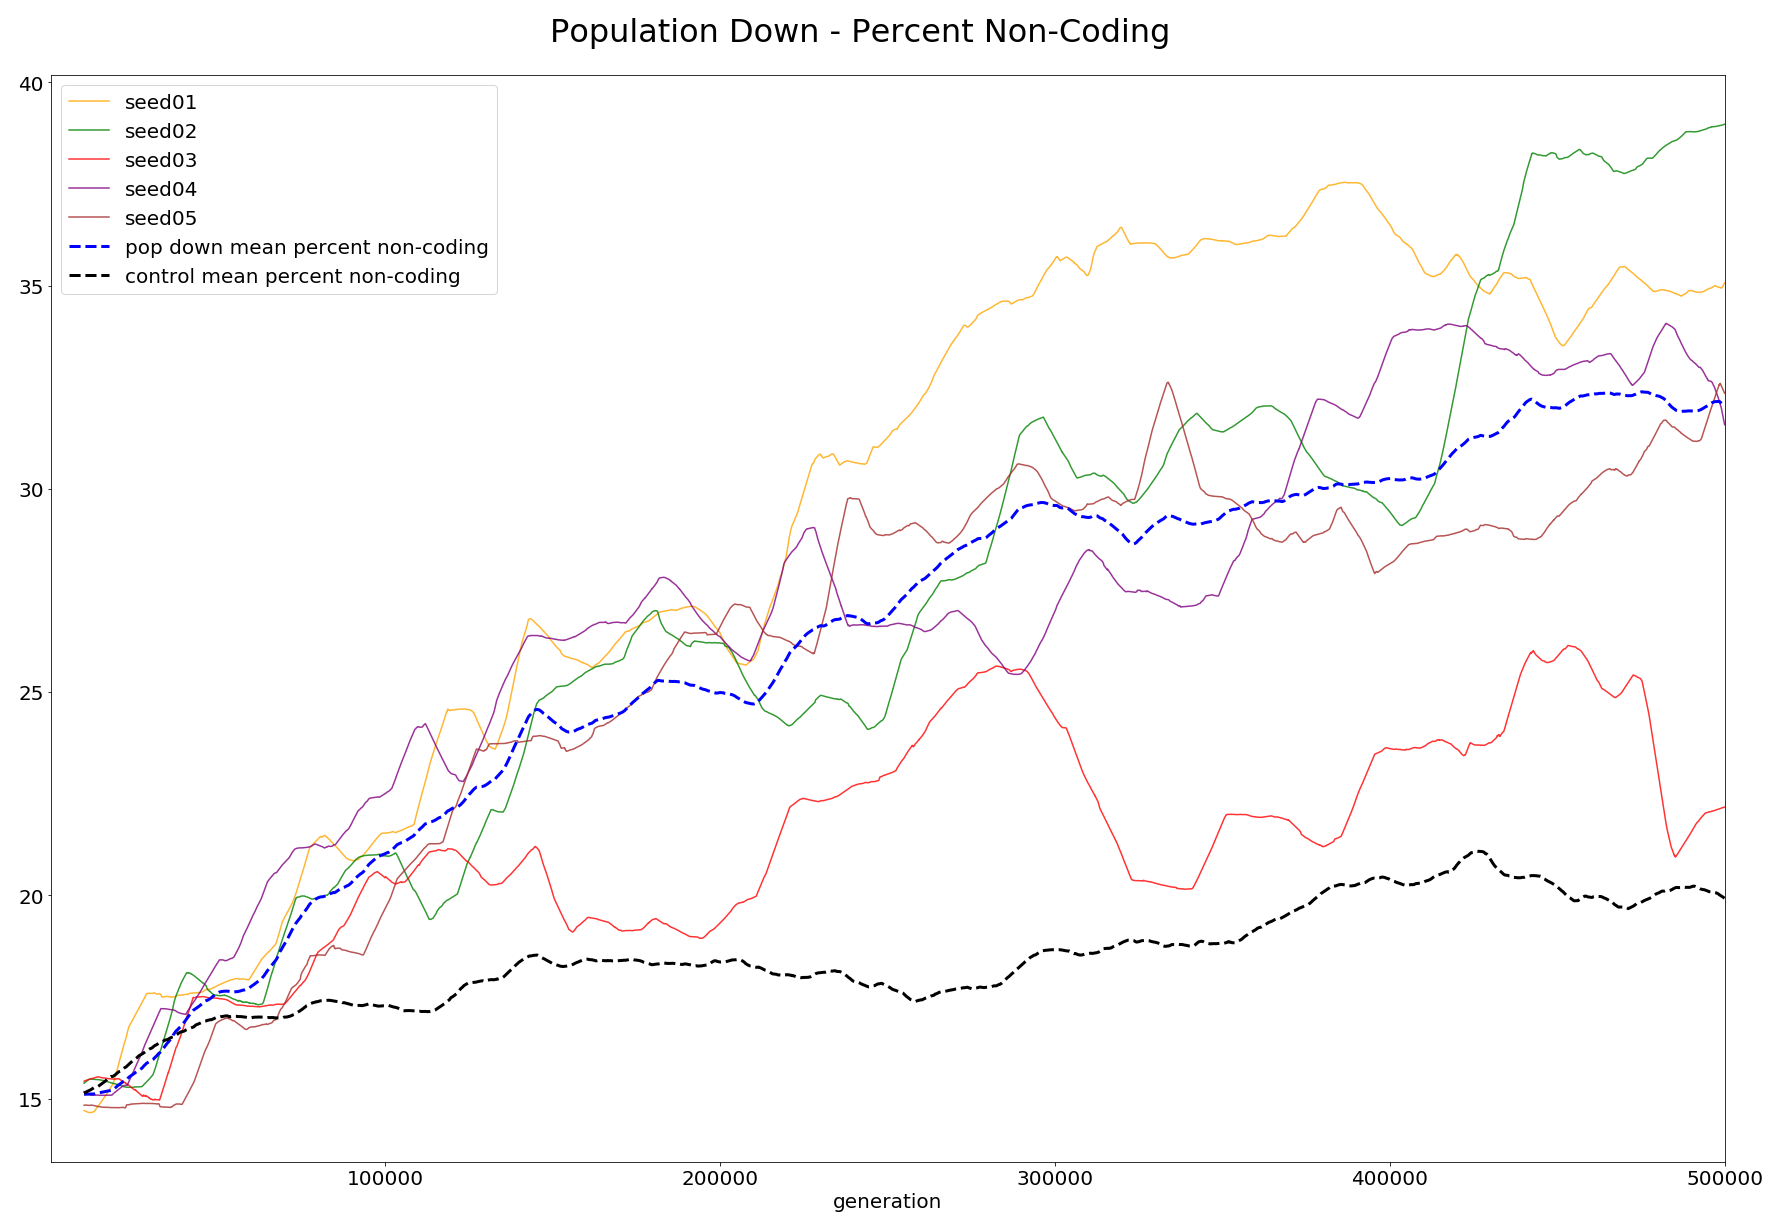
\includegraphics[width=\linewidth]{population_down_percent_non-coding_b1-e500000}
	\caption[Population down percent non-coding]{$N_-$ population mean percent non-coding, generations 1-500,000, all seeds.}
	\label{fig:pop_down_perc_non-coding}
\end{figure}

\subsection{Statistics}
In this section, statistics are given for the above conditions and the results are combined into single tables and graphs for ease of comparison. As above, the result are, unless specified otherwise, the mean across all seeds for all 500,000 generations.
\subsubsection{Genome Size}\label{sec:genome_size}

Figure~\ref{fig:genome_size} presents the main findings regarding genome size for all conditions. In the figure, the blue line shows the control condition and the other colors show the changed conditions: $\mu_+$/$\mu_-$ (mutation up/down), $k_+$/$k_-$ (selection up/down), and $N_+$/$N_-$ (population up/down). As can be seen from the figure, the expectations from Section~\ref{sec:expected_results} did not always hold up, as several conditions actually \textit{increased} over their original size. 
\begin{figure}[H]
	\centering
	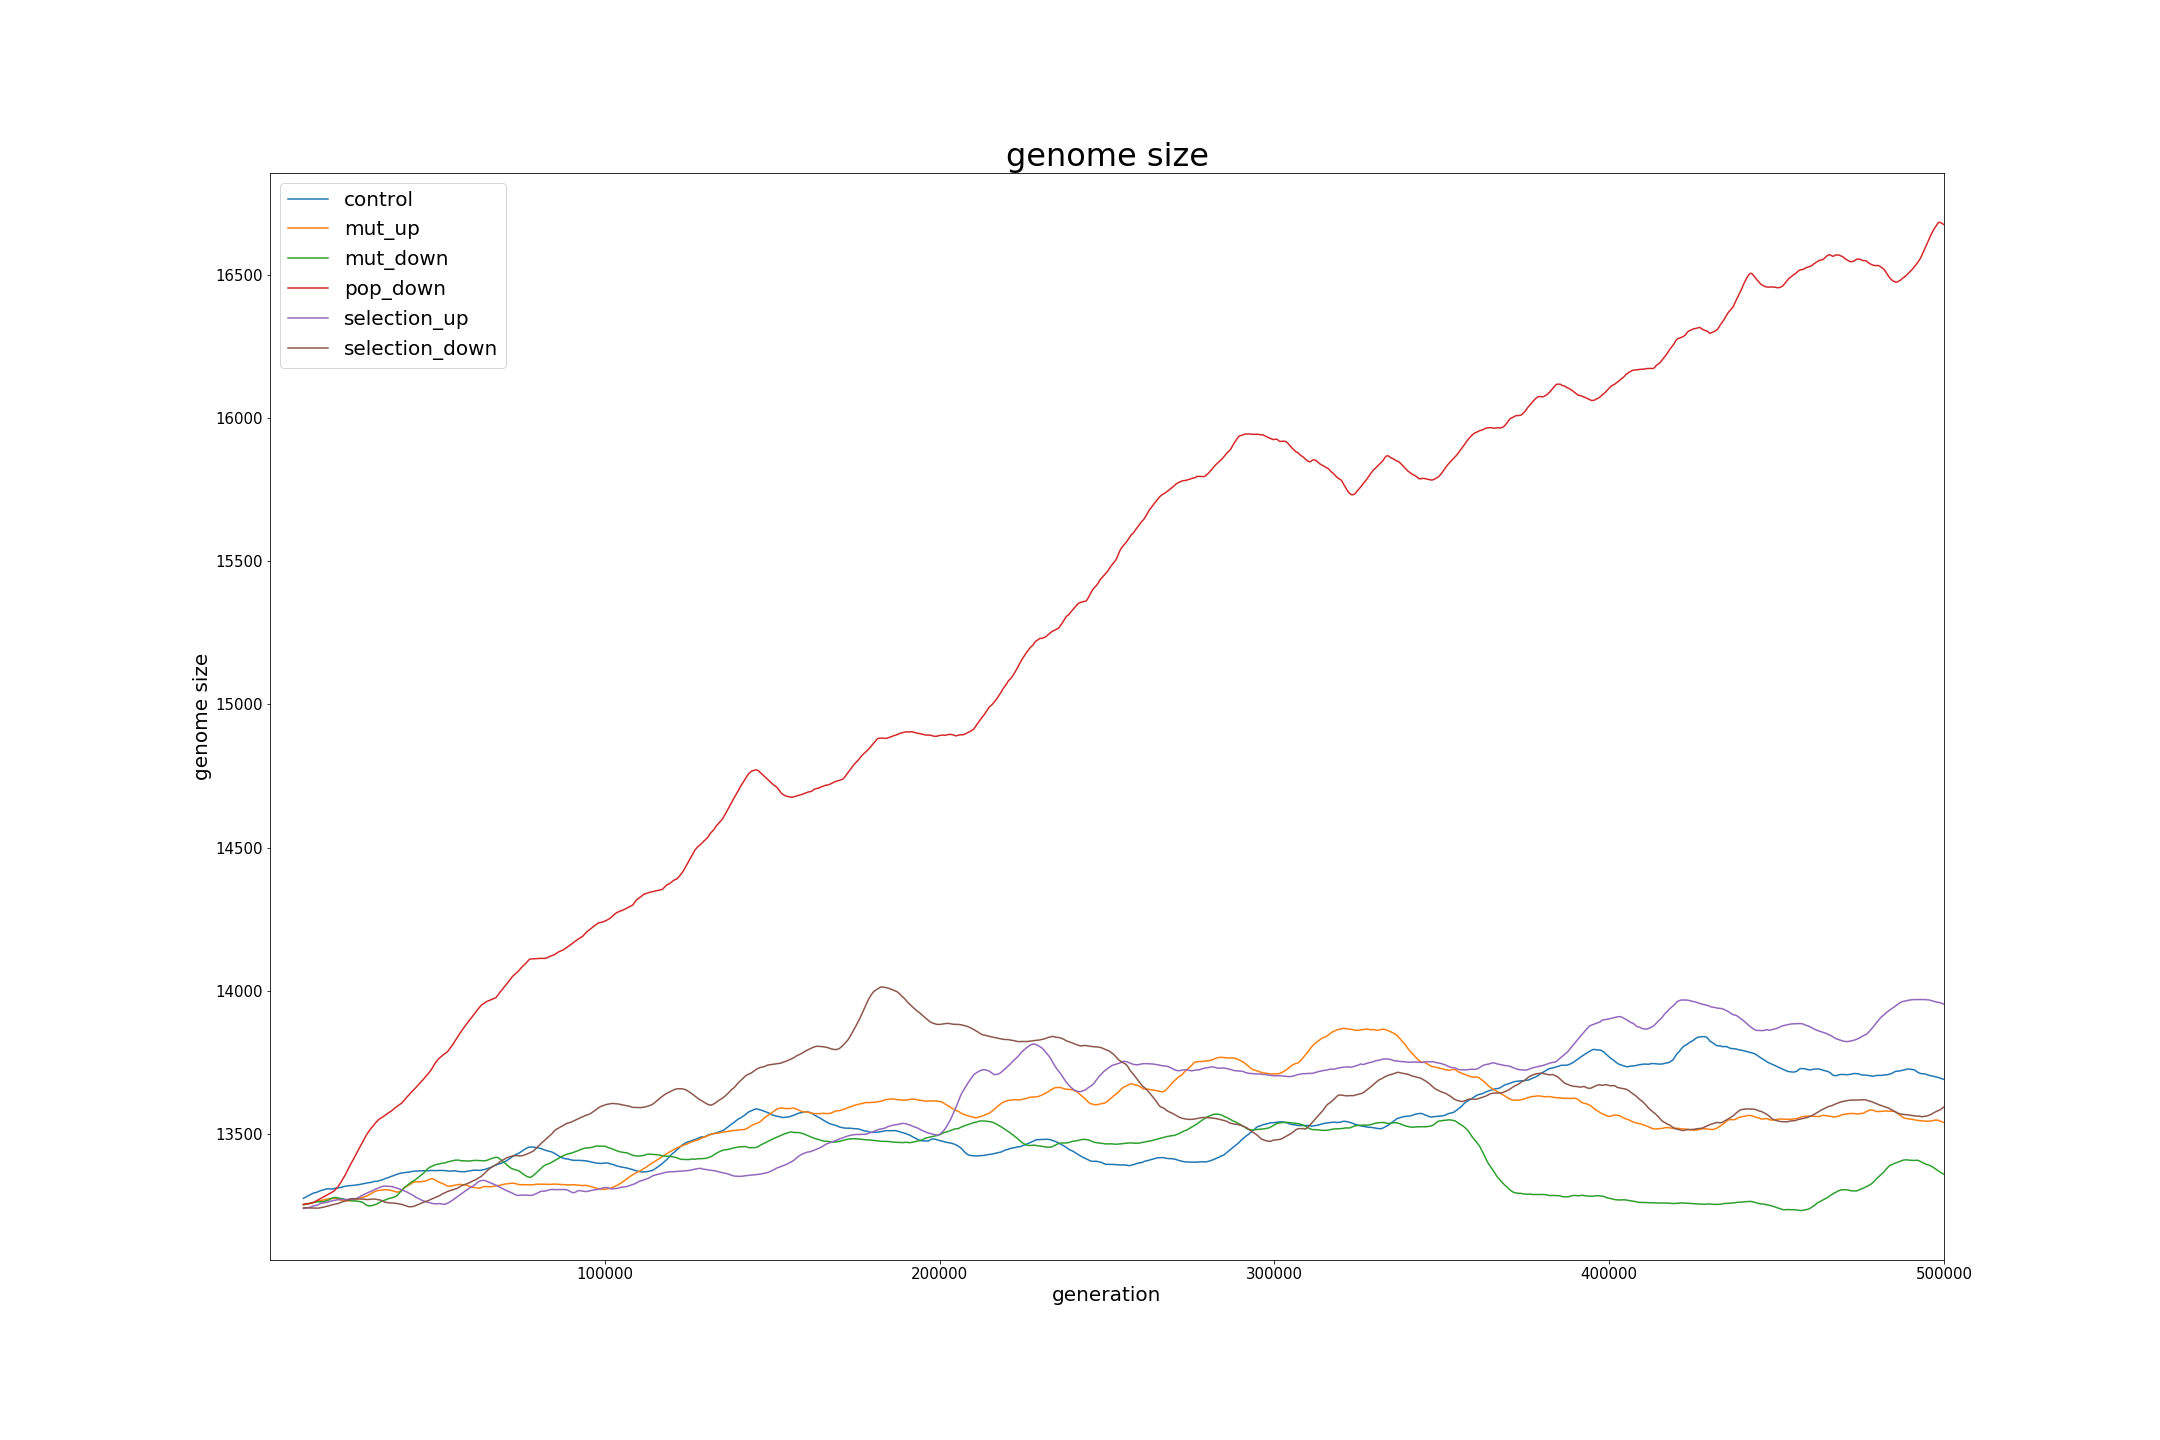
\includegraphics[width=\linewidth]{stat_fitness_global_mean_genome_size}
	\caption[Genome size]{Average genome size across the population, in number of bases, of all conditions. Average taken across all five seeds for each condition.}
	\label{fig:genome_size}
\end{figure}
In fact, the $N_-$ condition had a runaway increase in the number of bases, reaching over 16,500 bases at one time, a 25\% increase over the original wild type's roughly 13,200 bp. Even after 500,000 generations, it seems that the upper size limit may still not have been reached. The statistical results are given below in Tables~\ref{table:genome_size_stats} and \ref{table:genome_size_mean_and_std_dev}, which show the mean and standard deviation for all seeds across all 500,000 generations. 

\begin{table}[h]
	\begin{tabular}{|c|c|c|c|}
		\hline
		\multicolumn{4}{c}{\Large \textbf{Genome Size - 500k Gen. Mean \& Std. Dev. (in bp)}} \\
		\hline
		 & \textbf{mean} & \textbf{standard deviation} & \textbf{mean's \% change from control} \\
		 \hline
		 control & 13537.031513 & 144.351 & \textemdash \\ 
		 \hline
		 $\mu_+$ & 13558.374160 & 155.077847 & 0.157661 \\ 
		 \hline
		 $\mu_-$ & 13410.743690 & 101.376104 & -0.932906 \\ 
		 \hline
		 $k_+$ & 13621.901104 & 229.635708 & 0.626944 \\ 
		 \hline
		 $k_-$ & 13614.663599 & 172.675042 & 0.573479 \\ 
		 \hline
		 $N_+$ & 13119.243838 & 230.240517 & -3.086258 \\ 
		 \hline
		 $N_-$ & 15275.149392 & 950.266243 & 12.839727 \\ 
		 \hline
	\end{tabular}
	\caption[Genome size - mean and std. dev.]{Average genome size across all 500,000 generations, with standard deviation for all seeds and all conditions. }
	\label{table:genome_size_mean_and_std_dev}
\end{table}

\begin{table}[h]
	\centering
	\begin{tabular}{|c|c|c|}
		\hline
		\multicolumn{3}{c}{\Large Genome Size - Rank Sum \& P-Values} \\
		\hline
		& \textbf{rank sum U} & \textbf{p-value} \\
		\hline\hline
		$\mu_+$ & 110508011469.50 & 0.00000000 \\ 
		\hline
		$\mu_-$ & 71008638349.50 & 0.00000000 \\ 
		\hline
		$k_+$ & 100151680984.50 & 0.00000000 \\ 
		\hline
		$k_-$ & 88533681875.00 & 0.00000000 \\ 
		\hline
		$N_+$ & 21845365773.50 & 0.00000000 \\ 
		\hline
		$N_-$ & 16477791900.50 & 0.00000000 \\ 
		\hline
	\end{tabular}
	\caption[Genome size rank sum statistics]{Genome size rank sum statistics.}
	\label{table:genome_size_stats}
\end{table} 

Of the remaining conditions, all but the $k_+$ condition (which had an an increase of 11\% over the control condition) ended up with fewer base pairs than the control condition, though all increased slightly over their starting point. Also noteworthy is that the mutation down condition appears to have had a steady increase in the number of base pairs until a maximum of just over 14,000 around generation 350,000 before having a fairly sharp decline back to nearly the original size. 

Examining the percent changed from the control condition shown in Figure~\ref{fig:genome_size_percent_change} it can be seen that at points, the $\mu_-$ condition was nearly 5\% smaller than the control condition. 

\begin{figure}[H]
	\centering
	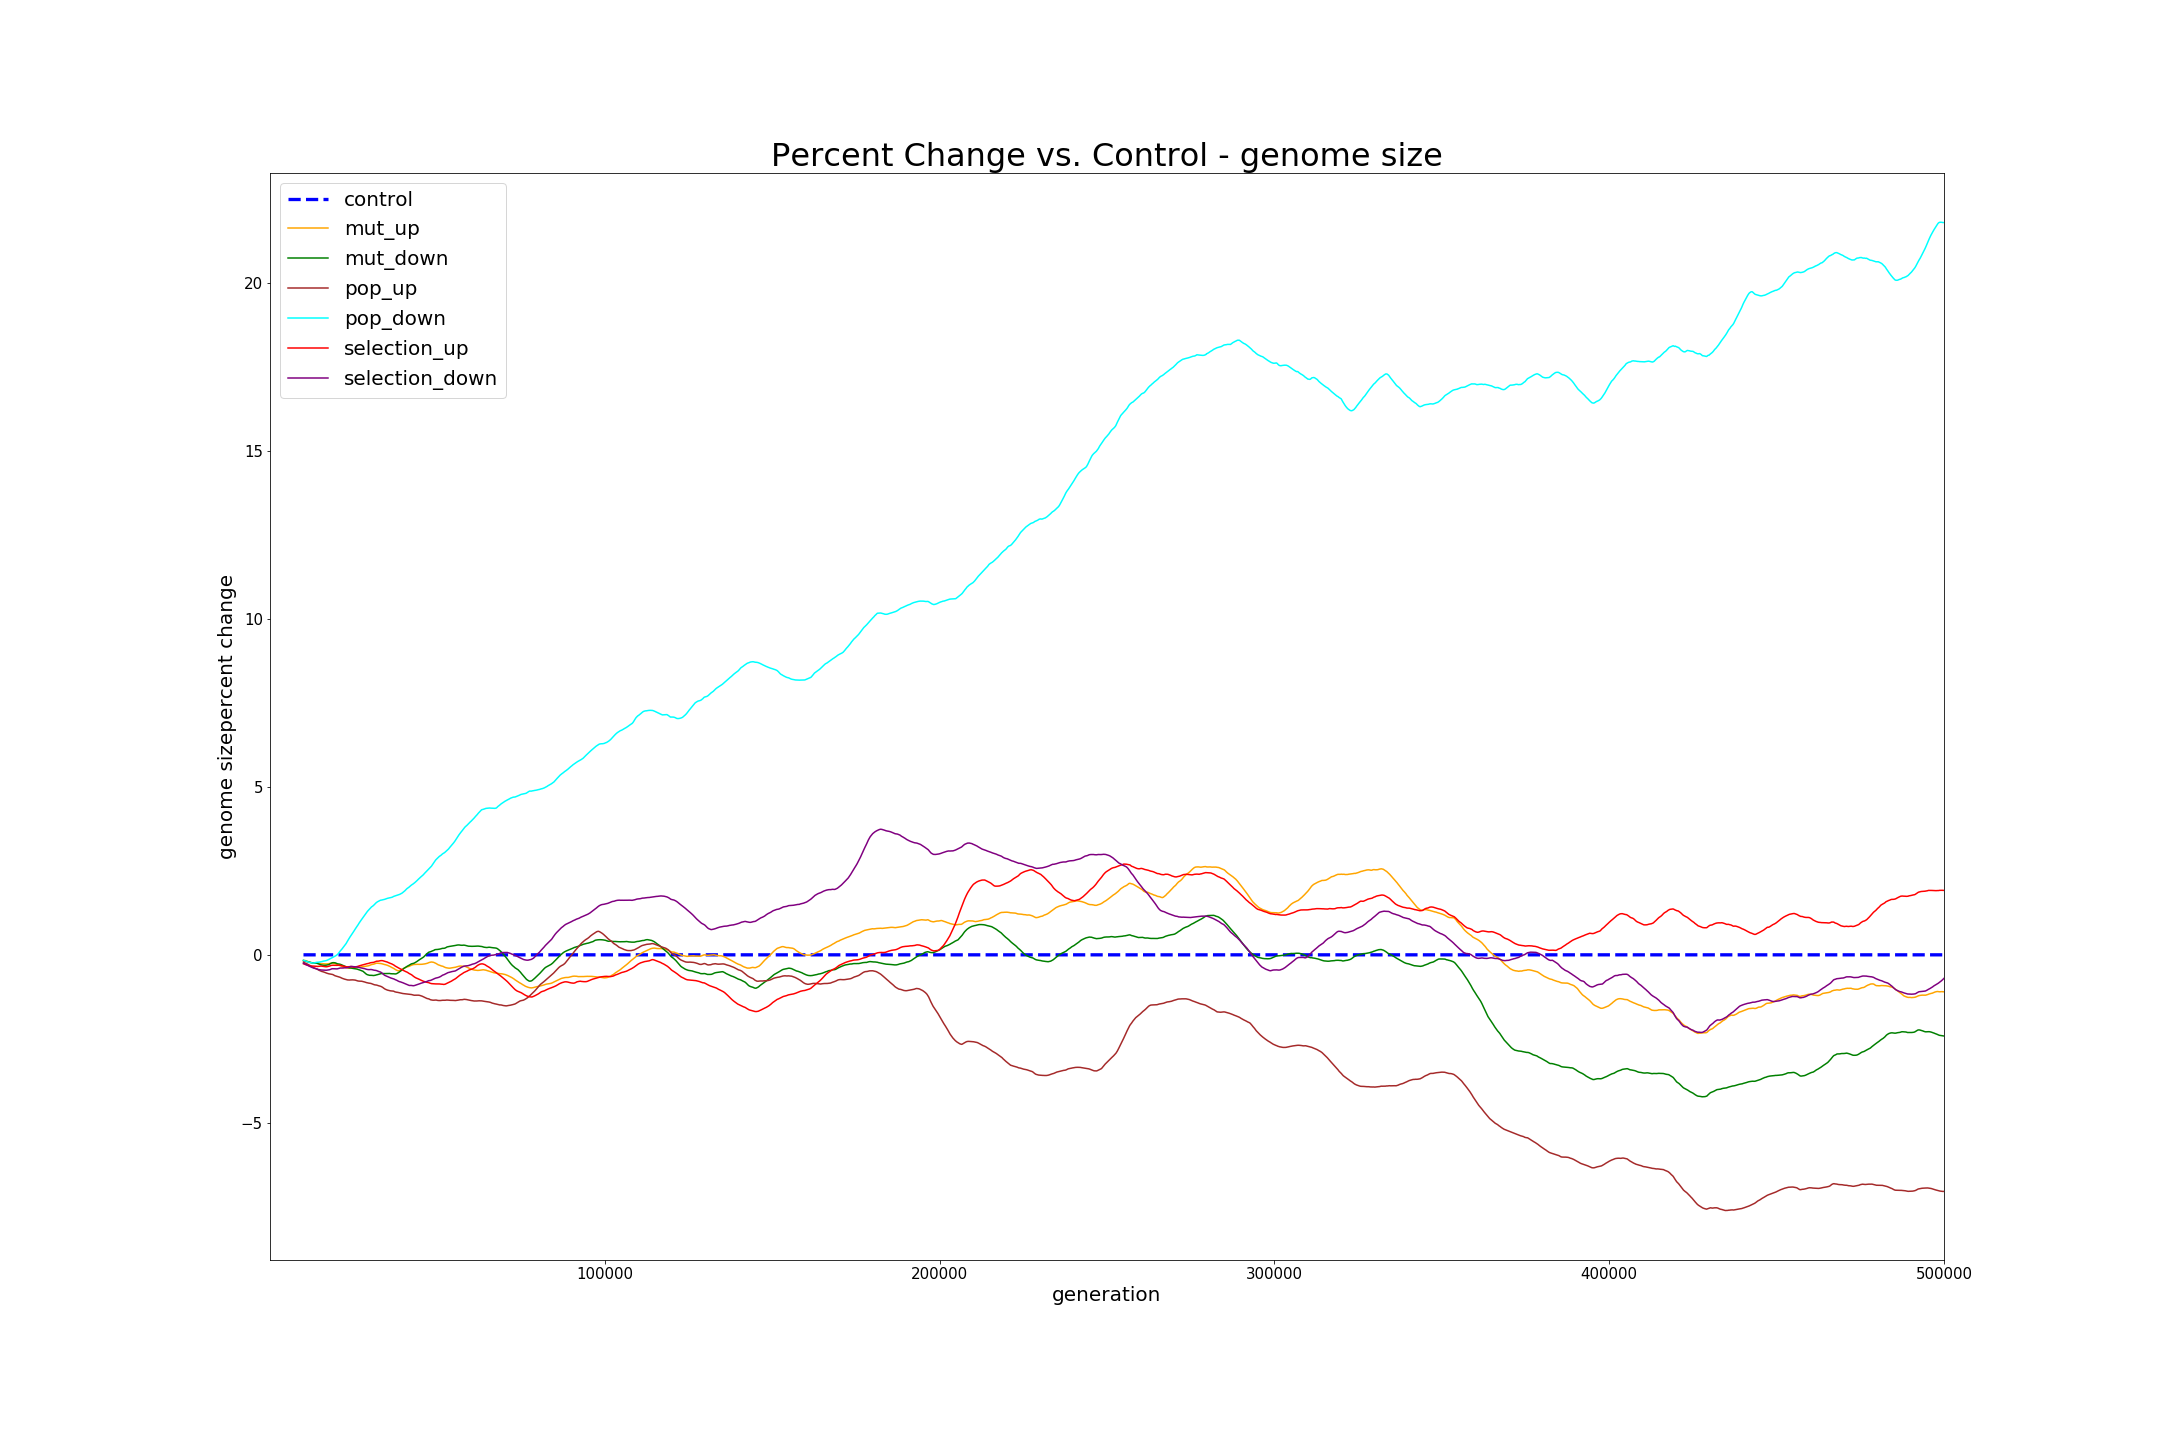
\includegraphics[width=\linewidth]{stat_fitness_perc_change_genome_size}
	\caption[Genome size - percent change]{Genome size's percent change from the control condition.}
	\label{fig:genome_size_percent_change}
\end{figure}

Lastly, a zoomed-in look at just the last 50,000 generations is provided in Figure~\ref{fig:genome_size_last_50k}, allowing a clearer distinction between the control and other conditions. The respective statistics are given in Table~\ref{table:genome_size_stats_last_50k}. In the figure, the horizontal dashed black line gives the control condition's genome size at generation 0, the blue dashed line gives the mean genome size across all control seeds, and the colored dashed lines in each figure give the mean of the seeds for that condition. 
\begin{figure}[H]
	\centering
	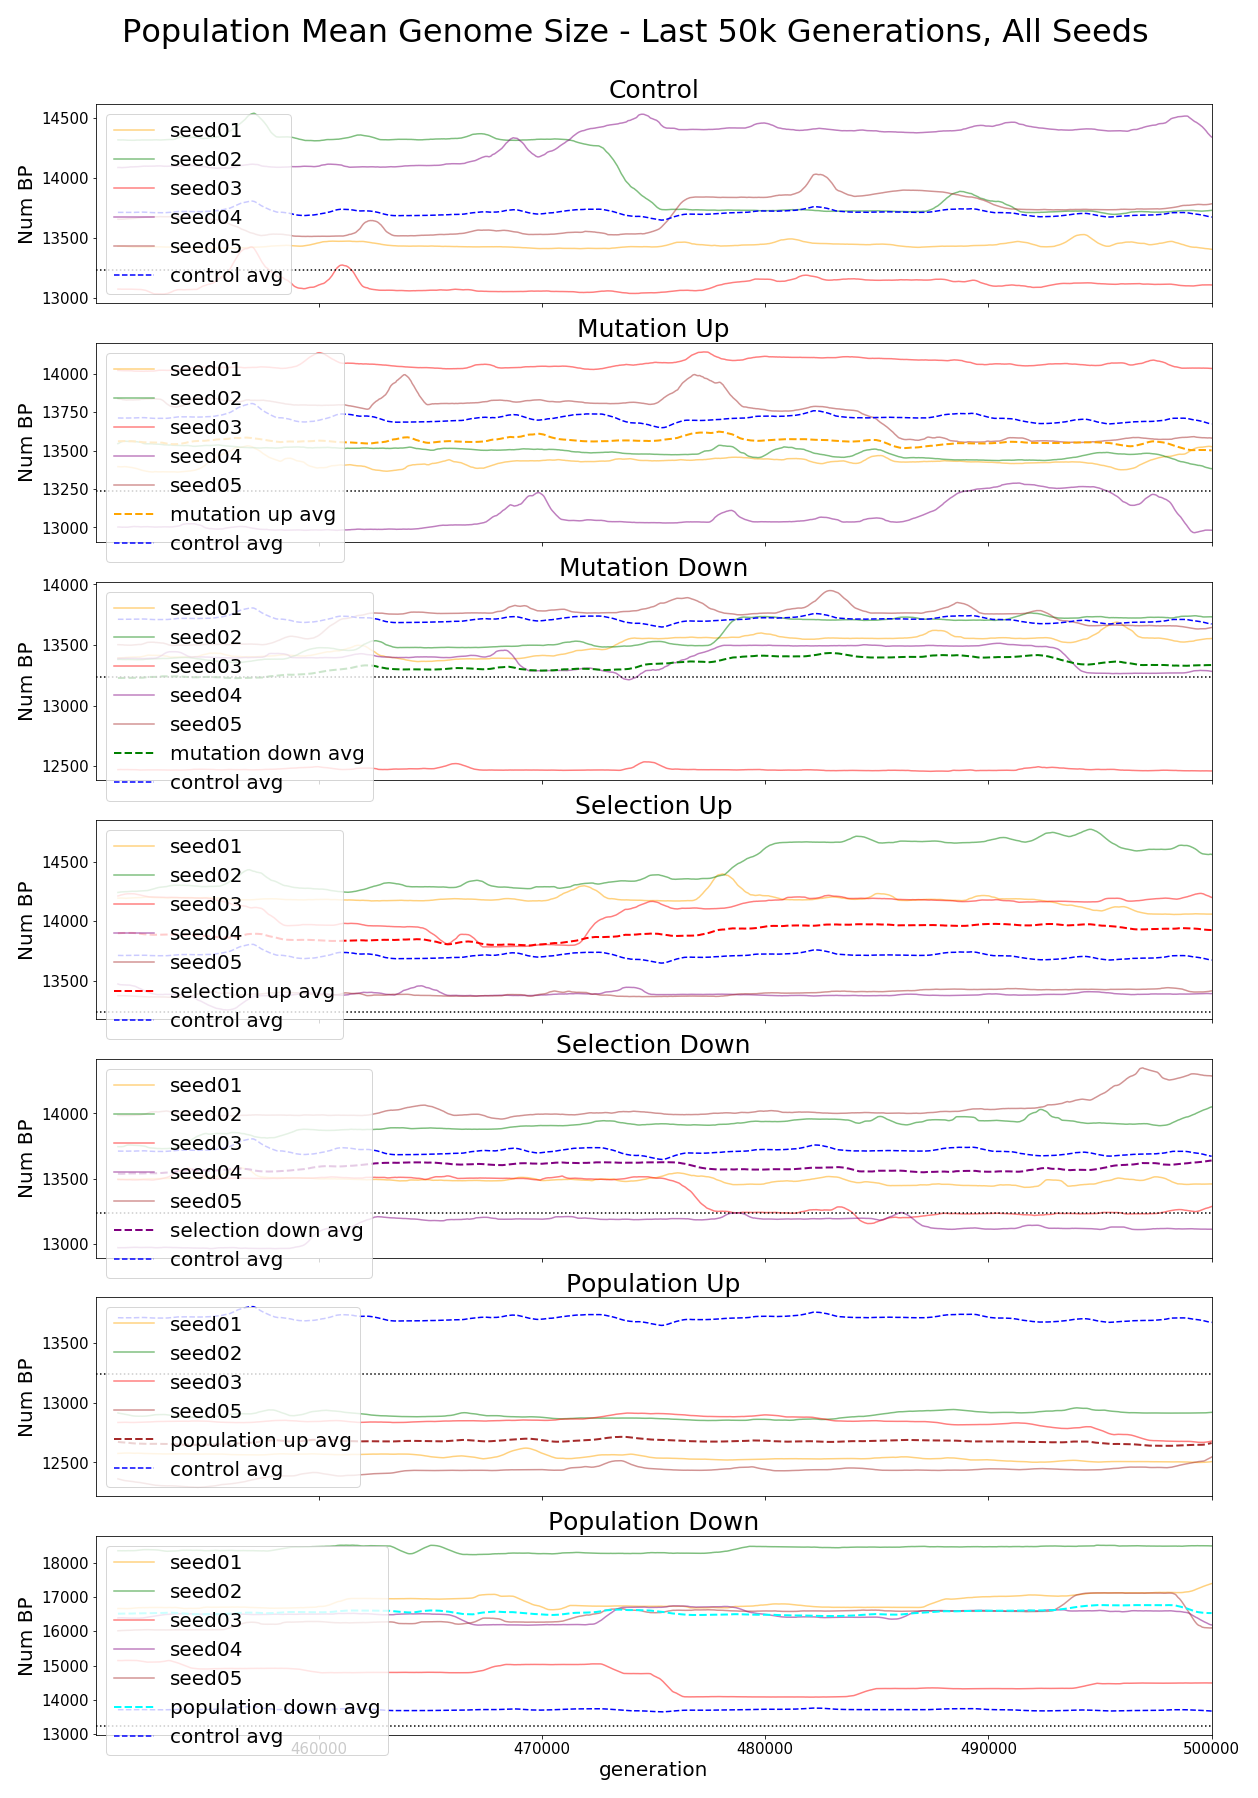
\includegraphics[width=\linewidth]{genome_size_last_50k_all_seeds}
	\caption[Genome size - last 50k generations]{Genome Size - Last 50k Generations, all seeds, all conditions. All seeds are shown (colored, solid lines) as well as the mean across all seeds for each condition (colored, dashed lines) are given. The black dashed line is the genome size at generation 0 in the control condition.}
	\label{fig:genome_size_last_50k}
\end{figure}

\begin{table}[H]
	\begin{tabular}{|c|c|c|c|}
		\hline
		\multicolumn{4}{c}{\textbf{Genome Size - Last 50k Gen. Mean \& Std. Dev.}} \\
		\hline
		& \textbf{Mean} & \textbf{Std. Dev} & \textbf{\% change from control} \\
		\hline
		control & 13710.785821 & 23.9975 & \textemdash \\ 
		\hline
		$\mu_+$ & 13560.671469 & 21.360848 & -1.094863 \\ 
		\hline
		$\mu_-$ & 13332.739494 & 61.121661 & -2.757291 \\ 
		\hline
		$k_+$ & 13901.869266 & 57.819805 & 1.393672 \\ 
		\hline
		$k_-$ & 13587.959325 & 27.504289 & -0.895838 \\ 
		\hline
		$N_+$ & 12680.917724 & 12.583662 & -7.511372 \\ 
		\hline
		$N_-$ & 16562.744322 & 80.705805 & 20.800839 \\ 
		\hline
	\end{tabular}
	\caption[Genome size - last 50k generations mean \& std. dev.]{This table shows the mean, standard deviation, and percent change from the control condition for the population for just the last 50k generations.}
	\label{table:genome_size_stats_last_50k}
\end{table}


\subsubsection{Metabolic Error and Fitness}\label{res:metabolic_error_and_fitness}
Figure~\ref{fig:mean_fitness_all_seeds} shows three categories of information for each condition: 1) the mean population fitness for each seed (in various colors), 2) the mean fitness across all seeds for that condition (dashed line, black), and 3) the control condition (dashed line, blue) for each condition.   

\begin{figure}[H]
	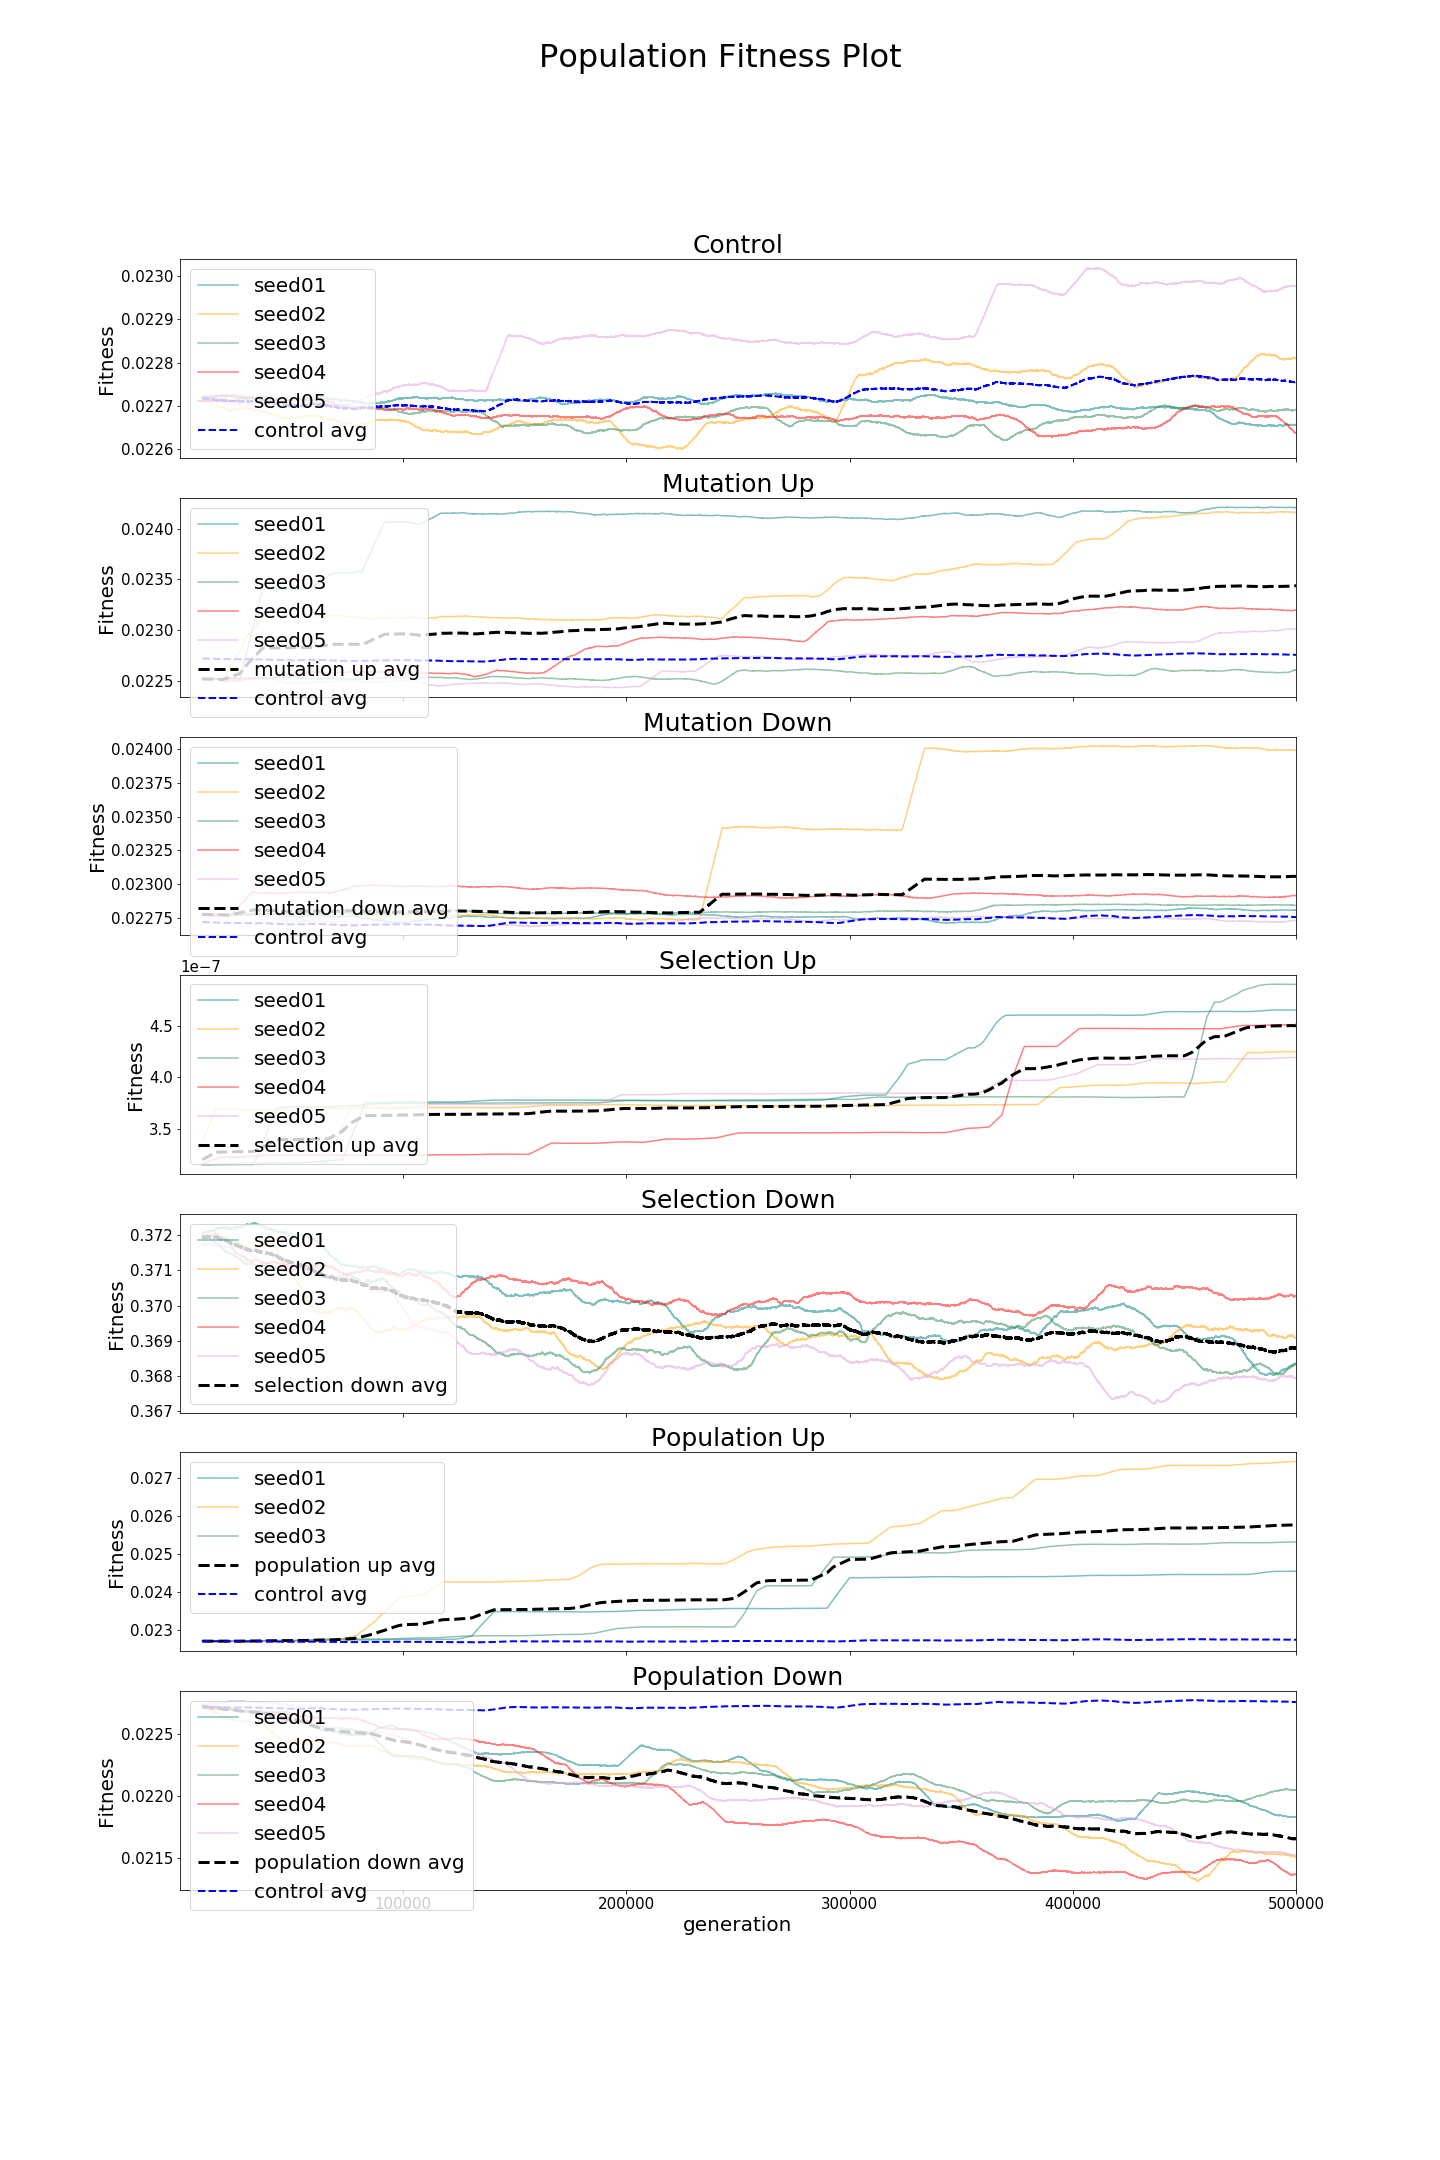
\includegraphics[width=\linewidth]{global_fitness_all_seeds}
	\caption[Fitness all seeds all conditions]{Mean population fitness for each condition. All seeds are shown; the average for that condition is shown in black and the control condition is blue.}
	\label{fig:mean_fitness_all_seeds}
\end{figure}

\begin{figure}[H]
	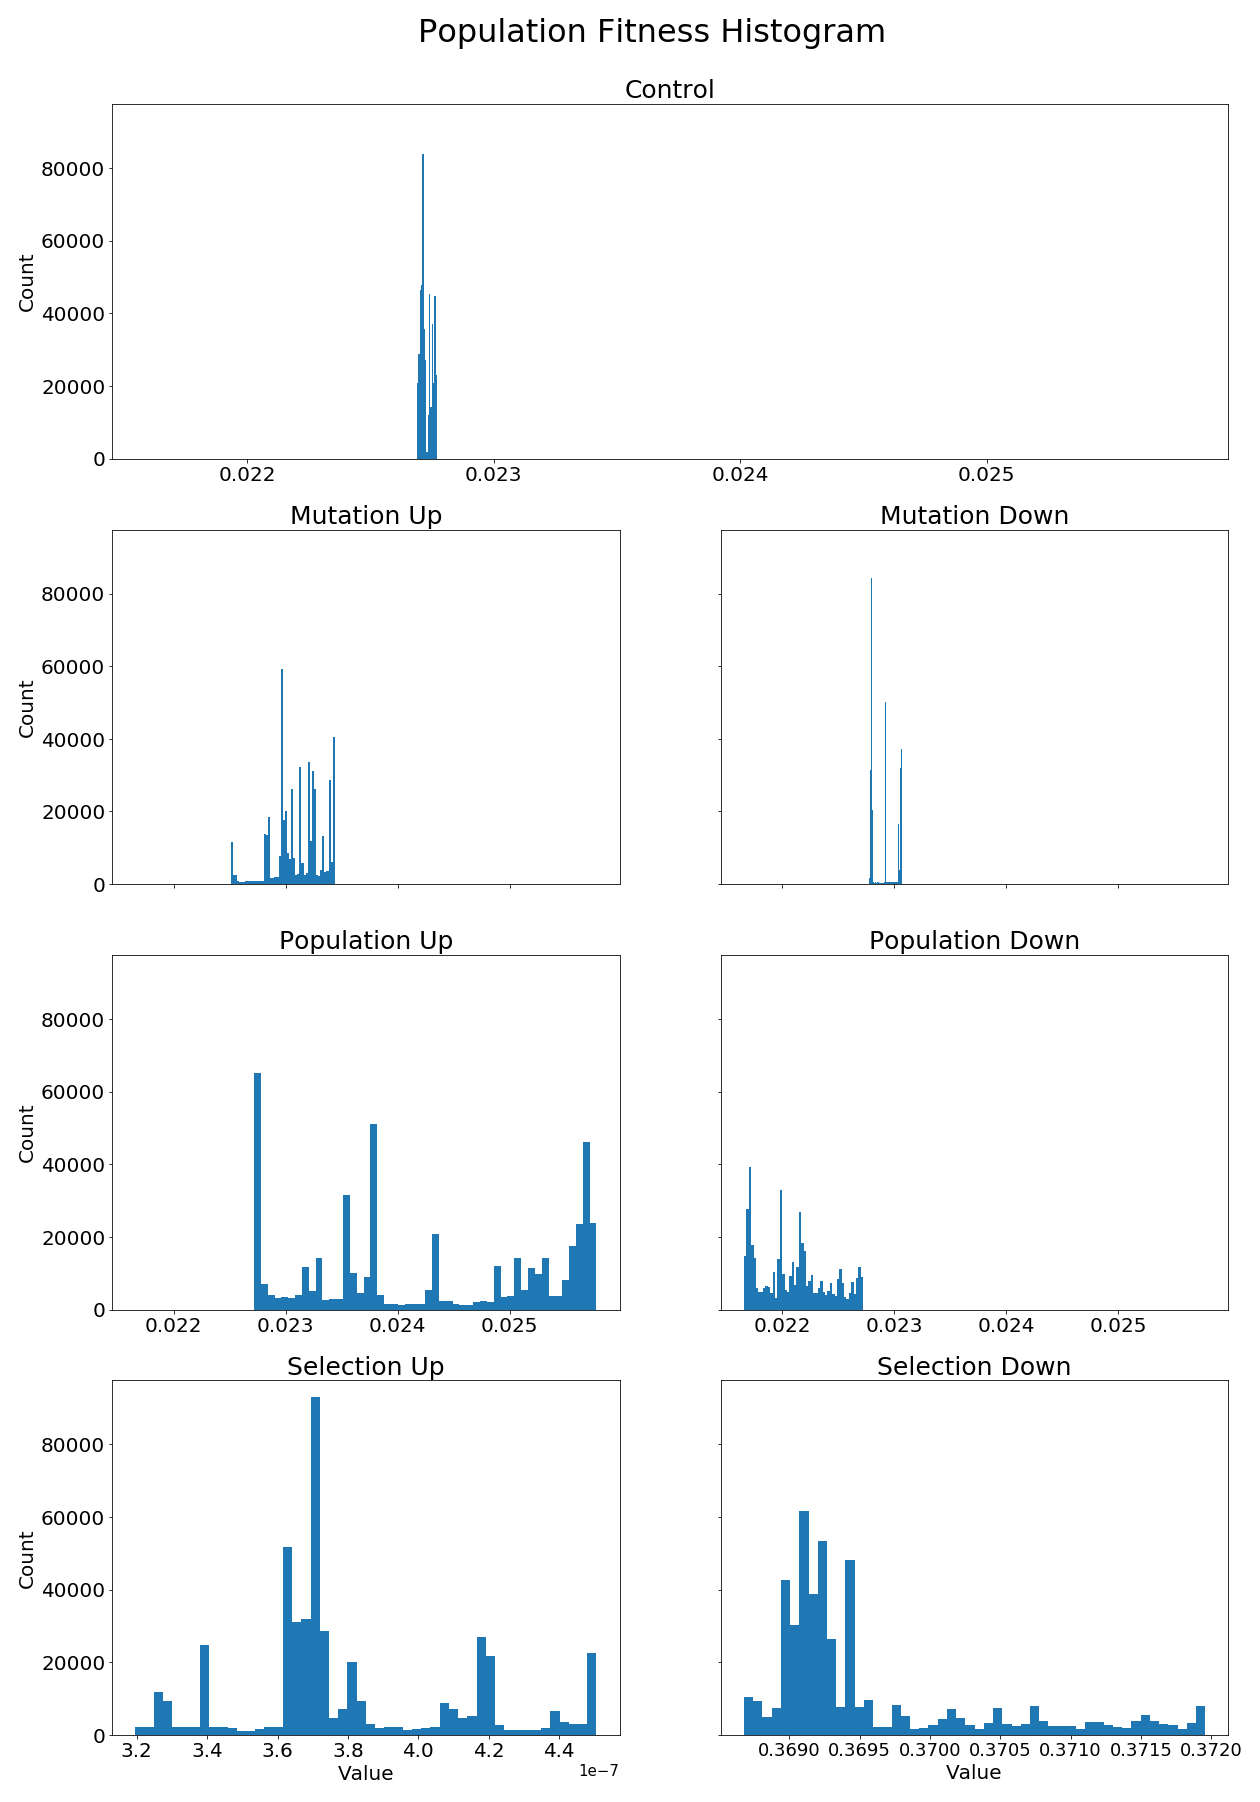
\includegraphics[width=\linewidth]{population_mean_fitness_histogram}
	\caption[Mean fitness histogram]{Histogram of population fitness at generation 500,000 for all conditions. Note that the x-axes for both the $k_+$ and $k_-$ conditions are on a different scale relative to the other conditions and each other.}
	\label{fig:global_fitness_histogram}
\end{figure}
Figure~\ref{fig:global_fitness_histogram} shows a histogram of the population mean fitness values for all conditions over the 500k generations. This figure is included to show the relative "stability" of a condition, i.e. to show how many times the fitness changed throughout the simulations. For example, although the $\mu_-$ condition ended the simulations in the most similar position to the control condition regarding fitness (just 0.8\% away), the more even distribution of the value counts for the control condition given in Figure~\ref{fig:global_fitness_histogram} makes it clear that the control condition experienced more fluctuations in value throughout the simulation. By contrast, the $\mu_-$ condition, as expected, tended to hover at certain locations in between rarer mutation events. This directly correlates to evolvability (see Section~\ref{res:evolvability}). 

Figure~\ref{fig:mean_metabolic_error} shows the mean metabolic error across all seeds for the whole population over time with respect to each condition. 
\begin{figure}[H]
	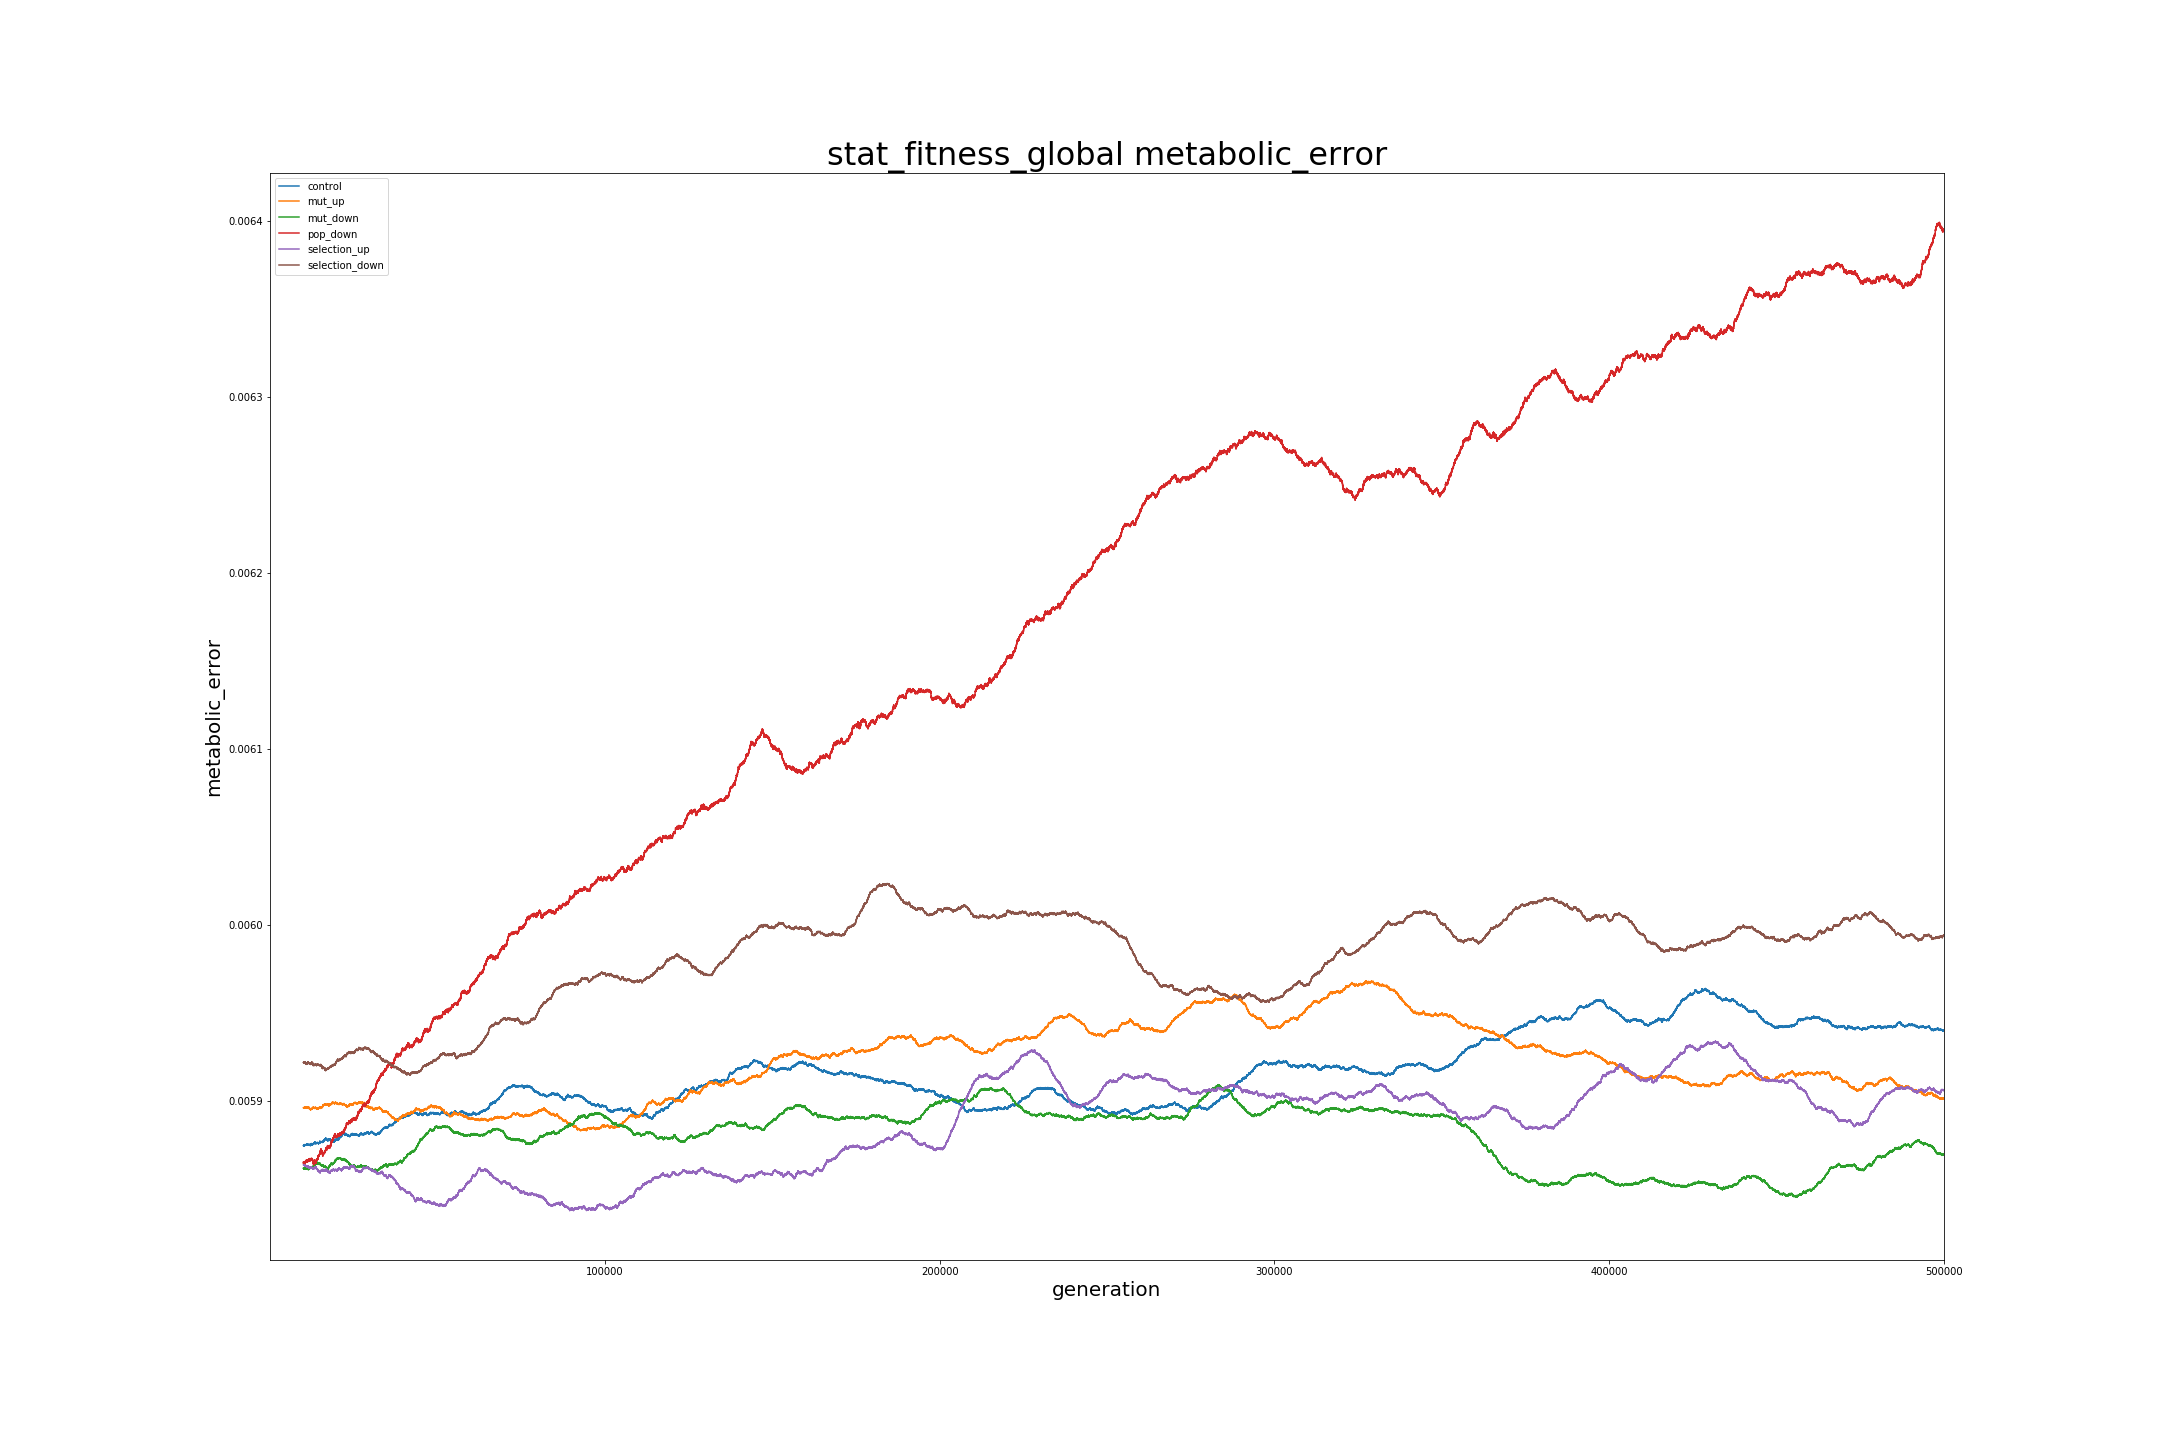
\includegraphics[width=\linewidth]{stat_fitness_global_mean_metabolic_error}
	\caption[Metabolic error]{Plot of the population mean metabolic error over time for all conditions, average of all seeds}
	\label{fig:mean_metabolic_error}
\end{figure}

Table~\ref{table:fitness_means_std_dev} below gives the mean fitness scores for the population and the differing conditions. 
\begin{table}[H]
	\centering
	\begin{tabular}{|c||c|c|c|}
		\hline
		\multicolumn{4}{c}{\Large \textbf{Fitness}} \\
		\hline
		& \textbf{mean} & \textbf{standard deviation} & \textbf{mean's \% change from control} \\
		\hline \hline
		control & 2.272542e-02 & 2.34433e-05 & \textemdash \\ 
		\hline
		$\mu_+$ & 2.310701e-02 & 2.191826e-04 & 1.679131 \\ 
		\hline
		$\mu_-$ & 2.290879e-02 & 1.180940e-04 & 0.806895 \\ 
		\hline
		$k_+$ & 3.803823e-07 & 3.130504e-08 & -99.998326 \\ 
		\hline
		$k_-$ & 3.695935e-01 & 8.101732e-04 & 1526.344327 \\ 
		\hline
		$N_+$ & 2.378802e-02 & 7.072942e-04 & 4.675849 \\ 
		\hline
		$N_-$ & 2.209722e-02 & 3.104264e-04 & -2.764272 \\ 
		\hline
	\end{tabular}
	\caption[Fitness means and standard deviations.]{Population mean fitness, standard deviations, and percent change from the control condition across all seeds. }
	\label{table:fitness_means_std_dev}
\end{table}

\subsection{Genome Structure}
In this section, the effects of the differing conditions on the structure of the genome as measured by the criteria in Tables~\ref{table:aevol_stats_genes_and_bp} and~\ref{table:aevol_stats_fitness_and_mutation} is examined. 

\subparagraph{Non-coding DNA}
One important factor in genome structure is the amount of non-coding DNA, i.e. the number of bases which are part of a genome but which do not encode protein sequences. Aevol gives the number of bases which are not in any coding sequence, as well as the total genome size, so one may easily calculate this percentage. The results from the experiments for all conditions are shown in Figure~\ref{fig:mean_non-coding_DNA}. Recalling genome size in Figure~\ref{fig:genome_size}, it seems that as the genome size of the population down condition rapidly expanded, most of those expansions were non-coding.
\begin{figure}[H]
	\centering
	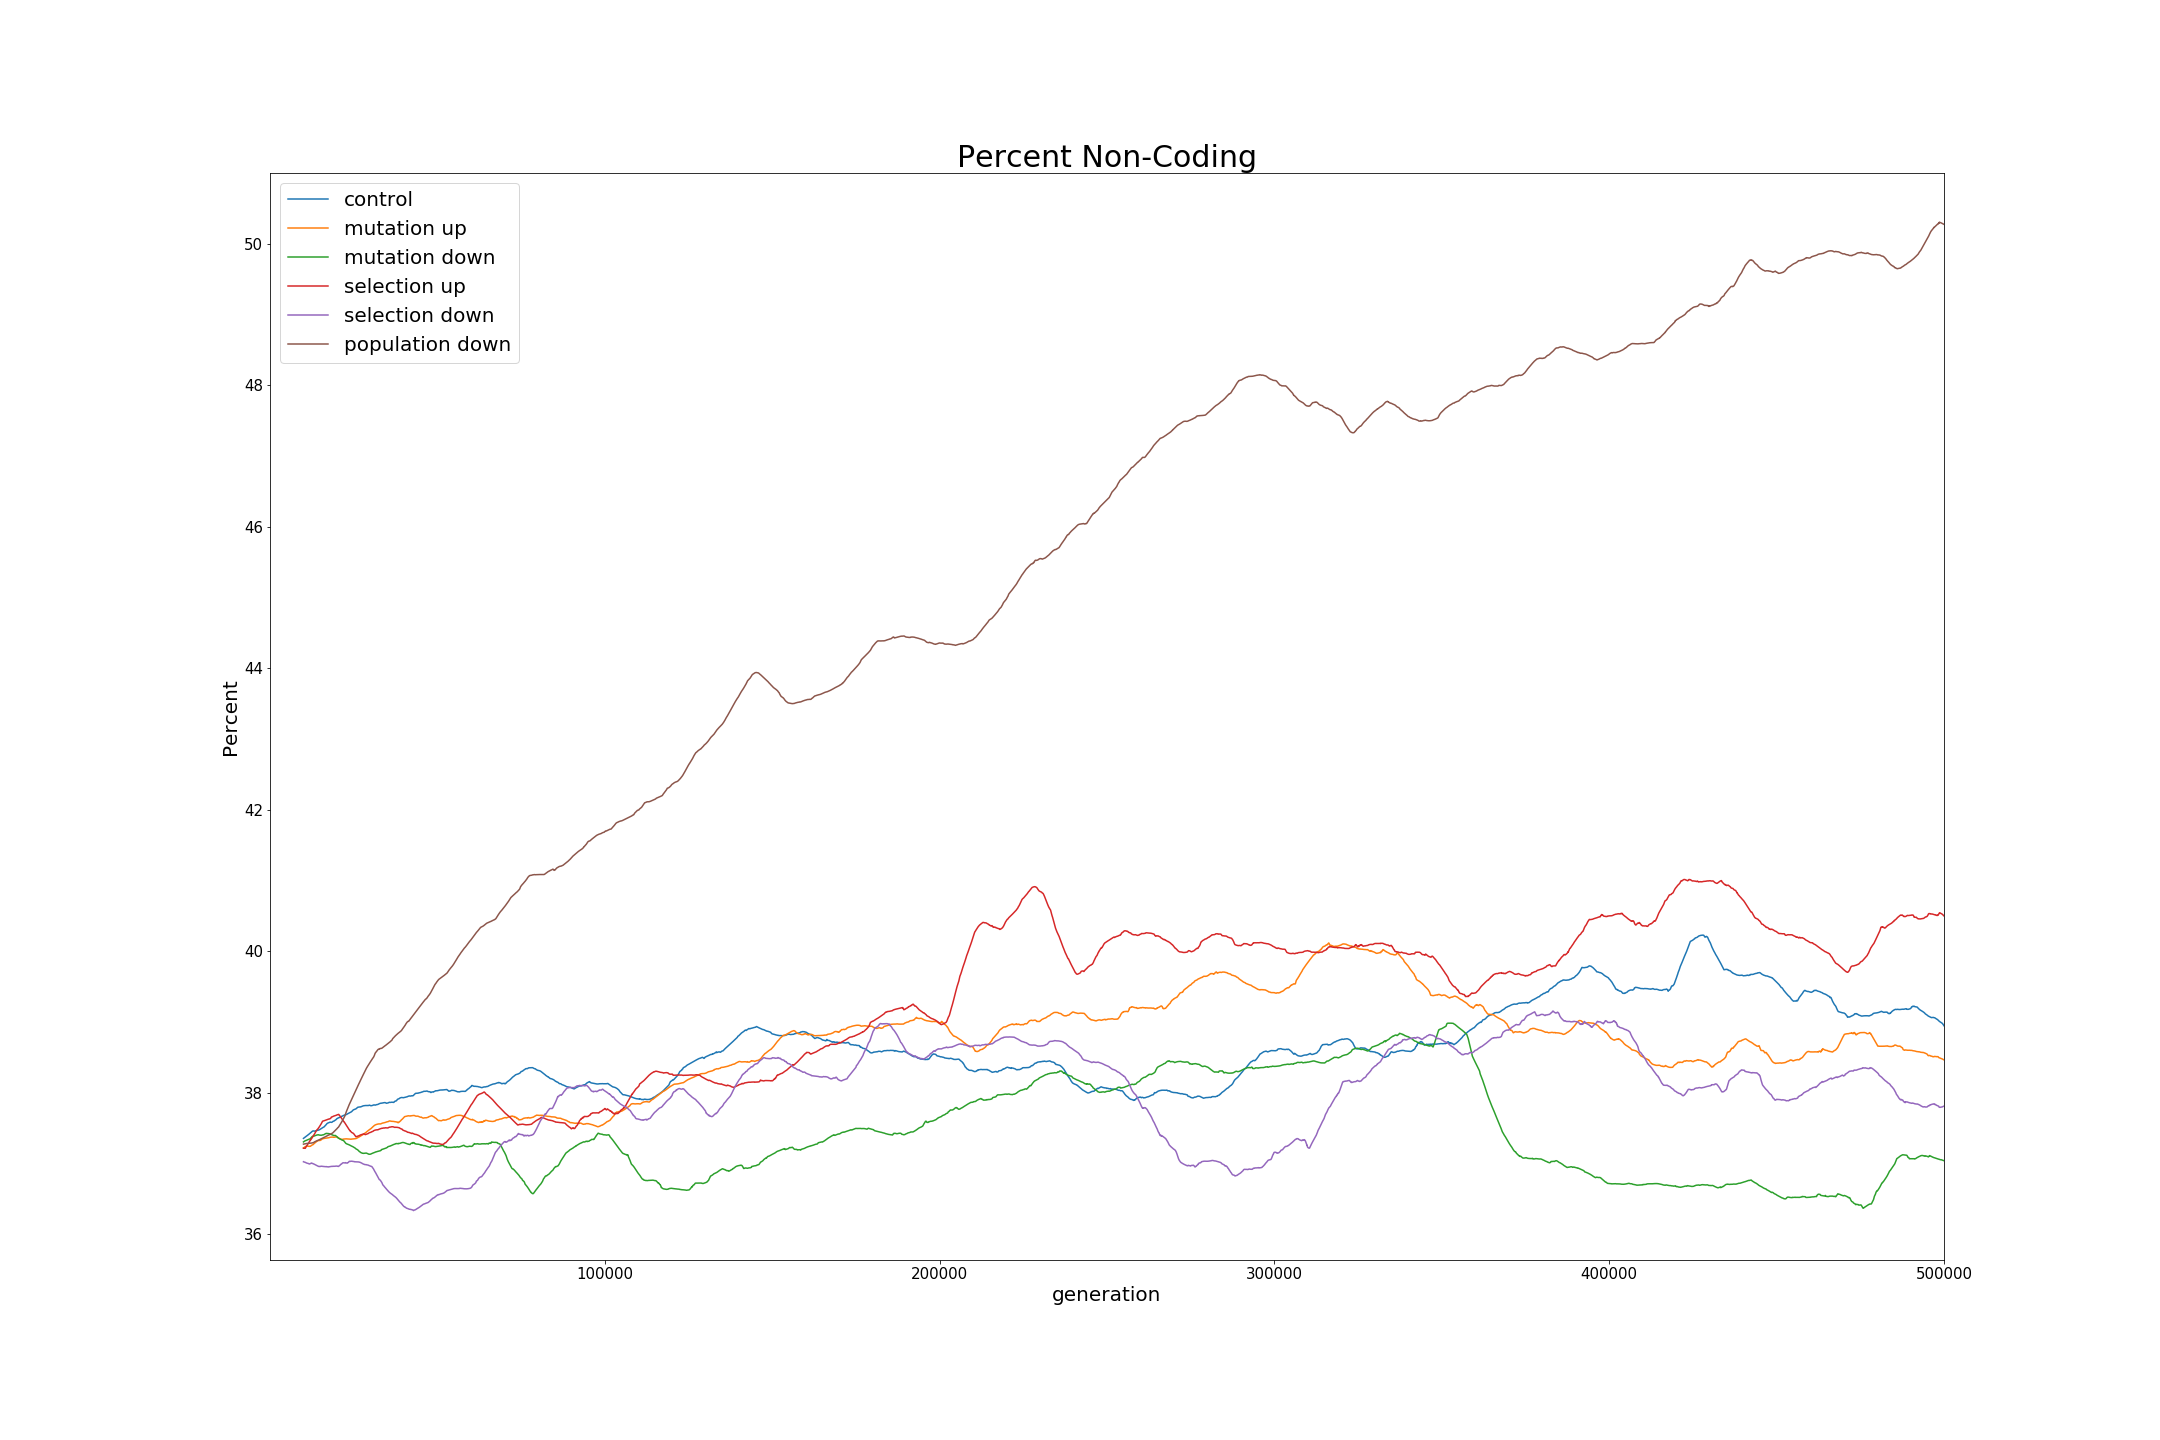
\includegraphics[width=\linewidth]{percent_noncoding}
	\caption[Non-coding DNA]{Plot of the average (across all seeds) number of non-coding bases for the whole population over time for all conditions.}
	\label{fig:mean_non-coding_DNA}
\end{figure}
By comparison, despite the $k_+$ condition's rapid decline in fitness, it did not acquire more than 1\% non-coding DNA. 

The average percentages of non-coding DNA are given in Table~\ref{table:non-coding_DNA_mean_and_standard_deviation} below. 
\begin{table}[H]
	\begin{tabular}{|c|c|c|c|}
		\hline
		\multicolumn{4}{c}{\Large \textbf{\% Non-coding DNA}} \\
		\hline
		& \textbf{mean} & \textbf{standard deviation} & \textbf{mean's \% change from control} \\
		\hline \hline
		control & 38.622711 & 0.601258 & \textemdash \\ 
		\hline
		$\mu_+$ & 38.661764 & 0.707173 & 0.101114 \\ 
		\hline
		$\mu_-$ & 37.446414 & 0.694349 & -3.045608 \\ 
		\hline
		$k_+$ & 39.329164 & 1.138623 & 1.829114 \\ 
		\hline
		$k_-$ & 38.004029 & 0.704953 & -1.601860 \\ 
		\hline
		$N_+$ & 35.881134 & 1.519580 & -7.098353 \\ 
		\hline
		$N_-$ & 45.462209 & 3.545778 & 17.708489 \\ 
		\hline
	\end{tabular}
	\caption[Non-coding DNA mean and standard deviation]{Mean and standard deviation of non-coding percentages of DNA across all seeds.}
	\label{table:non-coding_DNA_mean_and_standard_deviation}
\end{table}

\subparagraph{Number of Functional Genes}\label{sec:number_of_functional_genes}
Recall from Section~\ref{experimental_design} that a ``functional gene'' is a gene which produces a gene product. Specifically in Aevol, this means the production of a triangle of mean $m$, height $h$, and half-width $w$. Figure~\ref{fig:mean_num_functional_genes} below illustrates the mean number of functional genes across the population for each condition.  
\begin{figure}[H]
	\centering
	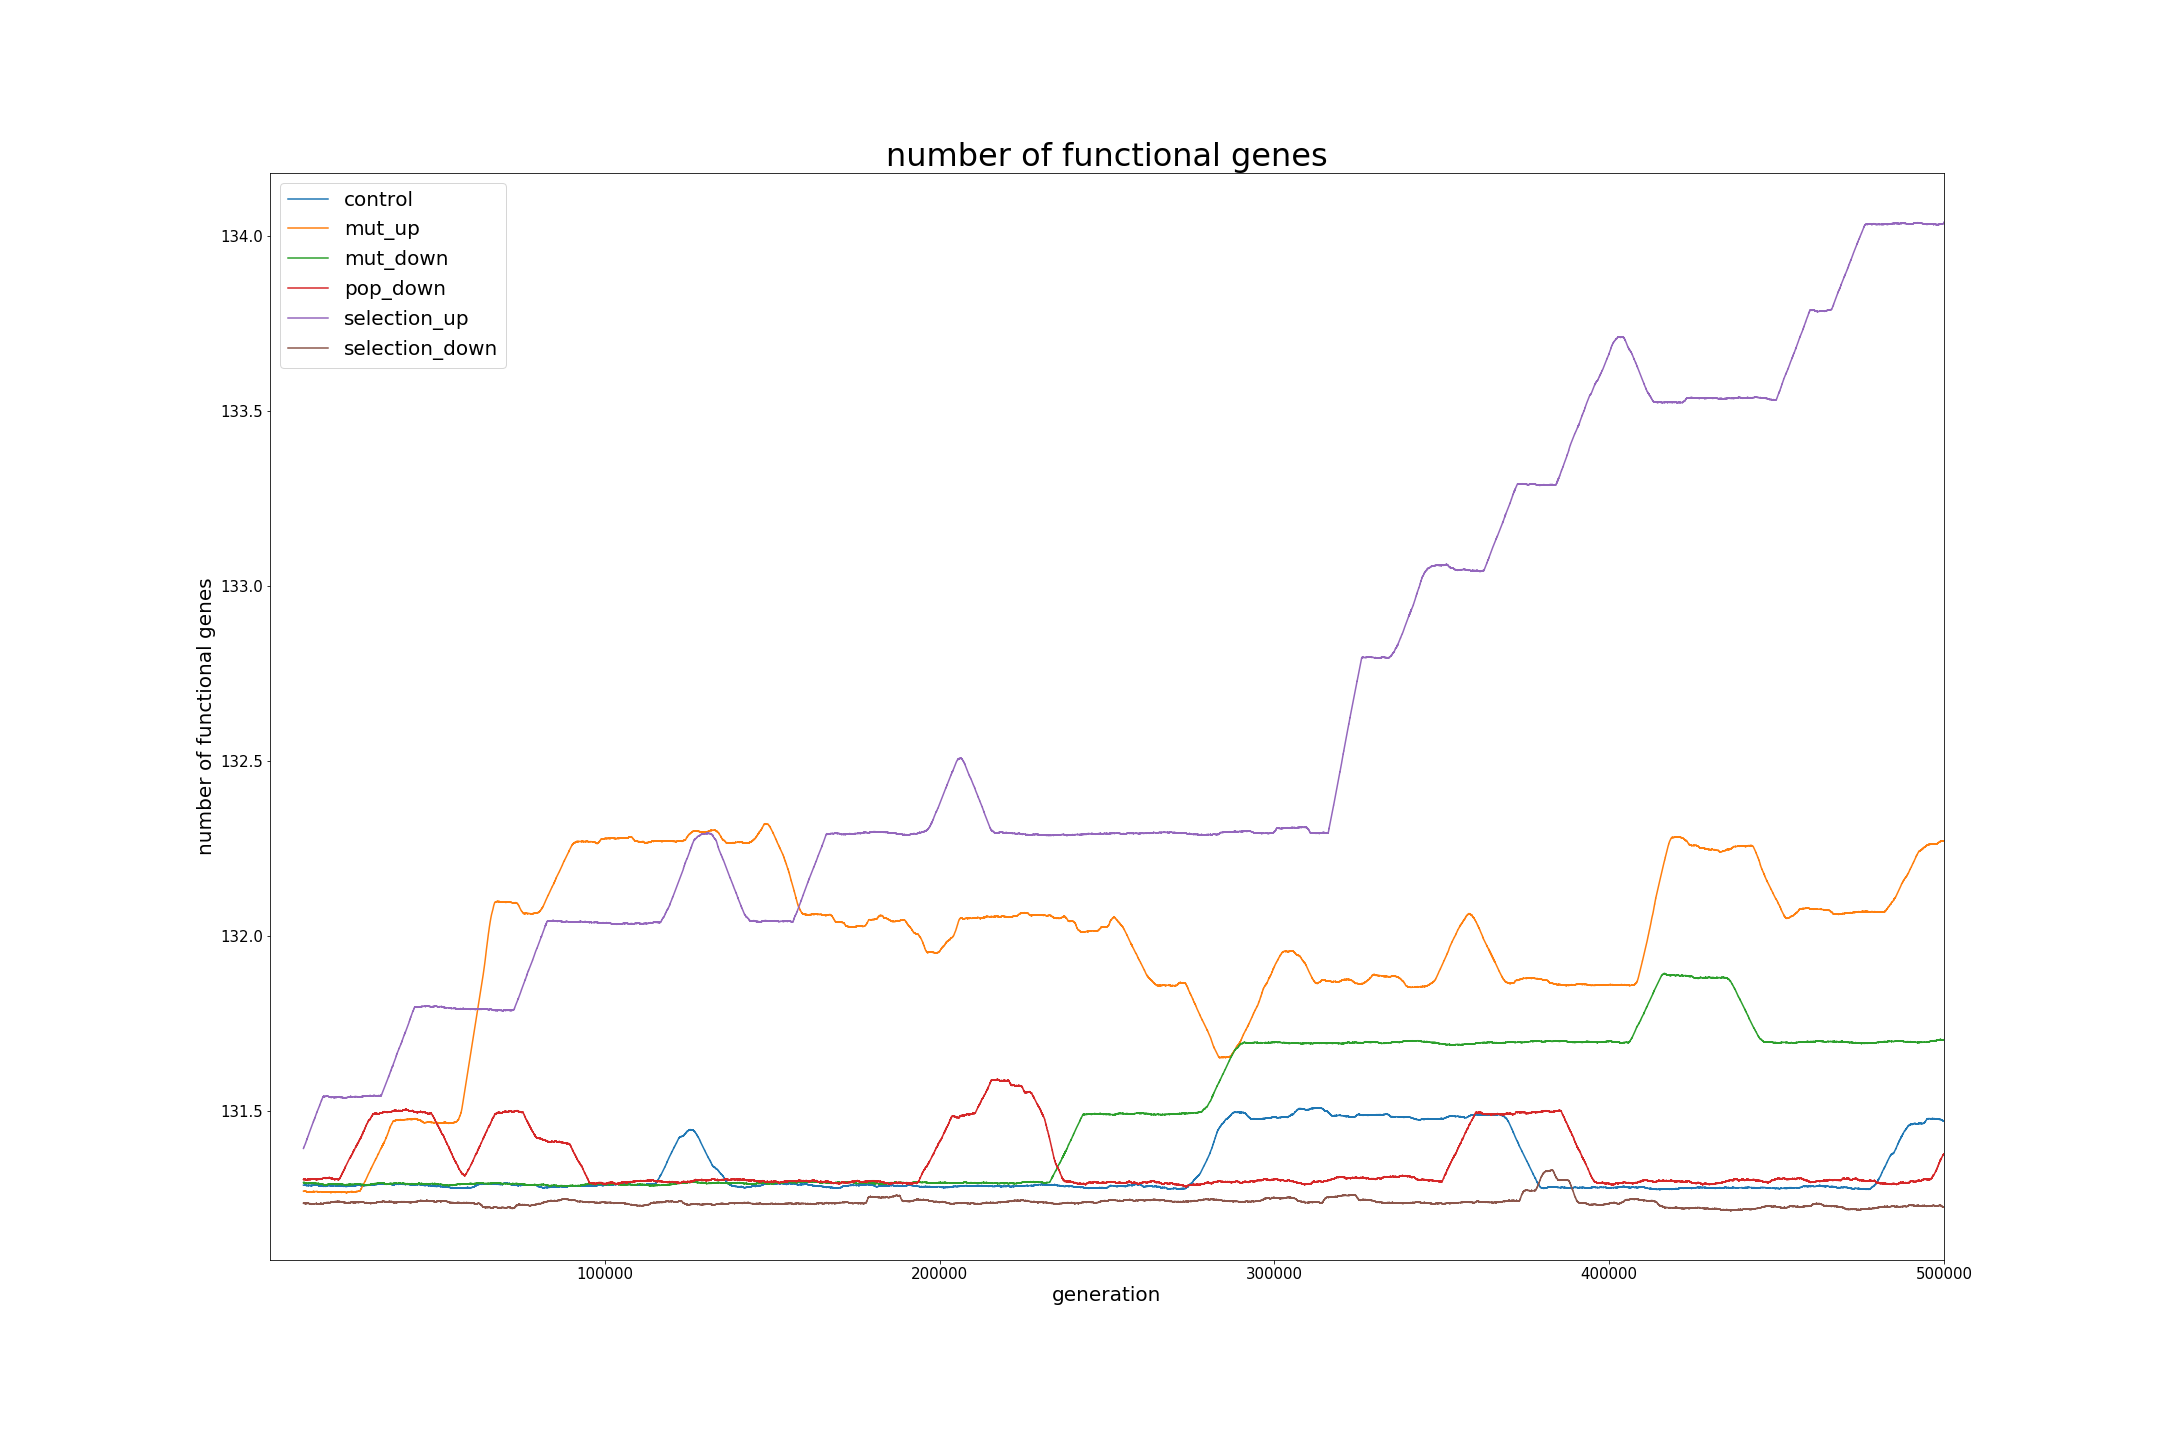
\includegraphics[width=\linewidth]{stat_genes_global_mean_num_functional_genes}
	\caption[Mean number of functional genes]{Plot showing the mean number of functional genes for the population, averaged across all seeds for each condition.}
	\label{fig:mean_num_functional_genes}
\end{figure}
As seen in Figure~\ref{fig:mean_num_functional_genes}, the $k_+$ condition showed the greatest increase in the number of functional genes in the whole population, reaching a maximum increase of about 2.2\% (131 to 134). This is in agreement with the predictions (from Table~\ref{table:experiment_predictions}) and the findings of Knibbe et al.~\cite{Knibbe2007}. Whereas most of the other curves are fairly flat, the mutation up condition fluctuates relatively rapidly, owing to the quick increase and decrease in the number of base pairs. 

The mean and standard deviation of the number of functional genes for the population for each condition is given in Table~\ref{table:number_of_genes_mean_std_dev} below.

\begin{table}[H]
	\centering
	\begin{tabular}{|c|c|c|c|}
		\hline
		\multicolumn{4}{c}{\Large \textbf{Mean Number of Functional Genes}} \\
		\hline
		& \textbf{mean} & \textbf{standard deviation} & \textbf{\% change from control} \\
		\hline
		control & 131.332898 & 0.0815085 & \textemdash \\ 
		\hline
		$\mu_+$ & 131.974778 & 0.252463 & 0.488742 \\ 
		\hline
		$\mu_-$ & 131.500541 & 0.207570 & 0.127647 \\ 
		\hline
		$k_+$ & 132.606568 & 0.719530 & 0.969803 \\ 
		\hline
		$k_-$ & 131.238909 & 0.013974 & -0.071565 \\ 
		\hline
		$N_+$ & 132.378671 & 0.683269 & 0.796276 \\ 
		\hline
		$N_-$ & 131.350519 & 0.083280 & 0.013417 \\ 
		\hline
	\end{tabular}
	\caption[Number of functional genes - mean and standard deviation]{The mean and standard deviation for the number of functional genes of the population, averaged across all seeds and for all conditions.}
	\label{table:number_of_genes_mean_std_dev}
\end{table}
\subparagraph{Number of Non-Functional Genes}\label{results:number_non-functional_genes}
The average number of non-functional genes across all seeds for each condition is illustrated in Figure~\ref{fig:mean_num_non-functional_genes} below, and Table~\ref{table:non-functional_genes_mean_std_dev} provides the mean and standard deviation for all seeds and all conditions.  

\begin{figure}[H]
	\centering
	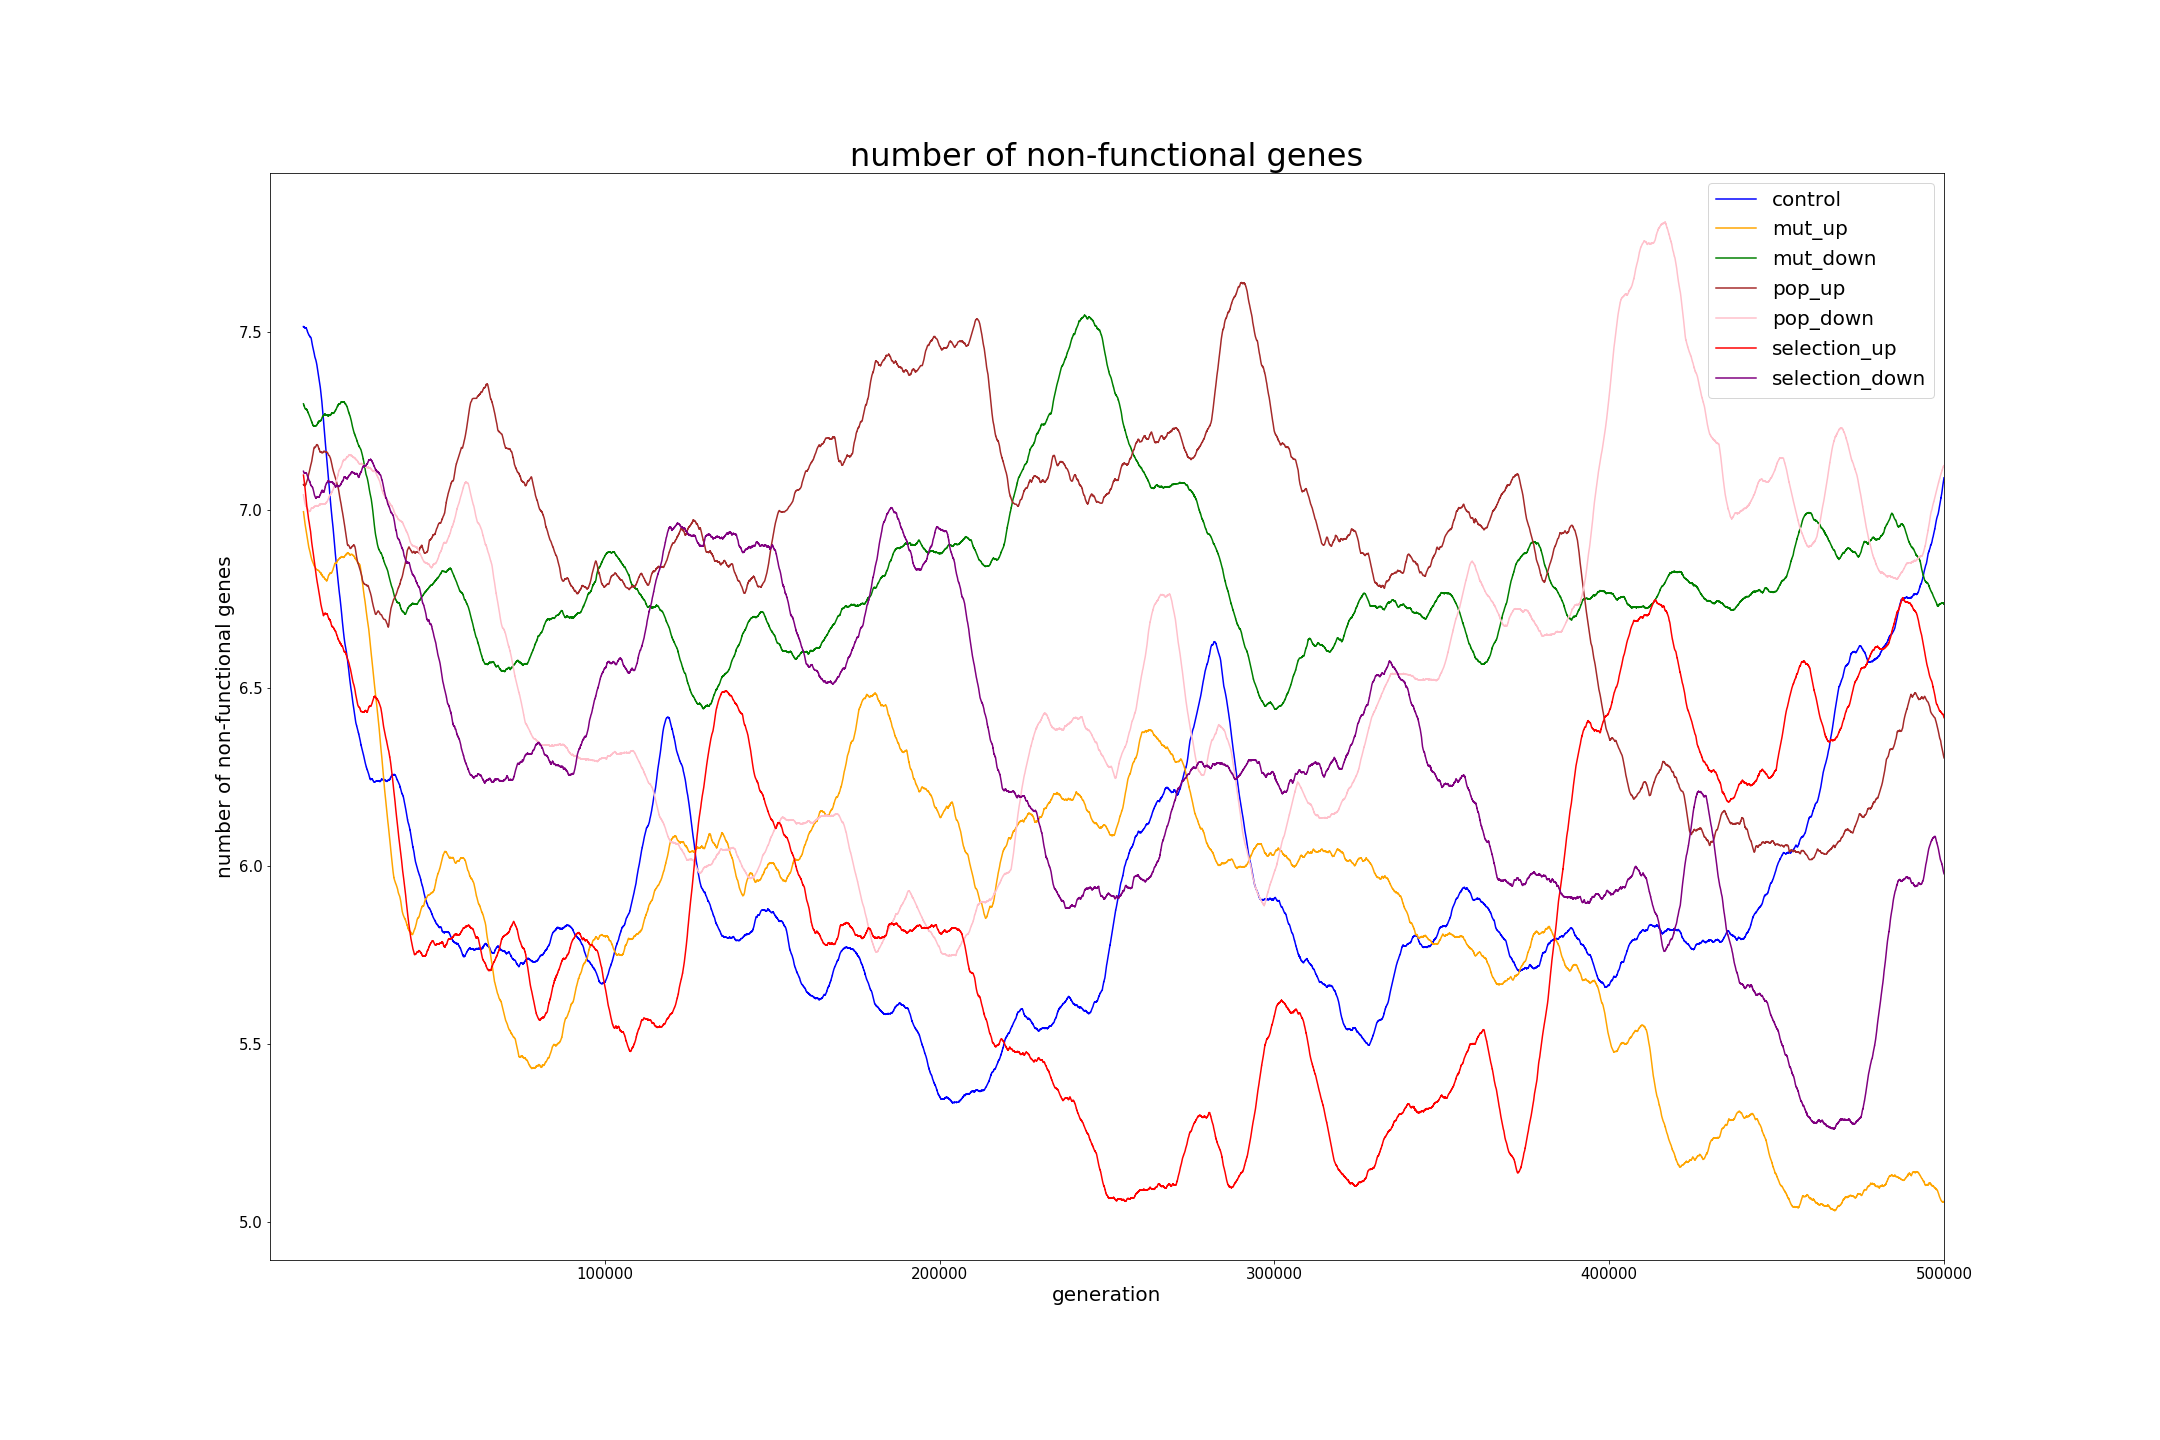
\includegraphics[width=\linewidth]{stat_genes_global_mean_num_non-functional_genes}
	\caption[Mean number of non-functional genes]{The mean number of non-functional genes across all seeds for each condition.}
	\label{fig:mean_num_non-functional_genes}
\end{figure}


\begin{table}[h]
	\centering
	\begin{tabular}{|c|c|c|c|}
		\hline
		\multicolumn{4}{c}{\Large \textbf{Mean Num. Non-Functional Genes (Pseudogenes)}} \\
		\multicolumn{4}{c}{\Large \textbf{Mean \& Std. Dev.}} \\
		\hline
		& \textbf{mean} & \textbf{standard deviation} & \textbf{\% change from control} \\
		\hline
		control & 5.927067 & 0.38579 & \textemdash \\ 
		\hline
		$\mu_+$ & 5.856449 & 0.428473 & -1.191458 \\ 
		\hline
		$\mu_-$ & 6.821348 & 0.221591 & 15.088075 \\ 
		\hline
		$k_+$ & 5.844289 & 0.506922 & -1.396610 \\ 
		\hline
		$k_-$ & 6.297804 & 0.454152 & 6.254978 \\ 
		\hline
		$N_+$ & 6.313992 & 0.329913 & 6.528093 \\ 
		\hline
		$N_-$ & 6.555471 & 0.483631 & 10.602267 \\ 
		\hline
	\end{tabular}
	\caption[Number of Non-functional Genes - Mean \& St. Dev.]{Population mean and standard deviation for the number of non-functional genes, mean of all seeds, all conditions.}
	\label{table:non-functional_genes_mean_std_dev}
\end{table}

\subparagraph{Average Size of Functional Genes}\label{sec:average_size_functional_genes}
Figure~\ref{fig:mean_functional_gene_size} shows the average number of base pairs for each functional gene for the population, mapped out over the 500,000 generations. The population down condition continues to be the outlier in terms of genome structure, with the average size of the functional genes remaining noticeably lower than for any other condition. It is worth pointing out, however, that the difference between the smallest average and the largest average is only 1 base pair. 
\begin{figure}[H]
	\centering
	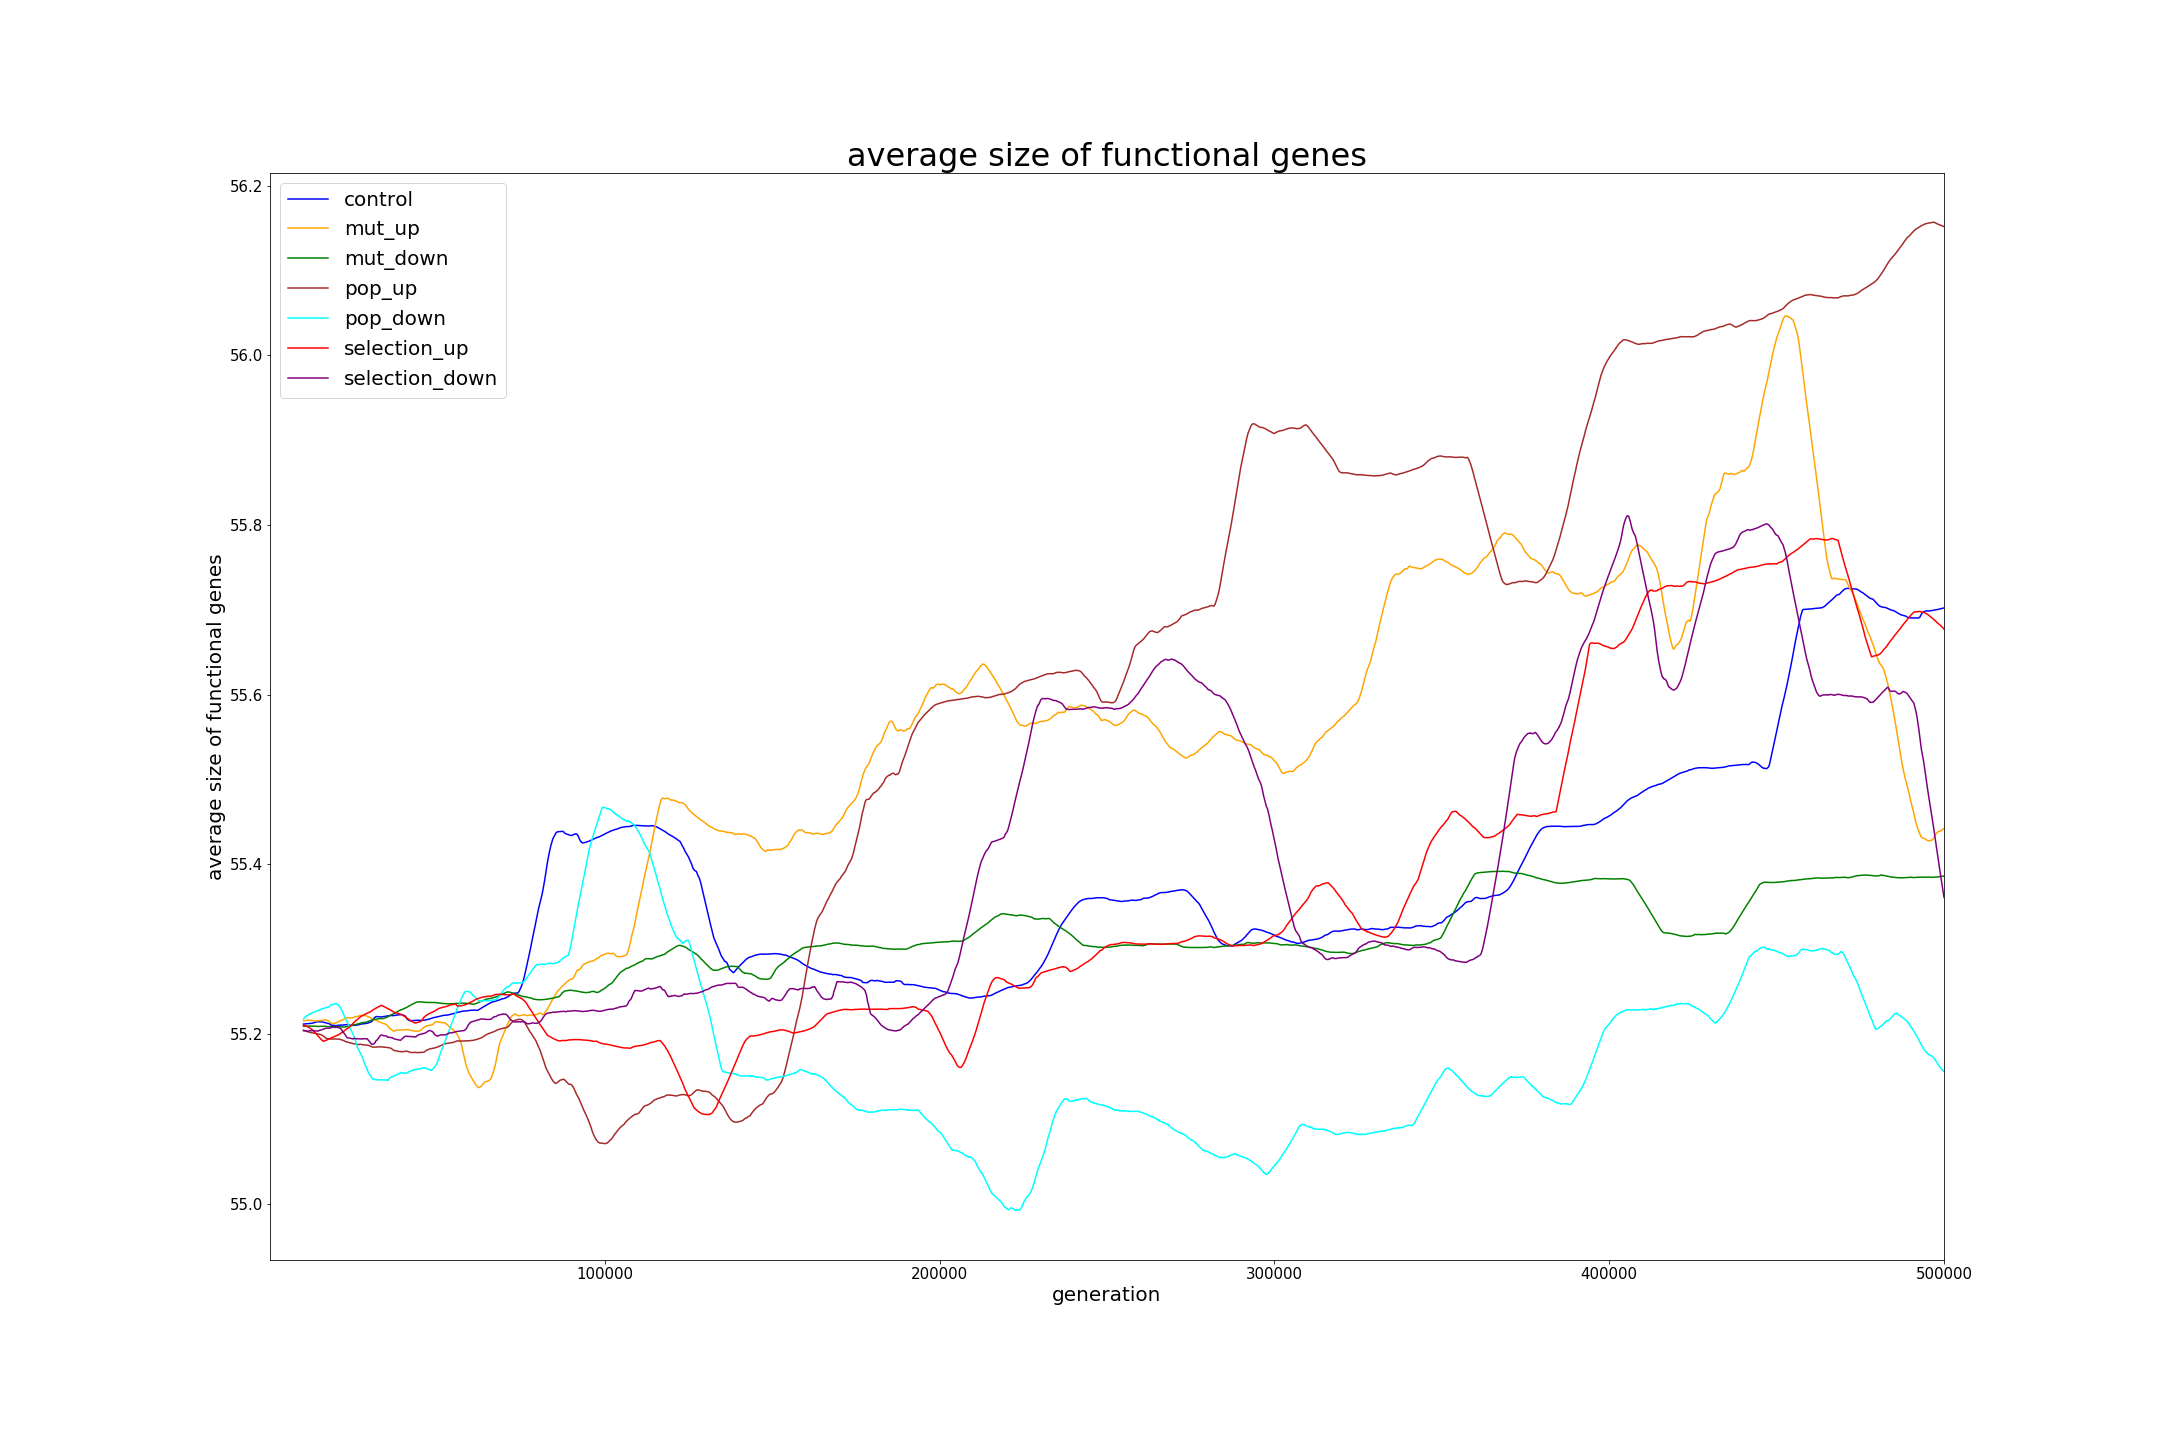
\includegraphics[width=\linewidth]{stat_genes_global_mean_avg_size_of_functional_genes}
	\caption[Average size of functional genes]{Plot showing the average size of functional genes over time for all seeds.}
	\label{fig:mean_functional_gene_size}
\end{figure}
Table~\ref{table:mean_functional_gene_size_and_std_dev} below summarizes the mean and standard deviation of the average size of functional genes for all conditions, and Table~\ref{table:avg_size_of_functional_genes_rank_sum_and_p-value} gives the p-values for comparing the control condition to every other condition. 

\begin{table}[H]
	\centering
	\begin{tabular}{|c|c|c|c|}
		\hline
		\multicolumn{4}{c}{\Large \textbf{Average size of functional genes}} \\
		\hline
		& \textbf{mean} & \textbf{standard deviation} & \textbf{\% change from control} \\
		\hline
		control & 55.375430 & 0.137457 & \textemdash \\ 
		\hline
		$\mu_+$ & 55.542625 & 0.207164 & 0.301929 \\ 
		\hline
		$\mu_-$ & 55.309915 & 0.050594 & -0.118309 \\ 
		\hline
		$k_+$ & 55.370465 & 0.202443 & -0.008965 \\ 
		\hline
		$k_-$ & 55.414465 & 0.195425 & 0.070492 \\ 
		\hline
		$N_+$ & 55.460664 & 0.225992 & 0.153921 \\ 
		\hline
		$N_-$ & 55.174290 & 0.098860 & -0.363230 \\ 
		\hline
	\end{tabular}
	\caption[Mean functional gene size and standard deviation]{Mean functional gene size and standard deviation, all seeds, all conditions.}
	\label{table:mean_functional_gene_size_and_std_dev}
\end{table}

\begin{table}[H]
	\begin{tabular}{|c|c|c|}
		\hline
		\multicolumn{3}{c}{\Large \textbf{Average size of functional genes - rank sum \& p-value}} \\
		\hline
		& \textbf{rank sum} & \textbf{p-value} \\
		\hline
		control & 124950901896.50 & 0.36686747 \\ 
		\hline
		$\mu_+$ & 68252491056.00 & 0.00000000 \\ 
		\hline
		$\mu_-$ & 96067062201.50 & 0.00000000 \\ 
		\hline
		$N_+$ & 102626876736.00 & 0.00000000 \\ 
		\hline
		$N_-$ & 28963878467.00 & 0.00000000 \\ 
		\hline
		$k_+$ & 103481641646.00 & 0.00000000 \\ 
		\hline
		$k_-$ & 124890321462.00 & 0.22366471 \\ 
		\hline
	\end{tabular}
	\caption[Average size of functional genes - rank sum and p-value]{Average size of functional genes - rank sum and p-value for all conditions and all seeds.}
	\label{table:avg_size_of_functional_genes_rank_sum_and_p-value}
\end{table}
Since the $k_-$ condition's p-value was $\geq0.05$, it must be concluded that these results are not significant. 

\subsection{Evolvability}\label{res:evolvability}
In Figure~\ref{fig:evolvability_all_seeds} below, the results of the experiments on evolvability for the best individual's (at generation 500,000) lineage are shown. 
\begin{figure}[H]
	\centering
	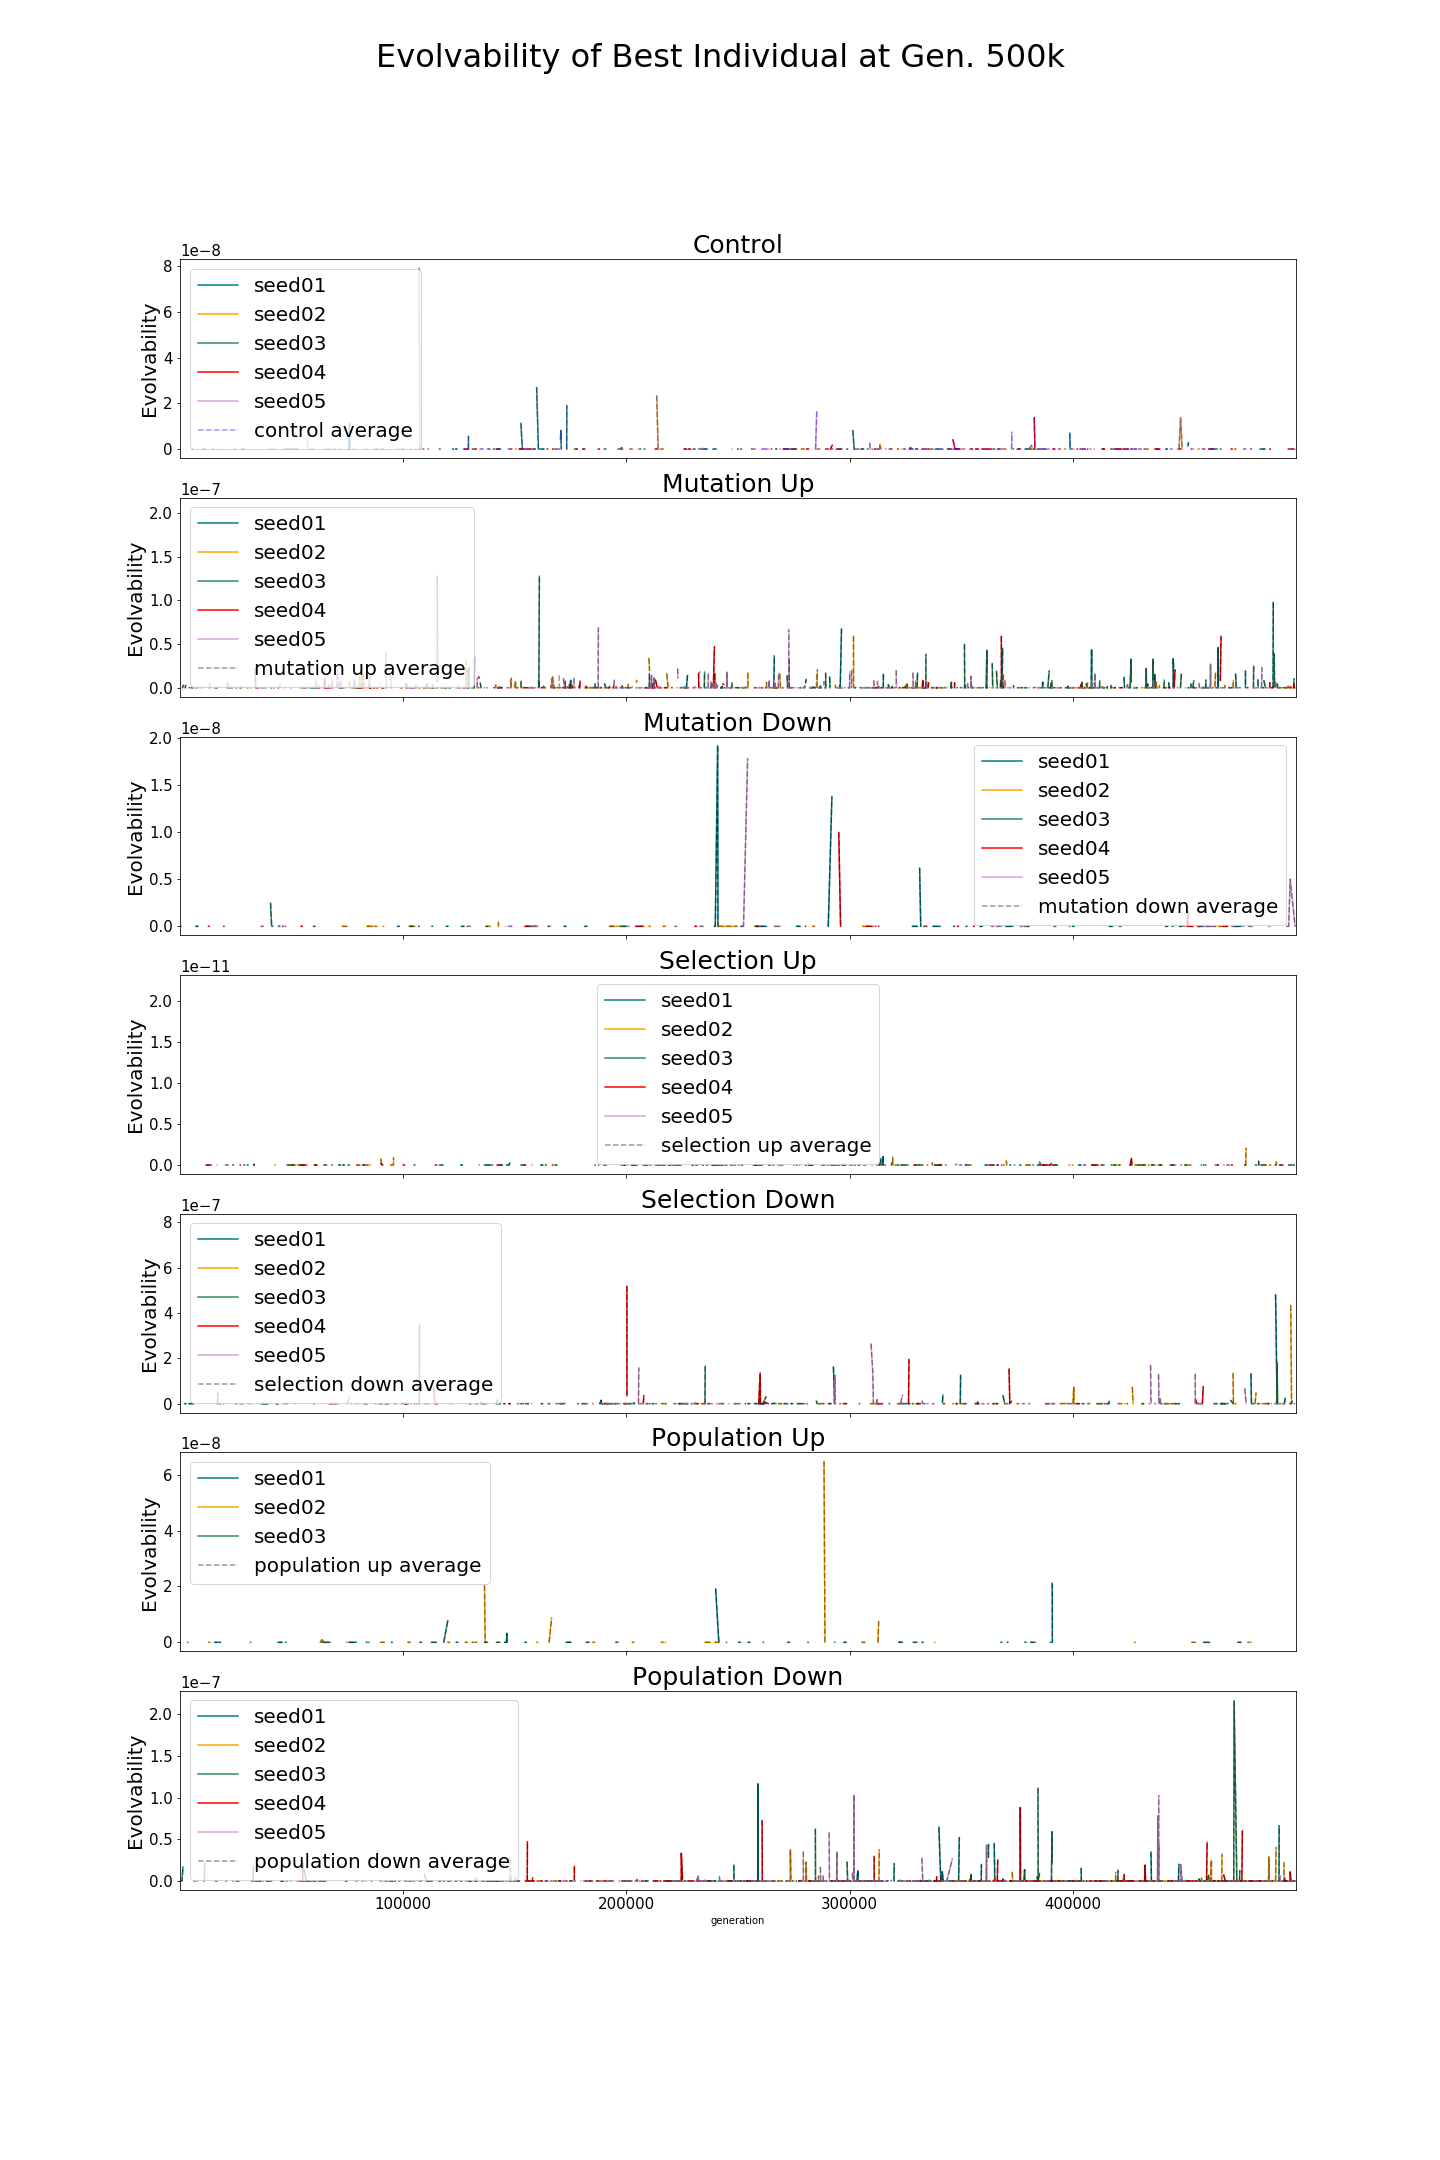
\includegraphics[width=\linewidth]{evolvability_plot_all_seeds01}
	\caption[Evolvability plot, all seed]{A plot showing the evolvability of all seeds and all conditions. Larger numbers are more evolvable (mind the scale for each condition, upper left).}
	\label{fig:evolvability_all_seeds}	
\end{figure}

The evolvability rank sum and p-value information is given in Table~\ref{table:evolvability-rank_sum_and_p-values}.

\begin{table}[H]
	\begin{tabular}{|c|c|c|}
		\hline
		\multicolumn{3}{c}{\Large \textbf{Evolvability rank sum and p-value}} \\
		\hline
		& \textbf{rank sum} & \textbf{p-value} \\
		\hline
		$\mu_+$ & 37476904.00 & 0.11538726 \\ 
		\hline
		$\mu_-$ & 4084573.50 & 0.00000000 \\ 
		\hline
		$N_+$ & 101772759.00 & 0.00000000 \\ 
		\hline
		$N_-$ & 15367560.00 & 0.00000000 \\ 
		\hline
		$k_+$ & 6997351.00 & 0.00000000 \\ 
		\hline
		$k_-$ & 8535654.00 & 0.00000000 \\ 
		\hline
	\end{tabular}
	\caption[Evolvability - rank sum and p-value]{Rank sum and p-values for evolvability, all seeds, all conditions.}
	\label{table:evolvability-rank_sum_and_p-values}
\end{table}

\begin{table}[H]
	\centering
	\begin{tabular}{| c | c | c | c |}
		\hline
		\multicolumn{4}{c}{\Large Evolvability - Mean \& Std. Dev.} \\
		\hline
		& \textbf{mean} & \textbf{standard deviation} & \textbf{\% change from control} \\
		\hline
		\hline
		control & 4.133535e-10 & 3.28521e-09 & \textemdash \\ 
		\hline
		$\mu_+$ & 1.789394e-09 & 7.828305e-09 & 332.8969 \\ 
		\hline
		$\mu_-$ & 1.369594e-10 & 1.320591e-09 & -66.86627 \\ 
		\hline
		$k_+$ & 4.152320e-14 & 6.590472e-13 & -99.98995 \\ 
		\hline
		$k_-$ & 8.394271e-09 & 5.085889e-08 & 1930.773 \\ 
		\hline
		$N_+$ & 8.149206e-10 & 4.345602e-09 & 97.14859 \\ 
		\hline
		$N_-$ & 1.015906e-09 & 8.152163e-09 & 145.7718 \\ 
		\hline	 		 
	\end{tabular}
	\caption[Evolvability mean and standard deviation]{Table illustrating the mean and standard deviation of the evolvability for each condition. $\mu$ is the mutation rate, $k$ is the selection rate, and $N$ is the population size.}
	\label{table:mean_std_dev_evolvability}
\end{table}

\subsection{Robustness}
Recall from Section~\ref{subsec:robustness_antirobustness} that robustness is measured by the fraction of neutral offspring of an individual. In the following figure, a bar plot showing the spread of neutral offspring for the best individual is seen for the control condition as well as the six variations. 

\begin{figure}[H]
	\centering
	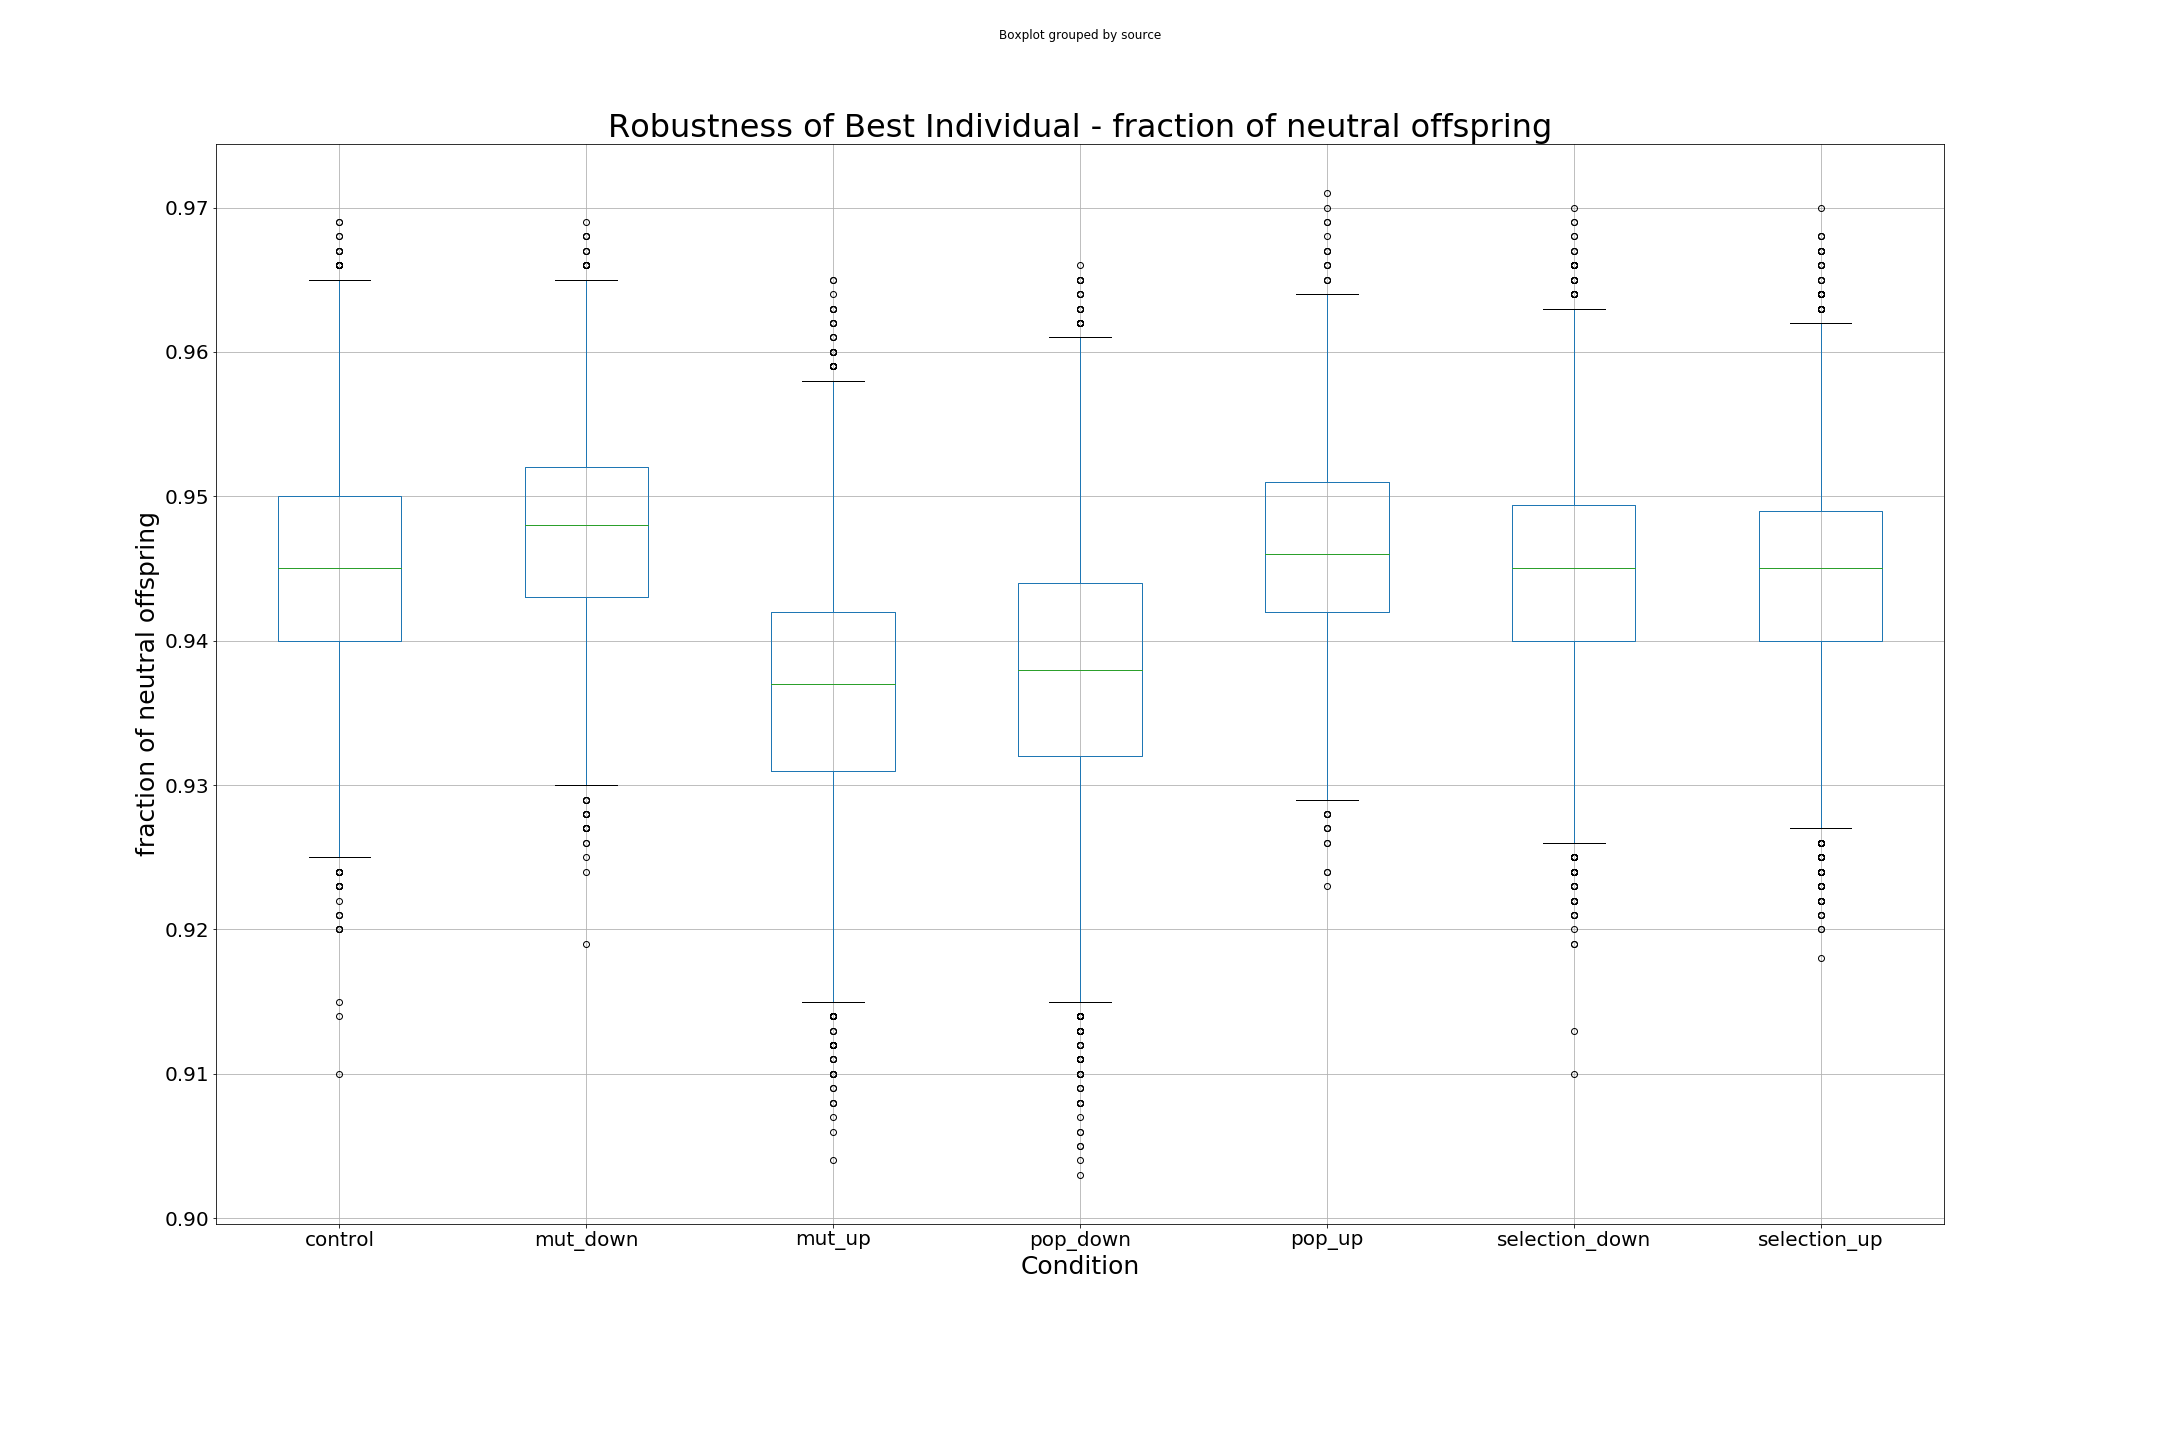
\includegraphics[width=\linewidth]{stat_robustness_best_mean_frac_neutral_offspring}
	\caption[Robustness box and whisker plot]{A box and whisker plot showing the spread of neutral offspring for the best individual at generation 500,000, all conditions. Higher numbers are more robust.}
	\label{fig:mean_robustness_all_conditions}
\end{figure}
The mutation up condition clearly had the largest mean percentage of neutral mutants, at 0.5\%. The full statistics are given in the tables below. Since the $k_-$ condition's p-value was $\geq0.5$, it must be rejected.

\begin{table}
	\begin{tabular}{|c|c|c|}
		\hline
		\multicolumn{3}{c}{\Large \textbf{Robustness - Rank Sum \& p-values}} \\
		\hline
		& \textbf{rank sum} & \textbf{p-value} \\
		\hline
		$\mu_+$ & 6888635.50 & 0.00000000 \\ 
		\hline
		$\mu_-$ & 3858925.50 & 0.00000000 \\ 
		\hline
		$k_+$ & 13792971.00 & 0.04364015 \\ 
		\hline
		$k_-$ & 14320878.00 & 0.28251799 \\ 
		\hline
		$N_+$ & 9467109.50 & 0.00000000 \\ 
		\hline
		$N_-$ & 15908963.00 & 0.00000000 \\ 
		\hline
	\end{tabular}
	\caption[Robustness rank sum \& p-values]{Mean robustness rank sum and p-values for all conditions and all seeds.}
	\label{table:robustness_rank_sum_p-values}
\end{table}

\begin{table}[H]
	\begin{tabular}{|c|c|c|c|}
		\hline
		\multicolumn{4}{c}{\Large \textbf{Robustness - means \& standard deviations}} \\
		\hline
		& \textbf{mean} & \textbf{std. dev.} & \textbf{mean's \% change from control} \\
		\hline
		control & 0.001470 & 0.00121821 & \textemdash \\ 
		\hline
		$\mu_+$ & 0.004852 & 0.002302 & 230.026777 \\ 
		\hline
		$\mu_-$ & 0.000545 & 0.000753 & -62.935291 \\ 
		\hline
		$k_+$ & 0.001427 & 0.001196 & -2.906602 \\ 
		\hline
		$k_-$ & 0.001481 & 0.001215 & 0.725871 \\ 
		\hline
		$N_+$ & 0.001181 & 0.001106 & -19.645748 \\ 
		\hline
		$N_-$ & 0.002449 & 0.001702 & 66.563607 \\ 
		\hline
	\end{tabular}
	\caption[Robustness means and standard deviations]{Robustness means and standard deviations for all conditions and all seeds.}
	\label{table:robustness_means_and_std_dev}
\end{table}

\section{Discussion}\label{discussion}

Analogously to Table~\ref{table:experiment_predictions}, the results of the experiments in Table~\ref{table:experiment_results_summary} are summarized below. For each cell, {\color{green} green} indicates that the prediction was confirmed in these experiments and {\color{red}red} indicates that the prediction must be rejected. The predictions for each condition are duplicated here for convenience, with a $+$ indicating a predicted increase and $-$ indicating a predicted decrease over the control condition. 

\begin{table}[H]
	\centering
	\begin{tabular}{|c||c|c|c|c|c|c|}
		\hline
		\multicolumn{7}{|c|}{{\Large \textbf{Experiment Results Summary}}} \\
		\hline \hline
		\multirow{2}{*}{\textbf{Effect On:}} & \multicolumn{6}{c|}{\textbf{Condition}} \\
		\cline{2-7}
		& {\Large$\mu_+$} & {\Large$\mu_-$} & {\Large$k_+$} & {\Large$k_-$} & {\Large$N_+$} & {\Large$N_-$} \\
		\hline 
		Genome Size & \cellcolor{green} - & \cellcolor{red} + & \cellcolor{green} + & \cellcolor{green} - & \cellcolor{green} - & \cellcolor{green} + \\
		\hline
		Fitness & \cellcolor{green} + & \cellcolor{green} - & \cellcolor{red} + & \cellcolor{red} - & \cellcolor{green} + & \cellcolor{green} - \\
		\hline
		Amount of non-coding DNA & \cellcolor{green} - & \cellcolor{red} + & \cellcolor{green} + & \cellcolor{green} - & \cellcolor{green} - & \cellcolor{green} + \\
		\hline
		Number of genes & \cellcolor{red} - & \cellcolor{green} + &\cellcolor{green} + & \cellcolor{green} - & \cellcolor{red} - & \cellcolor{green} + \\
		\hline
		Average size of genes & \cellcolor{red} - & \cellcolor{green} + & \cellcolor{green} - & \cellcolor{red} + & \cellcolor{green} - & \cellcolor{red} + \\
		\hline
		Robustness & \cellcolor{green} - &\cellcolor{green} + & \cellcolor{green} - & \cellcolor{green}+ & \cellcolor{green} - & \cellcolor{red} + \\
		\hline
		Evolvability &\cellcolor{green} + &\cellcolor{green} - & \cellcolor{red}  + & \cellcolor{red} - & \cellcolor{red} - & \cellcolor{green} + \\
		\hline		
	\end{tabular}
	\caption[Experiment result summary]{A summary of whether the experiment results confirmed or denied the hypotheses of Table~\ref{table:experiment_predictions}.  were confirmed ({\color{green}green}) or rejected ({\color{red}red}), along with the predicted results of whether the given result would increase (+) or decrease (-) over the control condition.}
	\label{table:experiment_results_summary}
\end{table}

The largest driver of reductive evolution in these experiments, as summarized by Table~\ref{table:genome_size_mean_and_std_dev}, was clearly increasing the population size. The efficacy of selection to overcome genetic drift was greatly increased by the availability of greater genetic variance in the larger population. 

\subsection{Genome Size}

According to the predictions based on a survey of the literature (as summarized in Table~\ref{table:experiment_predictions}), only the $\mu_+$, $k_-$, and $N_+$ conditions were predicted to lead to a reduced genome. As shown in Figure~\ref{fig:genome_size}, however, although the $\mu_+$ and $k_-$ conditions did end up with a genome size which was noticeably smaller than the control condition, surprisingly $\mu_-$ also experienced a reduction in genome size. 



\subsection{Metabolic Error and Fitness}
Examining Figure~\ref{fig:mean_fitness_all_seeds}, it quickly becomes apparent that, in the static environment in which the wild type evolved, adding another 500,000 generations on top of the previous 10 million does not much affect the average fitness of the control condition. Small fluctuations occurred due to mutations, insertions, etc. but overall the genotype was quite steady. However, for the $\mu_+$, $\mu_-$, $k_+$, and $N_+$ conditions, a clear trend towards improved fitness may be observed.

More interesting are the $N_-$ and $k_+$ conditions, where by generation 500,000 the average fitness in the whole population declined to 2.76\% and 99.99\% below the control condition respectively (see Table~\ref{table:fitness_means_std_dev}). It seems that with the smaller population size, genetic drift may be more strongly at work in continually increasing the gap between the phenotype and environmental function, as the lack of variety inherent in a smaller population causes a cascade of increasingly deleterious consequences.
 
\subsection{Functional Genes}
Regarding the $N_-$ condition, comparing this with the results of Batut et al. and their work with \textit{Buchnera aphidicola} (see Section~\ref{related_work}), it may be possible that gene loss is occurring because of the smaller effective population size clicking down Muller's ratchet. This does not seem to be what is happening in these experiments either, however. Though mean fitness of the $N_-$ condition did greatly decline (see Figure~\ref{fig:mean_fitness_plot}), the $N_-$ condition also saw the largest accumulation of non-coding DNA (see Figure~\ref{fig:mean_non-coding_DNA}) and the second-highest level of evolvability (see Table~\ref{table:mean_std_dev_evolvability}), which should theoretically have lead to an easier time of overcoming the ratchet. On the other hand, the number of functional genes stayed more or less the same as all of the other conditions, and the accumulated number of non-functional genes (pseudogenes) of the $N_-$ condition was the largest (see Figure~\ref{fig:mean_num_non-functional_genes}). These two factors together suggest that there almost certainly was some loss of fitness through pseudogenization; perhaps with more time, the pseudogenes would also have been lost.

Recall the work of Liard et al.\cite{Liard.2018} as discussed in Section~\ref{related_work}, in which the proposed ``complexity ratchet'' was overcome by increasing the mutation rate. Their work was quite successful in overcoming this ratchet, but in the experiments of this thesis, both the number of genes and the average size of the genes increased. One possible explanation for this is that, in their work, their increased mutation rate $\mu_+$ was set to $1e^{-3}$.  By contrast, even the elevated mutation rate used here, $\mu_+$, was just $4e^{-7}$, which is $\frac{1}{4}*e^4 \approx 13.65$ times lower than their highest mutation rate. Perhaps an even higher mutation rate would be sufficient to overcome the power of selection and reduce the genome further. 

\section{Results Summary}
Connecting it all together, there is, then, a natural link between the amount of non-coding DNA, coding DNA, genome size, evolvability, robustness, and selection. As the amount of non-coding bases (and therefore overall genome size) increases through natural mutational processes, these non-coding bases can nevertheless play a crucial role in increasing evolvability by being the fodder for new potentially beneficial mutations~\cite{Knibbe2007}. However, a trade-off exists because the increased \textit{mutational load} (i.e. the increasing cost of recurrent harmful mutations, as most mutations are) also carries a fitness cost. In a population whose effective population size is too small, these deleterious mutations accumulate, a phenomenon known as Muller's ratchet~\cite{MullersRatchet}. 

Liard et al.~\cite{Liard.2018} demonstrated, however, that this ``complexity ratchet'' (i.e. the tendency of genomes to become larger and more complex) is not impossible to overcome, and selecting for robustness is an effective strategy for overcoming the ratchet. 




